% Options for packages loaded elsewhere
\PassOptionsToPackage{unicode}{hyperref}
\PassOptionsToPackage{hyphens}{url}
%
\documentclass[
]{book}
\usepackage{lmodern}
\usepackage{amssymb,amsmath}
\usepackage{ifxetex,ifluatex}
\ifnum 0\ifxetex 1\fi\ifluatex 1\fi=0 % if pdftex
  \usepackage[T1]{fontenc}
  \usepackage[utf8]{inputenc}
  \usepackage{textcomp} % provide euro and other symbols
\else % if luatex or xetex
  \usepackage{unicode-math}
  \defaultfontfeatures{Scale=MatchLowercase}
  \defaultfontfeatures[\rmfamily]{Ligatures=TeX,Scale=1}
\fi
% Use upquote if available, for straight quotes in verbatim environments
\IfFileExists{upquote.sty}{\usepackage{upquote}}{}
\IfFileExists{microtype.sty}{% use microtype if available
  \usepackage[]{microtype}
  \UseMicrotypeSet[protrusion]{basicmath} % disable protrusion for tt fonts
}{}
\makeatletter
\@ifundefined{KOMAClassName}{% if non-KOMA class
  \IfFileExists{parskip.sty}{%
    \usepackage{parskip}
  }{% else
    \setlength{\parindent}{0pt}
    \setlength{\parskip}{6pt plus 2pt minus 1pt}}
}{% if KOMA class
  \KOMAoptions{parskip=half}}
\makeatother
\usepackage{xcolor}
\IfFileExists{xurl.sty}{\usepackage{xurl}}{} % add URL line breaks if available
\IfFileExists{bookmark.sty}{\usepackage{bookmark}}{\usepackage{hyperref}}
\hypersetup{
  pdftitle={UC UAS Policy Guidance Document},
  pdfauthor={Dr.~Brandon Stark},
  hidelinks,
  pdfcreator={LaTeX via pandoc}}
\urlstyle{same} % disable monospaced font for URLs
\usepackage{longtable,booktabs}
% Correct order of tables after \paragraph or \subparagraph
\usepackage{etoolbox}
\makeatletter
\patchcmd\longtable{\par}{\if@noskipsec\mbox{}\fi\par}{}{}
\makeatother
% Allow footnotes in longtable head/foot
\IfFileExists{footnotehyper.sty}{\usepackage{footnotehyper}}{\usepackage{footnote}}
\makesavenoteenv{longtable}
\usepackage{graphicx,grffile}
\makeatletter
\def\maxwidth{\ifdim\Gin@nat@width>\linewidth\linewidth\else\Gin@nat@width\fi}
\def\maxheight{\ifdim\Gin@nat@height>\textheight\textheight\else\Gin@nat@height\fi}
\makeatother
% Scale images if necessary, so that they will not overflow the page
% margins by default, and it is still possible to overwrite the defaults
% using explicit options in \includegraphics[width, height, ...]{}
\setkeys{Gin}{width=\maxwidth,height=\maxheight,keepaspectratio}
% Set default figure placement to htbp
\makeatletter
\def\fps@figure{htbp}
\makeatother
\setlength{\emergencystretch}{3em} % prevent overfull lines
\providecommand{\tightlist}{%
  \setlength{\itemsep}{0pt}\setlength{\parskip}{0pt}}
\setcounter{secnumdepth}{5}
\usepackage{booktabs}
\usepackage[margin=1.0in]{geometry}
\usepackage{parskip}
\usepackage{titletoc}
\usepackage[hyphens]{url}
\usepackage{pifont}
\usepackage{amsmath}
\usepackage{amsfonts}
\usepackage{amssymb}



\usepackage{tcolorbox}



\newtcolorbox{content-box}[2][]{
     colback=#2!10,
     colframe=#2!20,
     boxsep=5pt,
     #1,
}
\newenvironment{titlet}{\bfseries}{\hline}
\usepackage[]{natbib}
\bibliographystyle{apalike}

\title{UC UAS Policy Guidance Document}
\author{Dr.~Brandon Stark}
\date{2020-06-05}

\begin{document}
\maketitle

{
\setcounter{tocdepth}{1}
\tableofcontents
}
\hypertarget{preface}{%
\chapter*{Preface}\label{preface}}
\addcontentsline{toc}{chapter}{Preface}

\begin{center}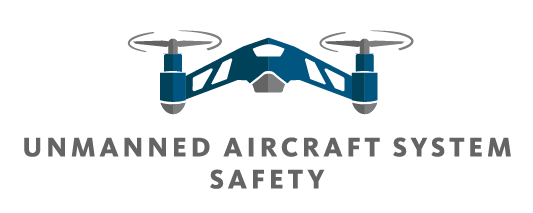
\includegraphics[width=0.5\linewidth]{images/COE_logo} \end{center}

The \textbf{UC Center of Excellence on Unmanned Aircraft System Safety} provides the following non-binding guidance to assist in the implementation of the Presidential Unmanned Aircraft System Policy (Policy), including the management of UAS Activity at University ocations and the development of Location Specific Policies or Procedures regarding the use of UAS at University locations.

The guidance is intended to 1) elaborate on the current regulatory environment and compliance requirements, 2) describe suitable means of compliance with the UC UAS Policy and 3) provide example language that may be used in location specific policy or procedures or in communication.

To the extent of any inconsistencies between the minimum requirements set in the UC UAS Policy or this guidance document and any applicable regulation, the regulatory requirements govern.

\begin{quote}
This document is expected to continue to be revised and updated regularly as a result of regulatory changes, improvements to safety best practices and user feedback.

Address comments to \href{mailto:UASSafety@ucmerced.edu}{\nolinkurl{UASSafety@ucmerced.edu}}
\end{quote}

\hypertarget{revision-history}{%
\chapter*{Revision History}\label{revision-history}}
\addcontentsline{toc}{chapter}{Revision History}

\begin{longtable}[]{@{}lll@{}}
\toprule
Date & Rev & Notes\tabularnewline
\midrule
\endhead
2018/01/26 & 1.0 & Initial Document\tabularnewline
2018/07/01 & 1.1 & Revision\tabularnewline
2020/07/01 & 2.0 & Moved Online\tabularnewline
\bottomrule
\end{longtable}

\hypertarget{ch-policy}{%
\chapter{The Presidential UAS Policy}\label{ch-policy}}

The purpose of the University of California (UC) Presidential Policy on \protect\hyperlink{UAS}{Unmanned Aircraft Systems} is to establish minimum standards for the safe use and operation of \protect\hyperlink{UAS}{Unmanned Aircraft System} and \protect\hyperlink{sUAS}{Small Unmanned Aircraft System}, including drones and model aircraft, on any \protect\hyperlink{UL}{University Location} or for any \protect\hyperlink{UB}{University Business}. The Policy requires that all \protect\hyperlink{UAS}{UAS} operations are performed in a manner that mitigates risk to safety, security and privacy, and ensures compliance with any applicable regulation. A copy of the text of the Policy can be found in Chapter \ref{ch-policy-full-text}.

The scope of the policy includes:

\begin{itemize}
\tightlist
\item
  The operation of any \protect\hyperlink{UA}{Unmanned Aircraft} owned by the UC.
\item
  The operation of any \protect\hyperlink{UA}{Unmanned Aircraft} at or within the property owned or managed by the UC.
\item
  The operation of any \protect\hyperlink{UA}{Unmanned Aircraft} used for \protect\hyperlink{UB}{University Business}.
\end{itemize}

The Policy is summarized as below:

\begin{itemize}
\tightlist
\item
  The Policy establishes a \protect\hyperlink{SDA}{Systemwide Designated UAS Authority}.
\item
  The Policy establishes the development of a UAS Advisory Board.
\item
  The Policy establishes that an Executive Officer of a \protect\hyperlink{UL}{University Location} may appoint a \protect\hyperlink{DLA}{Designated Local Authority}.
\item
  The Policy establishes that an Executive Officer of a \protect\hyperlink{UL}{University Location} may authorize the development and implementation of \protect\hyperlink{LSP}{location specific policies or procedures} at any \protect\hyperlink{UL}{University Location} within the Executive Officer's jurisdiction.
\item
  The Policy establishes that anyone who seeks to operate a UAS under the jurisdiction of this policy must:

  \begin{itemize}
  \tightlist
  \item
    Comply with any applicable regulation.
  \item
    Have prior approval from a \protect\hyperlink{DLA}{Designated Local Authority} or \protect\hyperlink{SDA}{Systemwide Designated UAS Authority}.
  \item
    Operate in a manner that ensures public safety, right to privacy, civil rights and civil liberties.
  \item
    Maintain sufficient liability insurance coverage.
  \end{itemize}
\item
  All UAS activity under this Policy must be documented and reported.
\item
  All UC-owned UAS must be properly registered to the UC and submitted to the \protect\hyperlink{DLA}{Designated Local Authority} or \protect\hyperlink{SDA}{Systemwide Designated UAS Authority}.
\item
  Registration documents for UAS used for \protect\hyperlink{UB}{University Business} must be submitted to the \protect\hyperlink{DLA}{Designated Local Authority} or \protect\hyperlink{SDA}{Systemwide Designated UAS Authority}.
\item
  All UAS activity must have aviation liability coverage.
\item
  All UAS activity foreign nations or by foreign nationals must follow export control regulations and the UC Export Control Policy.
\end{itemize}

\hypertarget{role-of-the-presidential-uas-policy}{%
\section{Role of the Presidential UAS Policy}\label{role-of-the-presidential-uas-policy}}

The use of UAS is very nuanced across the wide diversity of use and few static generalizations regarding standards are appropriate. The Policy is intended to be flexible and adaptive to a wide range of needs. It is not intended for direct implementation for end-users, rather it is intended for a \protect\hyperlink{UL}{University Location} to aid in the oversight and management of UAS by setting uniform minimum compliance standards and in the establishment of a \protect\hyperlink{DLA}{Designated Local Authority} to provide services at the end-user level, department level, campus level and system level.

The value of the Policy is in the structure of the management of UAS activity. By establishing a common process and listing out roles and responsibilities, the Policy provides the UC system with:

\begin{itemize}
\tightlist
\item
  Access to UAS subject matter experts.
\item
  Standardized interpretation of UAS related regulations.
\item
  Ability to share best practices across campuses.
\item
  Transparency and accountability on UAS activity.
\item
  Transparency and accountability on UAS activity request reviews.
\end{itemize}

\hypertarget{role-of-the-systemwide-designated-authority}{%
\section{Role of the Systemwide Designated Authority}\label{role-of-the-systemwide-designated-authority}}

The role of the \protect\hyperlink{SDA}{Systemwide Designated UAS Authority} is defined as

\begin{itemize}
\tightlist
\item
  Provides interpretation of UAS regulations.
\item
  Develops internal University policies on certification and flight safety training.
\item
  Reviewing and approving applications for operation of UAS at a \protect\hyperlink{UL}{University Location} or for \protect\hyperlink{UB}{University Business}.
\item
  Maintains a record of all UAS activity within the scope of the Policy.
\item
  Ensures Policy compliance with applicable laws and regulations.
\item
  Tracks and manages the University response to pending and upcoming UAS legislation, regulations, policies and guidances.
\end{itemize}

\hypertarget{role-of-the-uas-advisory-board}{%
\section{Role of the UAS Advisory Board}\label{role-of-the-uas-advisory-board}}

The \protect\hyperlink{AB}{UAS Advisory Board} is responsible for:

\begin{itemize}
\tightlist
\item
  Reviewing exemptions from the Policy.
\item
  Assisting in the development of systemwide UAS policies.
\item
  Reviewing and commenting on proposed policies and long-term goals.
\item
  Evaluating the effectiveness of systemwide UAS policies and safety metrics.
\item
  Ensuring that systemwide UAS policies remain consistent with applicable privacy best practices (See Chapter \ref{ch-privacy}).
\end{itemize}

Active areas of discussion for the \protect\hyperlink{AB}{UAS Advisory Board} are anticipated to include:

\begin{itemize}
\tightlist
\item
  Guidance and standards on \protect\hyperlink{LSP}{location specific policy or procedure}.
\item
  Proposed UAS regulations on UAS activity above non-participating persons.
\item
  Proposed UAS regulations related to UAS delivery services.
\item
  Counter-UAS technology deployment and use.
\item
  Delivery services.
\end{itemize}

\hypertarget{outside-of-the-scope-of-the-systemwide-policy}{%
\section{Outside of the Scope of the Systemwide Policy}\label{outside-of-the-scope-of-the-systemwide-policy}}

UAS Activity not covered within the scope of the Policy:

\begin{itemize}
\tightlist
\item
  Personally-owned \protect\hyperlink{UA}{Unmanned Aircraft} not used for \protect\hyperlink{UB}{University Business} and not flown at a \protect\hyperlink{UL}{University Location}.
\item
  Personally-owned \protect\hyperlink{UA}{Unmanned Aircraft} used for coursework (Chapter \ref{ch-academic-use}) and not used at a \protect\hyperlink{UL}{University Location}
\item
  Student club-owned \protect\hyperlink{UA}{Unmanned Aircraft} not used at a \protect\hyperlink{UL}{University Location}
\end{itemize}

The use of UAS by Emergency First Responders may additionally be exempt as necessary. However, any use of UAS by Emergency First Responders must follow their internal department protocols.

\hypertarget{congruence-with-existing-ucop-policies}{%
\section{Congruence With Existing UCOP Policies}\label{congruence-with-existing-ucop-policies}}

All efforts have been made to ensure that the Policy is congruent with existing UCOP policies.

Examples of congruence with existing UCOP policies:

\begin{itemize}
\tightlist
\item
  \href{https://www.ucop.edu/academic-personnel-programs/academic-personnel-policy/policy-issuances-and-guidelines/revised-apm-015-and-016.html}{APM 015-016} addresses the Faculty Code of Contact and the administration of discipline in regards to policy non-compliance.
\item
  \href{https://www.ucop.edu/academic-personnel-programs/academic-personnel-policy/general-university-policy-regarding-academic-appointees/index.html}{APM 150-160} addresses Non-Senate Academic Appointees Grievances and Corrective Actions in regards to policy non-compliance.
\item
  \href{http://policy.ucop.edu/doc/3220476}{BFB-BUS-19: Registration and Licensing of University-Owned Vehicles} addresses registration and requires that all motor vehicles, aircraft and watercraft shall be registered on behalf of the University by the designated University location representative and the designated University location representative ensures governmental compliance.
\item
  \href{http://policy.ucop.edu/doc/3220477}{BFB-BUS-29:Management and Control of University Equipment} establishes the requirements of management and control of UC equipment.
\item
  \href{http://policy.ucop.edu/doc/3520505}{BFB-BUS-81: Insurance Programs} establishes that the University purchases aviation insurance to provide coverage for liabilities arising from the University's aviation operations that result in bodily injury and/or property damage.
\item
  \href{http://policy.ucop.edu/doc/2710521}{PACAOS-14: Definitions} establishes common definitions used in Policies Applying to Campus Activities, Organizations and Students (PACAOS), including definitions of `Campus', `Property' and `University'.
\item
  \href{http://policy.ucop.edu/doc/2710523}{PACAOS-30: Policy on Speech and Advocacy} establishes that the University is committed to assuring that all persons may exercise their constitutional rights.
\item
  \href{http://policy.ucop.edu/doc/2710524}{PACAOS-40: Policy on Use of University Properties} establishes the policy on the use of University properties that provides the basis for oversight.
\item
  \href{https://policy.ucop.edu/doc/2710530/PACAOS-100}{PACAOS-100.00 Policy on Student Conduct and Discipline} addresses policy non-compliance for students and visitors to a \protect\hyperlink{UL}{University Location}.
\item
  \href{https://policy.ucop.edu/manuals/personnel-policies-for-staff-members.html}{PPSM 62-65} addresses policy non-compliance for employees and staff members of the UC.
\item
  \href{http://policy.ucop.edu/doc/3500506}{Management of Health, Safety and the Environment} states that all University Activities are to be conducted in a manner than ensures the protection of students, faculty, staff, visitors, the public, property and the environment.
\item
  \href{https://policy.ucop.edu/doc/1100171/Whistleblower}{Policy on Reporting and Investigating Allegations of Suspected Improper Governmental Activities} addresses the responsibility of the UC to detect, prevent or deter improper activities.
\item
  \href{https://policy.ucop.edu/doc/2000676/ECP}{Export Control Policy} addresses requirements for export controlled equipment (including UAS) and their use internationally and by foreign nationals.
\end{itemize}

\hypertarget{ch-campus-auth}{%
\chapter{Campus or Medical Center Authority}\label{ch-campus-auth}}

Campus and Medical Center \protect\hyperlink{EO}{Executive Officer} (or their designees) may elect to appoint a \protect\hyperlink{DLA}{Designated Local Authority} and to authorize the development and implementation of \protect\hyperlink{LSP}{location specific policies or procedures}.

As many \protect\hyperlink{UL}{University Location} have experienced, \protect\hyperlink{UAS}{UAS} activity is diverse. Documented \protect\hyperlink{UASactivity}{UAS activity} have included:

\begin{itemize}
\tightlist
\item
  Engineering coursework -- Indoors and Outdoors
\item
  On-campus UAS research flights
\item
  Fieldwork within the \protect\hyperlink{NRS}{UC Natural Reserve System}
\item
  Fieldwork on private property
\item
  Research projects at \protect\hyperlink{ANR}{UC Division of Agriculture and Natural Resources} Research and Extension Centers
\item
  Student \protect\hyperlink{drone}{drone} clubs and student recreation
\item
  Campus Media and Strategic Communications
\item
  Facility Management and Construction Monitoring
\item
  \protect\hyperlink{rdparty}{3\textsuperscript{rd} Party} Contractors
\item
  \protect\hyperlink{rdparty}{3\textsuperscript{rd} Party} Film Crews
\end{itemize}

Even within similar purposes and locations, different risk factors may lead to drastically different \protect\hyperlink{riskscore}{Risk Score}. It is strongly recommended that \protect\hyperlink{UL}{University Location} develop a \protect\hyperlink{LSP}{location specific policy or procedure} that can scale appropriately.

\hypertarget{sec_LSP}{%
\section{Location-Specific Policy}\label{sec_LSP}}

Each Campus and Medical Center is encouraged to develop a \protect\hyperlink{LSP}{location specific policy or procedure} to address local issues.

A \protect\hyperlink{LSP}{location specific policy or procedure} may include but is not limited to addressing the following questions:

\begin{itemize}
\tightlist
\item
  Who approves flights for the location?
\item
  Will departments or subgroups have the autonomy to approve flights with consultation from the \protect\hyperlink{DLA}{Designated Local Authority}?
\item
  Who should be notified regarding on-campus UAS activity?
\item
  What are the terms of approval?
\item
  Who has priority to operate a UAS?
\item
  Specific areas where UAS activity is prohibited
\item
  Availability of areas where UAS activity may be operated recreationally
\item
  How long an approval may be valid?
\item
  Enforcement of UAS policies
\item
  Creation of a UAS committee or working group to advice local policies
\item
  Procedures regarding the purchase of a UAS
\item
  Standards regarding privacy
\end{itemize}

A Campus or Medical Center may elect to not develop a location-specific policy, in which the \protect\hyperlink{DLA}{Designated Local Authority} (if appointed) or \protect\hyperlink{SDA}{Systemwide Designated UAS Authority} (if no \protect\hyperlink{DLA}{Designated Local Authority} is appointed) may review and approve \protect\hyperlink{UASactivity}{UAS activity} on a case-by-case basis.

\hypertarget{sec_DLA}{%
\section{Designated Local Authority}\label{sec_DLA}}

The \protect\hyperlink{DLA}{Designated Local Authority} is a local authority that serves as a single point of contact for \protect\hyperlink{UASactivity}{UAS activity} for a \protect\hyperlink{UL}{University Location}. This single point of contact serves as a means to funnel UAS inquiries, including purchasing and \protect\hyperlink{FR}{Flight Request}, across the \protect\hyperlink{UL}{University Location} for standardized information and interpretations.

The responsibilities of a \protect\hyperlink{DLA}{Designated Local Authority} may additionally be delegated and shared across multiple departments as long as there remains a focal point for coordination and records.

\hypertarget{example-roles-responsibilities}{%
\subsection{Example Roles \& Responsibilities}\label{example-roles-responsibilities}}

\begin{itemize}
\tightlist
\item
  Is responsible for regulatory compliance and risk management of \protect\hyperlink{UASactivity}{UAS activity} within their authority.
\item
  Maintains a list of UAS \protect\hyperlink{UASactivity}{UAS activity}.
\item
  Coordinates \protect\hyperlink{UASactivity}{UAS activity} across multiple departments for appropriate reviews.
\item
  Ensures UAS liability insurance coverage for all activity.
\item
  Reviews and interprets applicable regulations and policies at the campus-level.
\item
  Serve as the liaison between regulatory agencies and the operators.
\end{itemize}

As many \protect\hyperlink{DLA}{Designated Local Authority} are housed in Environmental Health \& Safety or Risk Management departments, they may also fulfill additional roles expected of those departments.

\begin{itemize}
\tightlist
\item
  Provide consultation on \protect\hyperlink{UASactivity}{UAS activity} - safe flying locations, hazard analysis, equipment use.\\
\item
  Provide flight instruction.
\item
  Conduct lab or field safety audits.
\item
  Remedy faults and remediates poor safety training.
\end{itemize}

\hypertarget{congruence-with-existing-campus-policies}{%
\section{Congruence with Existing Campus Policies}\label{congruence-with-existing-campus-policies}}

Any \protect\hyperlink{UASactivity}{UAS activity} on a \protect\hyperlink{UL}{University Location} must comply with any existing policy or procedure. As \protect\hyperlink{UASactivity}{UAS activity} is a new and growing trend, it is not uncommon that a proponent is unfamiliar with the breadth of existing policies.

Some common policies to review for

\begin{itemize}
\tightlist
\item
  Delegation of Authority
\item
  Policy on Use and Scheduling Properties
\item
  Policy on Filming and Photography
\item
  Materiel Management and Property Inventory Control
\item
  Policy on Lab Safety
\item
  Policy on Field Safety
\item
  Privacy Policies
\item
  Use of UC Managed Reserves or Field Stations
\item
  Campus Recreation and Facilities
\item
  Police Authority and Jurisdiction
\end{itemize}

An effective \protect\hyperlink{LSP}{location specific policy or procedure} would include ssteps to ensure compliance with any applicable existing policy through an agreed upon process with any relevant authorities.

\hypertarget{ch-UASregs}{%
\chapter{Background on UAS Regulations}\label{ch-UASregs}}

There are a range of UAS related regulations that may be applicable in any given \protect\hyperlink{UASactivity}{UAS activity}. Different regulations may apply based on

\begin{itemize}
\tightlist
\item
  Purpose
\item
  Location
\item
  Ownership
\end{itemize}

A determination of which regulations are applicable is a component of the \protect\hyperlink{FR}{Flight Request} as described in Chapter \ref{ch-review}.

\begin{quote}
\emph{A note on rules and regulations within the United States}: When a bill written by the United States Congress is enacted, it becomes Public Law and is written into the United States Code (USC). In contrast, the Code of Federal Regulations (CFR) contains all of the regulations promulgated by Executive Agencies such as the FAA. Executive Agencies are responsible for enforcement and implementation of their relevant statutes within the USC. As such, the CFR contains the regulations put in place by the FAA that put statutes from the USC into administrative practice.
\end{quote}

The UC is held liable for all \protect\hyperlink{UASactivity}{UAS activity} by UC-owned \protect\hyperlink{UA}{UA} and \protect\hyperlink{UASactivity}{UAS activity} for \protect\hyperlink{UB}{University Business}. Federal law states that it is illegal to hire an aircraft operator if that operator does not have the correct airman's certificate \footnote{49 USC 46306(b)(8)}. Additionally, Federal Case law has held up that the owner of an aircraft may be held liable if an aircraft is knowingly operated illegally \footnote{FAA Order No.~96-17, Docket No.~CP93SO0414}.

\hypertarget{federal-aviation-administration-regulations}{%
\section{Federal Aviation Administration Regulations}\label{federal-aviation-administration-regulations}}

Most \protect\hyperlink{FAA}{FAA} regulations that are relevant are found within Title 14 of the Code of Federal Regulations, Part 107 - SMALL UNMANNED AIRCRAFT SYSTEMS. This set of regulations are specific for \protect\hyperlink{sUAS}{Small Unmanned Aircraft System} and introduces a new \protect\hyperlink{FAA}{FAA}-issued \protect\hyperlink{RPC}{Remote Pilot Certificate} for the operation of \protect\hyperlink{sUAS}{Small Unmanned Aircraft System} only. A summary and compliance list for 14 CFR 107 can be found in Chapter \ref{s-part107}.

Regulations regarding the registration of \protect\hyperlink{sUAS}{sUAS} are found within 14 CFR 48. For \protect\hyperlink{UA}{Unmanned Aircraft} above 55 lbs (total take-off weight) must be registered under the regulations described in 14 CFR 47. Under 14 CFR 48, \protect\hyperlink{sUAS}{sUAS} must be registered with individual registration numbers, while \protect\hyperlink{UA}{Unmanned Aircraft} used exclusively for recreation may be registered as a group under the owner of the \protect\hyperlink{UA}{UA}.

\hypertarget{model-aircraft}{%
\subsection{Model Aircraft}\label{model-aircraft}}

The FAA Reauthorization Act of 2018 abolished the legal terminology of `model aircraft.' All aircraft without a person inside or on-top controlling it are considered `unmanned' regardless of size or intent of purpose. At the time of writing, FAA has not yet propagated updated FAA regulations concerning the implementation of the replacement regulations introduced in the United States Code (See Section \ref{ss-recreation})

\hypertarget{gaps-in-faa-regulations}{%
\subsection{Gaps in FAA Regulations}\label{gaps-in-faa-regulations}}

It is a common misconception that \protect\hyperlink{FAA}{FAA} regulations are the only regulations that apply to UAS. However this is not the case. The \protect\hyperlink{FAA}{FAA} has wide domain of jurisdiction - it's major roles include:

\begin{itemize}
\tightlist
\item
  Safety Regulation
\item
  Airspace and Air Traffic Management
\item
  Air Navigation Facilities
\item
  Aircraft certification
\item
  Airman certification
\end{itemize}

The FAA however has several notable gaps as they may apply to UAS. The FAA does not have jurisdiction for rulemaking on:

\begin{itemize}
\tightlist
\item
  Issues relating to privacy.
\item
  Issues relating to insurance requirements.
\item
  Issues related to negative impacts to wildlife or the environment.
\item
  Issues related to civil rights and liberties
\item
  Issues related to trespass and disturbing the peace.
\item
  Issues related to UAS inside buildings or in foreign airspace.
\end{itemize}

Many of these gaps are noted within the FAA's justification of Part 107 regulations (\href{https://www.faa.gov/uas/media/RIN_2120-AJ60_Clean_Signed.pdf}{Link}).

These issues are typically addressed by other federal or state regulations. While some issues are well-known or logical, others may be misunderstood. Nonetheless, all of these issues are of concern to the UC and as such were included in the Policy.

\textbf{Hyperbolic Scenarios}

\begin{itemize}
\tightlist
\item
  FAA regulations do not prohibit the throwing of turkeys out of aircraft.
\item
  FAA regulations do not prohibit spying through bathroom windows.
\item
  FAA regulations do not prohibit conducting aerial surveillance of strikes or protests
\item
  FAA regulations do not prohibit a UAS from stealing when flown indoors.
\item
  FAA regulations do not restrict foreign nationals from working with ITAR or other export controlled equipment.
\end{itemize}

\hypertarget{united-states-code}{%
\section{United States Code}\label{united-states-code}}

The overarching statutes that oversee the FAA and aviation programs are found in Title 49 of the USC, Title 49 - TRANSPORTATION, Subtitle VII - Aviation Programs. Relevant chapters include:

\begin{itemize}
\tightlist
\item
  Chapter 401. General Provisions
\item
  Chapter 441. Registration and Recordation of Aircraft
\item
  Chapter 447. Safety Regulation
\item
  Chapter 448. Unmanned Aircraft Systems
\item
  Chapter 463. Penalties
\end{itemize}

\hypertarget{ss-recreation}{%
\subsection{Exception for Limited Recreational Operations of Unmanned Aircraft}\label{ss-recreation}}

The FAA Reauthorization Act of 2018 introduced Section 44809 to Title 49 of the USC. This section significantly altered the regulations that previously applied to `Model Aircraft.' At the time of writing, the FAA has not yet promulgated updated regulations within the CFR that address the updated regulations. In the interim, the FAA is selectively enforcing the USC statutes as necessary. Under the new statutes, certain flight operations may be exempt from 14 CFR 107 regulations if they are considered strictly recreational and abide by the safety standards set by the safety guidelines of a recognized \protect\hyperlink{CBO}{CBO}. Additionally, for the purposes of this exemption, certain academic activities, including research and coursework may be considered exempt from 14 CFR 107 regulations. More information on Limited Recreational Operations can be found in Chapter \ref{s-recreation}.

\hypertarget{other-relevant-statute-implications}{%
\subsection{Other Relevant Statute Implications}\label{other-relevant-statute-implications}}

\begin{itemize}
\tightlist
\item
  Operating an aircraft without registration or any necessary airman certification can result in a penalty with a maximum of 3 years in prison and/or \$250,000 fine - 49 USC 46306(b) and (d)
\item
  A knowing and willful violation of 49 USC 40103(b)(3) applies to cases such as the unauthorized operation of a UAS within the Washington, DC, Flight Restriction Zone. The penalty is a maximum of 1 year in prison and/or \$100,000 fine - 49 USC 46307.
\item
  The willful interference, with the intent to endanger the safety of any person or with a reckless disregard for the safety of human life, of anyone engaged in the authorized operation of an aircraft or any air navigation facility aiding in the navigation of any such aircraft is a criminal violation that has a maximum penalty of 20 years in prison and/or \$250,000 fine - 18 USC 32.
\item
  Interference with wildfire suppression, law enforcement or emergency response effort by operation of unmanned aircraft may be penalized with a maximum of a \$20,000 fine per violation - 49 USC 46320.
\end{itemize}

\hypertarget{state-and-local-regulations}{%
\section{State and Local Regulations}\label{state-and-local-regulations}}

In addition to federal regulations, many states, counties and municipalities are also drafting relevant UAS regulations. While the \protect\hyperlink{FAA}{FAA} has jurisdiction over the \protect\hyperlink{NAS}{NAS}, other powers may issue regulations. From the FAA, `laws traditionally related to state and local police power - including land use, zoning, privacy, trespass, and law enforcement operations - generally are not subject to Federal Regulations.' Example regulations have included zoning restrictions on when and where UAS may take off or land, or extra penalties for the use of UAS in the invasion of privacy.

\textbf{Examples of Local and State Laws}

\begin{itemize}
\tightlist
\item
  Reckless Endangerment
\item
  Privacy
\item
  Noise
\item
  Interference with Law Enforcement
\item
  Assault, Battery
\item
  Trespass
\item
  State Aviation/motor vehicle laws
\end{itemize}

\hypertarget{international-uas-regulations}{%
\section{International UAS regulations}\label{international-uas-regulations}}

Outside of the US, many countries have also adopted UAS regulations with varying levels of restrictions. Currently, there is no reciprocity between the US and any other country's UAS regulations. There is no blanket allowance of a US certification in another country and the \protect\hyperlink{FAA}{FAA} does not recognize any other country's UAS license. Regulations abroad are also changing rapidly and currently require regular review prior to UAS activity.

\hypertarget{jurisdiction-of-the-university-of-california}{%
\section{Jurisdiction of the University of California}\label{jurisdiction-of-the-university-of-california}}

The UC has legal standing to implement regulations, policies, or procedures of activity on \protect\hyperlink{UL}{University Location}. This includes defining where aircraft may be launched or land, and whether persons standing on a \protect\hyperlink{UL}{University Location} may or may not operate equipment or machinery. The UC has legal standing to implement regulations, policies or procedures for the use of any \protect\hyperlink{UA}{Unmanned Aircraft} owned by the UC.

The UC does not have legal standing to implement regulations, policies or procedures regarding overflight of UC property as this remains the jurisdiction of the \protect\hyperlink{FAA}{FAA}. The UC may not enforce a general prohibition of any aircraft from flying above a \protect\hyperlink{UL}{University Location}.

However, other non-aviation regulations may be violated during an overflight of a \protect\hyperlink{UL}{University Location} and may be enforceable by law enforcement. As an example, the invasion of privacy is under state jurisdiction and within the state of California, `a person is liable for physical invasion of privacy when the person knowingly enters onto the land or into the airspace above the land of another person without permission or otherwise commits a trespass in order to capture any type of visual image, sound recording, or other physical impression of the plaintiff engaging in a private, personal or familial activity and the invasion occurs in a manner that is offensive to a reasonable person'\footnote{CA Civil Code 1708.8(a)}. Other laws, such as trespass and nuisance, may also be applicable during an overflight of a \protect\hyperlink{UL}{University Location}.

\hypertarget{ch-registration}{%
\chapter{Registration of UAS}\label{ch-registration}}

Within the US, all UA must be registered under the regulations specified by 14 CFR 47 or 14 CFR 48, depending on the weight of the aircraft, location of the aircraft's operation or primary purpose of the aircraft. Aircraft flown exclusively outside the US or within military airspace may be subject to other registration requirements.

\hypertarget{registration-of-uc-owned-uas}{%
\section{Registration of UC-owned UAS}\label{registration-of-uc-owned-uas}}

The Regents are the legal owners of all UC property. Similarly to BFB-BUS-19: Registration and Licensing of University-Owned Vehicles, all UC-owned UA must be registered to the ``Regents of the University of California'' to meet compliance obligations under 14 CFR 47 or 14 CFR 48 (See Figure \ref{fig:reg-cert})

\begin{figure}

{\centering 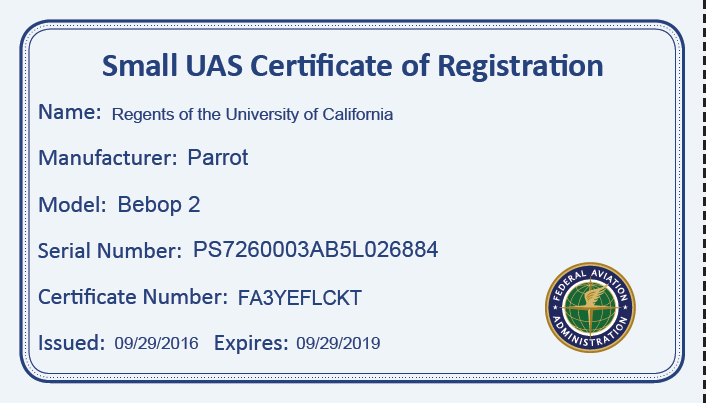
\includegraphics[width=0.5\linewidth]{images/reg_cert} 

}

\caption{Example UAS Registration Certificate}\label{fig:reg-cert}
\end{figure}

All UAS that weigh between 0.55 lbs and 55 lbs (under 14 CFR 48) must be registered online at \url{https://faadronezone.faa.gov/}.

UAS that weigh more than 55 lbs or are required to have UAS registration that is valid internationally must be registered under 14 CFR 47 and must be done through mail with an Original Aircraft Registration Form, AC Form 8050-1.

\hypertarget{registration-of-model-aircraft}{%
\section{Registration of Model Aircraft}\label{registration-of-model-aircraft}}

Model Aircraft are required to be registered under 14 CFR 48. Though typically most UAS owned by the UC will be registered individually, there are some cases where they may be registered as MA.

\begin{quote}
In general, UAS that are used exclusively as model aircraft may be registered as a group under the owner of the model aircraft. In the case of the group or company owned model aircraft, they may be registered under the primary user or manager of the model aircraft as the model aircraft registration is not considered proof of ownership.
\end{quote}

\textbf{Common Scenarios for Model Aircraft}

\begin{itemize}
\tightlist
\item
  Model Aircraft owned by students should be registered by the student
\item
  Model Aircraft owned by a student club can be registered by a member of the student club, a club mentor or faculty adviser.
\item
  Model Aircraft used in classroom or educational activity should have the faculty, instructor or department staff member register for an FAA registration number to be placed on all aircraft.
\end{itemize}

\hypertarget{record-keeping-policy-requirements}{%
\section{Record Keeping Policy Requirements}\label{record-keeping-policy-requirements}}

Records of UC-owned UAS registration must be provided to the designated local authority or the systemwide designated authority. Registration of all unmanned aircraft used for University business must be provided to the designated local authority or the systemwide designated authority. UC Drones may be used to submit records electronically and other electronic submission processes may be available in the future. A University location may additionally implement a centralized registration process using a single FAA online account.

\hypertarget{fraudulent-drone-registration-websites}{%
\section{Fraudulent Drone Registration Websites}\label{fraudulent-drone-registration-websites}}

Unfortunately, there are several fraudulent websites that advertise Drone registration. The only registration site is at \url{https://faadronezone.faa.gov/} and registration only costs \$5 per aircraft. UAS registration through the FAA's website requires you to create an account with the FAA, but is otherwise instantaneous. Any website that offers to register an aircraft on your behalf, or offers an `enhanced' or `expedited' registration is fraudulent. The correct website looks as in Figure \ref{fig:reg-page}

\begin{figure}

{\centering 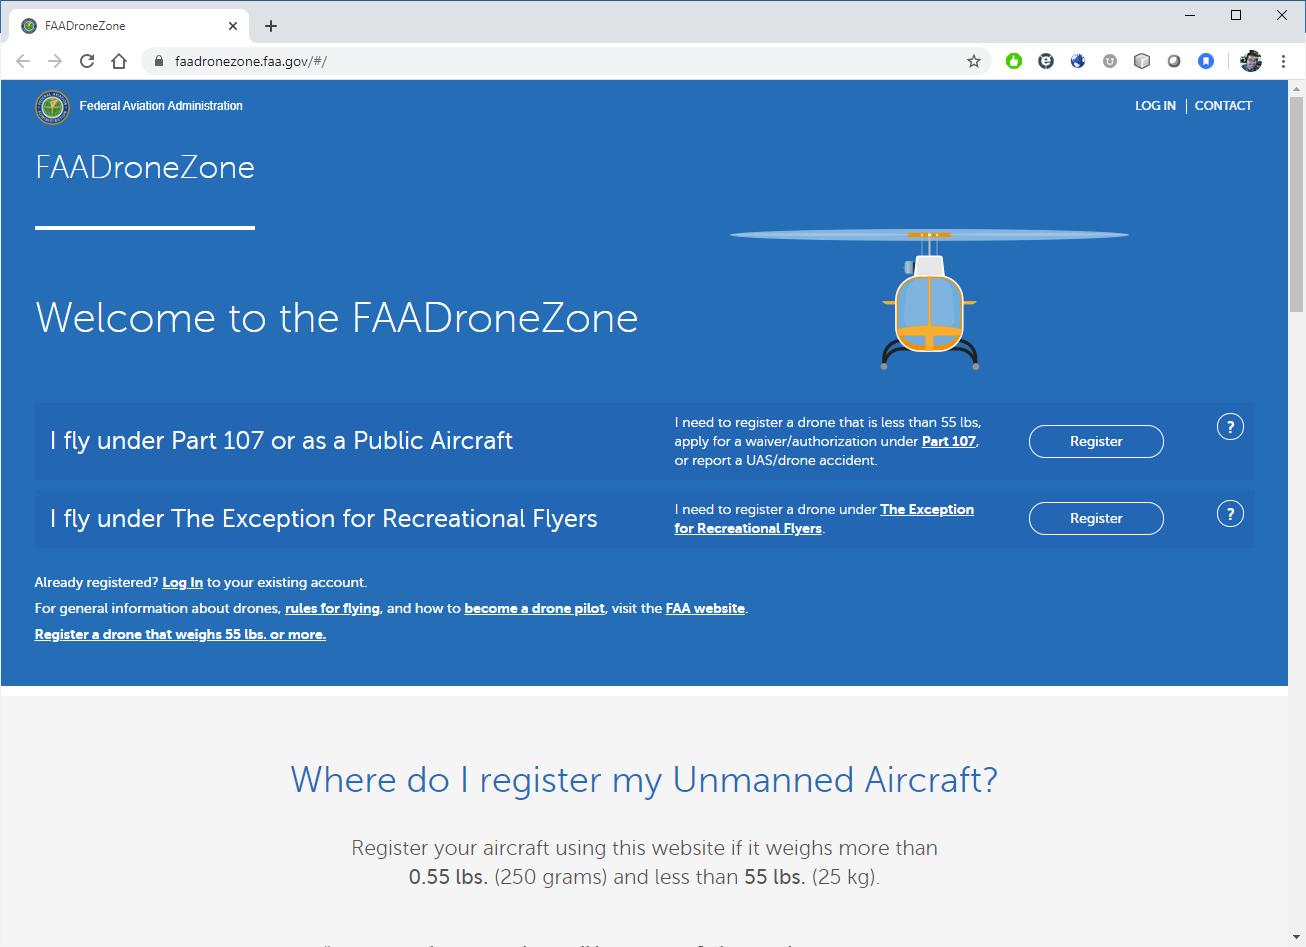
\includegraphics[width=0.8\linewidth]{images/reg_site} 

}

\caption{FAA DroneZone}\label{fig:reg-page}
\end{figure}

\hypertarget{ch-review}{%
\chapter{Review of UAS Activity}\label{ch-review}}

\hypertarget{s-general}{%
\section{General Procedures}\label{s-general}}

The \protect\hyperlink{FR}{Flight Request} process provides the University of California the ability to validate whether the proposed use complies with the Policy that requires all operations are performed in a manner that mitigates risks to safety, security, privacy and ensures compliance with any applicable regulation. All persons seeking to operate a UAS covered within the Policy must submit a \protect\hyperlink{FR}{UAS Request Form} to the \protect\hyperlink{DLA}{Designated Local Authority} or \protect\hyperlink{SDA}{Systemwide Designated UAS Authority} if a \protect\hyperlink{DLA}{Designated Local Authority} has not been appointed for a \protect\hyperlink{UL}{University Location}.

The Policy requires that the review of a proposed operation must be responded to within two weeks.

Approvals for \protect\hyperlink{UASactivity}{UAS activity} may be granted in many forms:

\begin{itemize}
\tightlist
\item
  Single or set of UAS flights during a specific time-window
\item
  Set of UAS flights over a defined period of time
\item
  Scheduled recurrent UAS flights at a defined location
\item
  Unscheduled UAS usage at a series of predefined locations
\item
  Standing approvals
\end{itemize}

Records of approval and the terms of the approval must be kept by the \protect\hyperlink{DLA}{Designated Local Authority} and the \protect\hyperlink{SDA}{Systemwide Designated UAS Authority}.

\hypertarget{s-form}{%
\section{Submission of UAS Request Form}\label{s-form}}

The \protect\hyperlink{FR}{UAS Request Form} is a documented request of UAS activity. An example form can be made available by a \protect\hyperlink{DLA}{Designated Local Authority} or \protect\hyperlink{SDA}{Systemwide Designated UAS Authority} (Figure \ref{fig:nice-fig2}). The Policy does not mandate a specific form or system for submitting a \protect\hyperlink{FR}{UAS Request Form}. UC Risk and Safety Solutions has developed UC Drones \protect\hyperlink{FR}{UAS Request Form} as a means to standardize request information and is available for all UC campuses (More information on UC Drones in Section \ref{sec-UCDrones}). A \protect\hyperlink{UL}{University Location} may also establish a specialized for any \protect\hyperlink{UASactivity}{UAS activity} as long as it collects sufficient information to conduct a review of the \protect\hyperlink{UASactivity}{UAS activity} to ensure Policy compliance (Figure \ref{fig:flight-request-ucsd}).

\begin{figure}

{\centering 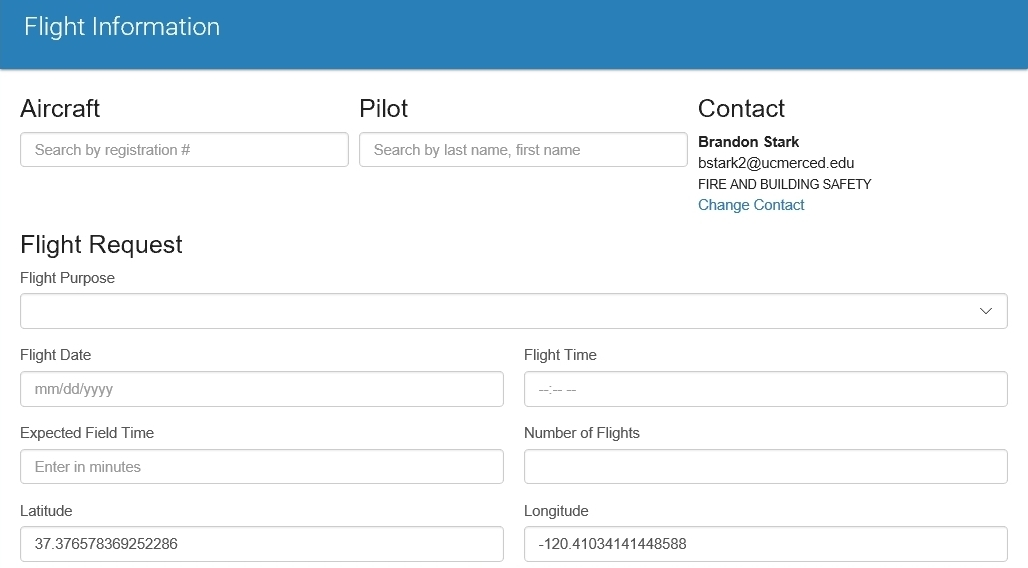
\includegraphics[width=0.5\linewidth]{images/flight_request1} 

}

\caption{Example UAS Flight Request Form - UC Drones}\label{fig:nice-fig2}
\end{figure}

\begin{figure}

{\centering 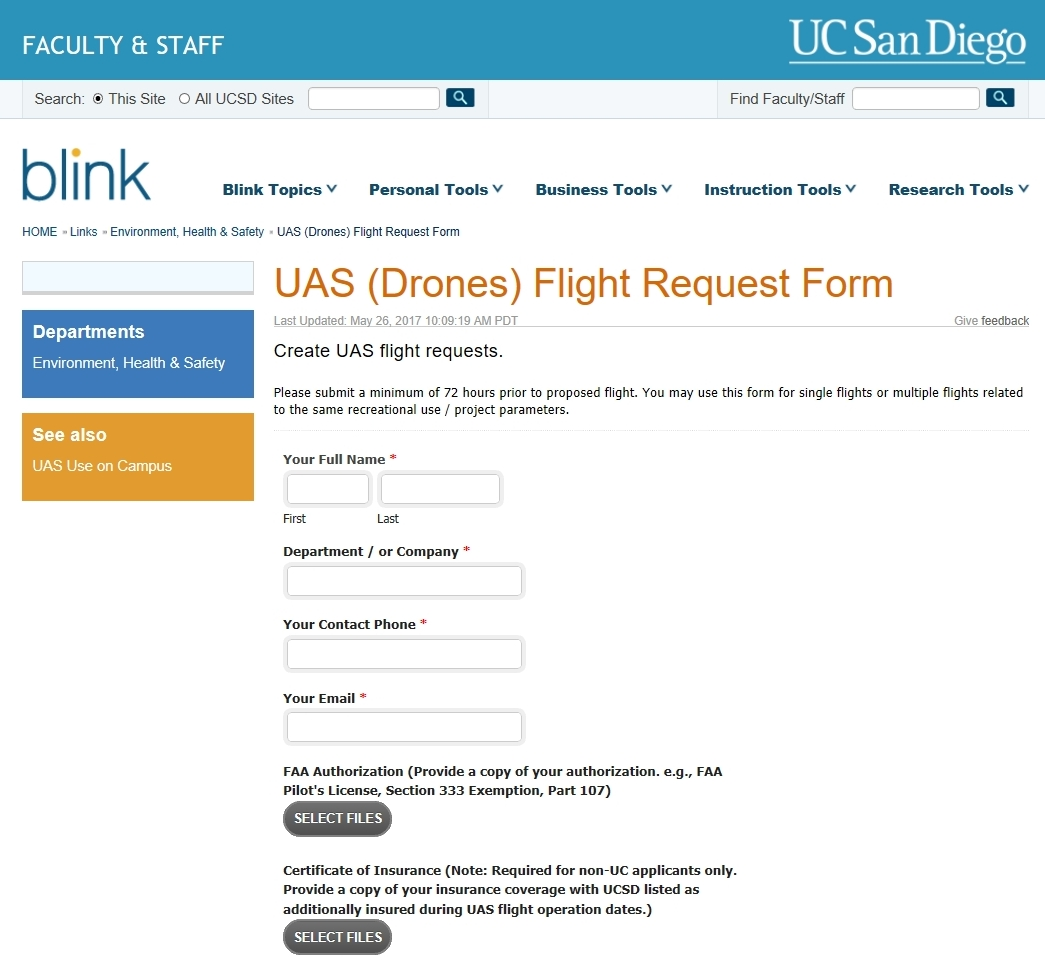
\includegraphics[width=0.5\linewidth]{images/flight_request2} 

}

\caption{Example UAS Flight Request Form - UCSD}\label{fig:flight-request-ucsd}
\end{figure}

\hypertarget{s-reviewer}{%
\section{Reviewer of UAS Activity}\label{s-reviewer}}

The Policy grants authority to review \protect\hyperlink{UASactivity}{UAS activity} to the \protect\hyperlink{SDA}{Systemwide Designated UAS Authority} and the \protect\hyperlink{DLA}{Designated Local Authority}. Per the Policy, the \protect\hyperlink{SDA}{Systemwide Designated UAS Authority} may review \protect\hyperlink{UASactivity}{UAS activity} unless a \protect\hyperlink{DLA}{Designated Local Authority} is assigned to review \protect\hyperlink{UASactivity}{UAS activity} at a campus. In many cases, the \protect\hyperlink{DLA}{Designated Local Authority} is in a better position to evaluate the safety and impacts to privacy of \protect\hyperlink{UASactivity}{UAS activity} on their location.

As per the relationship between the \protect\hyperlink{SDA}{Systemwide Designated UAS Authority} and \protect\hyperlink{DLA}{Designated Local Authority}, the \protect\hyperlink{SDA}{Systemwide Designated UAS Authority} will provide interpretation of regulations, including international, federal, state and local, and provide subject matter expertise to the \protect\hyperlink{DLA}{Designated Local Authority} to pass the final judgment. It is expected that as campuses become more familiar with UAS regulations and their use, the majority of use cases may be handled completely by the \protect\hyperlink{DLA}{Designated Local Authority}.

A \protect\hyperlink{LSP}{location specific policy or procedure} may further establish the role of the \protect\hyperlink{DLA}{Designated Local Authority} and other campus entities that may be granted autonomy to review \protect\hyperlink{UASactivity}{UAS activity}.

\hypertarget{s-ecrit}{%
\section{Criteria Used to Evaluate UAS Activity}\label{s-ecrit}}

The Policy mandates that all \protect\hyperlink{UASactivity}{UAS activity} within the scope of the policy must be approved prior to flight. The review process must include:

\begin{itemize}
\tightlist
\item
  Review of compliance with applicable regulations (Section \ref{ss-regcomp}) and includes Export Control (Section \ref{ss-expcon}).
\item
  Review of impacts to safety (Section \ref{ss-safety}).
\item
  Review of impacts to privacy, civil rights and liberties (Section \ref{ss-privacy}).
\item
  Review of insurance (Section \ref{ss-insrnc}).
\end{itemize}

The review process may additionally include

\begin{itemize}
\tightlist
\item
  Prioritization of \protect\hyperlink{UB}{University Business}
\item
  Approval of facility manager or other local authority
\item
  Approval or consent of persons that may be impacted by the proposed operation
\item
  Previous documented flight experience or expertise
\item
  Impacts to wildlife or other environmental concerns
\end{itemize}

\hypertarget{ss-regcomp}{%
\subsection{Evaluation of Regulatory Compliance}\label{ss-regcomp}}

UAS regulations are regularly evolving; there are multiple legal pathways within the US and internationally. The Policy does not mandate exclusive compliance with a particular set of regulations. The \protect\hyperlink{SDA}{Systemwide Designated UAS Authority} is responsible for providing the interpretation to regulations for the \protect\hyperlink{DLA}{Designated Local Authority}.

\textbf{Civil Regulations for Small Unmanned Aircraft Systems (14 CFR 107)} - A large portion of UAS activity within the UC system falls under the recently released regulations in 14 CFR 107. There are 22 points of compliance as outlined in the 14 CFR 107 compliance list found in Section \ref{s-part107}. If further regulations are issued that provide alternative legal pathways, they may be utilized without requiring modification to policy. By default within the United States, all UAS operations in the \protect\hyperlink{NAS}{NAS} are regulated under 14 CFR 107 unless it meets the exception criteria for limited exception for recreational purposes, \protect\hyperlink{PAO}{PAO} or with a Section 333 Exemption.

\textbf{Exception for Limited Recreational Operations of Unmanned Aircraft} - UAS activity may be exempt from 14 CFR 107 regulations if the flight operations complies with the exception for limited recreational operations of unmanned aircraft as described in 49 USC 44809. While this typically covers recreational activity, in specific situations academic research and coursework may also be covered. More information can be found in Section \ref{s-recreation}.

\textbf{Public Agency Operations (14 CFR 91)} - UAS activity may be conducted under 14 CFR 91 regulations when classified as a \protect\hyperlink{PAO}{Public Agency Operation} with a \protect\hyperlink{PA}{Public Aircraft}. UAS activity requested as an \protect\hyperlink{PAO}{Public Agency Operation} should be reviewed on a case-by-case basis as these authorizations are often specific to an aircraft, location, purpose and organization, and may contain special restrictions or allowances. The \protect\hyperlink{SDA}{Systemwide Designated UAS Authority} is available to review and issue an interpretation for compliance.

\textbf{Section 333 Exemptions (14 CFR 91)} - UAS activity may be conducted under 14 CFR 91 regulations through a special exemption known as Section 333 Exemption (Section 333 of Public Law 112-95). Operations conducted through Section 333 exemptions should be reviewed on a case-by-case basis as these authorizations contain different restrictions and allowances, depending on use case.

\textbf{International Regulations} - UAS activity conducted outside of the US are subject to the host country's regulations. The \protect\hyperlink{SDA}{Systemwide Designated UAS Authority} maintains a database of international UAS regulations and will provide an interpretation of regulations as requested.

\textbf{State or Local Regulations} - Many states and cities have begun to implement local authority over \protect\hyperlink{UASactivity}{UAS activity}. There is currently no central database of such regulations, so these must be identified and reviewed on a case-by-case basis. The \protect\hyperlink{SDA}{Systemwide Designated UAS Authority} maintains a database of common state and local regulations requested by UC \protect\hyperlink{UASactivity}{UAS activity}. While the \protect\hyperlink{FAA}{FAA} maintains sole jurisdiction of the \protect\hyperlink{NAS}{NAS}, state and local authorities may enact regulations related to traditional police powers such as land use planning and zoning, health, safety and advertising.

\hypertarget{ss-expcon}{%
\subsection{Evaluation of Compliance with Export Control}\label{ss-expcon}}

Certain UAS may be export controlled under US Export Regulations and, as such, may not be physically exported outside the United States without a license from the US government. In addition, a license may be required if foreign nationals located within the US are provided access to the technology related to such systems (deemed exports). All UC individuals or organizations that intend to design, build, research, use in research, modify, dismantle, and/or operate a UAS in foreign countries and/or with foreign nationals in the US or abroad must do so in accordance with the Export regulations and the UC Export Control Policy. Documentation of UC-owned unmanned aircraft is additionally available for Export Control personnel to review.

\hypertarget{ss-safety}{%
\subsection{Evaluation of Impacts with Safety}\label{ss-safety}}

The review of the \protect\hyperlink{UASactivity}{UAS activity} is limited to the scope of campus or public safety. It does not review all safety implications.

As applicable, the \protect\hyperlink{DLA}{Designated Local Authority} or \protect\hyperlink{SDA}{Systemwide Designated UAS Authority} should review for

\begin{itemize}
\item
  Mitigation strategies for

  \begin{itemize}
  \tightlist
  \item
    Pedestrian Safety
  \item
    Vehicular Safety
  \item
    Loss of Control
  \end{itemize}
\item
  Crowd Control
\item
  Sensitive Locations
\end{itemize}

Not all \protect\hyperlink{UASactivity}{UAS activity} will require a detailed review for minor or low risk activity. A primary means of mitigation for safety impacts is to relocate \protect\hyperlink{UASactivity}{UAS activity} to large, open areas away from non-participating persons.

The review of safety does not absolve the \protect\hyperlink{RPIC}{RPIC}'s responsibility to maintain a safe operating environment. The safety aspect of the review does not consider:

\begin{itemize}
\tightlist
\item
  Weather conditions
\item
  Obstructions from ground hazards (Trees, temporary structures)
\item
  Previous unrecorded flight experience
\end{itemize}

\hypertarget{ss-privacy}{%
\subsection{Evaluation of Impacts with Privacy, Civil Rights and Liberties}\label{ss-privacy}}

The use of UAS is still relatively new and there is still much trepidation regarding privacy, civil rights, liberties and UAS. Compliant with other UC policies regarding privacy, \protect\hyperlink{UASactivity}{UAS activity} must respect the privacy of others and not infringe on their civil rights and liberties.

The perceived invasion of privacy is additionally to be avoided. It is unlikely that a proponent would blatantly propose activity that would invade a person's privacy. However, there may be proposed activity that may be perceived as potentially invading privacy. An example of this would be in \protect\hyperlink{UASactivity}{UAS activity} in close proximity to residential buildings. Regardless of the intent or business nature of the \protect\hyperlink{UASactivity}{UAS activity}, unless mitigating strategies are employed, such activities should be prohibited. Best practices regarding \protect\hyperlink{UASactivity}{UAS activity} are listed in Chapter \ref{ch-privacy}.

\hypertarget{ss-insrnc}{%
\subsection{Evaluation of Compliance with Insurance}\label{ss-insrnc}}

All \protect\hyperlink{UASactivity}{UAS activity} must be covered by liability insurance. The UC provides automatic coverage for \protect\hyperlink{UASactivity}{UAS activity} for UC-owned \protect\hyperlink{UA}{Unmanned Aircraft}. Additionally, personally owned \protect\hyperlink{UA}{Unmanned Aircraft} used for \protect\hyperlink{UB}{University Business} can be covered if the \protect\hyperlink{UASactivity}{UAS activity} is approved.

All \protect\hyperlink{rdparty}{3\textsuperscript{rd} Party} \protect\hyperlink{UASactivity}{UAS activity} must submit appropriate insurance, including a written agreement which indemnifies and holds the University harmless from any resulting claims or harm to individuals and damage to University property.

More details are provided in Chapter \ref{ch-insurance}.

\hypertarget{s-factors}{%
\section{Other Factors}\label{s-factors}}

At a minimum, the above criteria are necessary to be reviewed. However, there may be other factors that may be utilized at the discretion of a \protect\hyperlink{DLA}{Designated Local Authority} in accordance with a \protect\hyperlink{LSP}{location specific policy or procedure}.\\
This may include but is not limited to:

\begin{itemize}
\tightlist
\item
  Prioritization of \protect\hyperlink{UB}{University Business}.
\item
  \protect\hyperlink{riskscore}{Risk Score} of \protect\hyperlink{UASactivity}{UAS activity}.
\item
  Approval of facility manager or other local authority.
\item
  Approval or consent of persons that may be impacted by the proposed operation.
\item
  Previous documented flight experience or expertise.
\item
  Impacts to wildlife or other environmental concerns.
\end{itemize}

There are currently only limited existing standards for \protect\hyperlink{UASactivity}{UAS activity} that may or may not be applicable within the UC system. A \protect\hyperlink{LSP}{location specific policy or procedure} may elect to adopt standards as they are developed. It is intended that the \protect\hyperlink{SDA}{Systemwide Designated UAS Authority} will continue to evaluate and provide recommendations for specific standards.

\hypertarget{s-rp}{%
\section{Relationship of a UC Review Process with Applicable Regulations}\label{s-rp}}

The University of California requires that all \protect\hyperlink{UASactivity}{UAS activity} comply with all applicable regulations, at the international, federal, state and local levels, as well as mitigates risks to safety, security and privacy. Additionally, a \protect\hyperlink{DLA}{Designated Local Authority} may choose to review other factors.

It is foreseeable that otherwise legal UAS activity may be prohibited or require modification by either the \protect\hyperlink{DLA}{Designated Local Authority} or \protect\hyperlink{SDA}{Systemwide Designated UAS Authority}.

Example of potential scenarios:

\begin{itemize}
\tightlist
\item
  Non-essential \protect\hyperlink{UASactivity}{UAS activity} in the vicinity of dorms where privacy concerns exist.
\item
  \protect\hyperlink{UASactivity}{UAS activity} where the use of a UAS would disrupt other \protect\hyperlink{UB}{University Business} such as commencement ceremonies or campus events.
\item
  Proposed \protect\hyperlink{UASactivity}{UAS activity} that conflict with other previously approved \protect\hyperlink{UASactivity}{UAS activity}.
\item
  Proposed \protect\hyperlink{UASactivity}{UAS activity} that is likely to violate \protect\hyperlink{FAA}{FAA} regulations such as direct flyovers of large areas of a busy campus.
\item
  Proposed \protect\hyperlink{UASactivity}{UAS activity} requires the reservation of an athletics field that is occupied.
\item
  Proposed \protect\hyperlink{UASactivity}{UAS activity} is above a preferred flight altitude limit for a specific location and may interfere with medical helicopter activity.
\end{itemize}

The review by a \protect\hyperlink{DLA}{Designated Local Authority} or \protect\hyperlink{SDA}{Systemwide Designated UAS Authority} also includes state or local regulations at sites such as California State Parks or County Park Systems. A \protect\hyperlink{UASactivity}{UAS activity} may be considered legal under \protect\hyperlink{FAA}{FAA} regulations, but may be prohibited by other regulations, and thus would not be approved. Due to the vast diversity of regulations at the state and local level, a review process may take longer at those sites.

\hypertarget{s-term-approval}{%
\section{Terms of Approval}\label{s-term-approval}}

In some cases, \protect\hyperlink{UASactivity}{UAS activity} approval may require additional terms or conditions. These may arise from \protect\hyperlink{UASactivity}{UAS activity} where additional flexibility is requested, such as recurrent \protect\hyperlink{UASactivity}{UAS activity} in a low-risk location. The \protect\hyperlink{DLA}{Designated Local Authority} or \protect\hyperlink{SDA}{Systemwide Designated UAS Authority} may attach additional requirements or procedures at their discretion.

Items to consider as part of the Terms of Approval

\begin{itemize}
\tightlist
\item
  Frequency of reporting.
\item
  \protect\hyperlink{currency}{Currency} requirements of the \protect\hyperlink{RPIC}{RPIC}.
\item
  Procedures to address rescheduling.
\item
  Procedures for accident notification.
\end{itemize}

Example language that may be used in Terms of Approval can be found in Chapter \ref{ch-example-terms}.

\hypertarget{ch-reporting}{%
\chapter{UAS Activity Reporting}\label{ch-reporting}}

The (ref:uaspostlight) of \protect\hyperlink{UASactivity}{UAS activity} is an important aspect of oversight, management and the development of future policies and procedures. The Policy mandates that post-flight reporting must be accomplished but does not specify details regarding the frequency or specific information requirements. This section provides guidance on establishing a successful reporting system.

All reporting must meet or exceed compliance with all applicable regulations and policies. Currently, the UC has 5 UAS specific reporting compliance obligations. The UC additionally has other reporting compliance obligations related to workplace safety and accident reporting.

\hypertarget{s-reporting-compliance}{%
\section{UAS Reporting Compliance Obligations}\label{s-reporting-compliance}}

\begin{itemize}
\tightlist
\item
  All \protect\hyperlink{UASactivity}{UAS activity} covered under the UC's UAS insurance must be reported to the insurance broker on a quarterly basis.
\item
  All \protect\hyperlink{UASactivity}{UAS activity} classified as a \protect\hyperlink{PAO}{PAO} must be reported to the FAA on a monthly basis.
\item
  Records of \protect\hyperlink{UASactivity}{UAS activity} conducted under 14 CFR 107 may be requested by the \protect\hyperlink{FAA}{FAA} and must be made available.
\item
  All \protect\hyperlink{UASactivity}{UAS activity} conducted under a systemwide \protect\hyperlink{FAA}{FAA} \protect\hyperlink{AA}{Airspace Authorization}, \protect\hyperlink{AW}{Airspace Waiver} or \protect\hyperlink{COA}{COA} must be documented and made available to the \protect\hyperlink{FAA}{FAA} upon request.
\item
  Any incident subject to \protect\hyperlink{FAA}{FAA} or NTSB reporting requirements
\item
  Any incident subject to CalOSHA reporting requirements
\end{itemize}

\hypertarget{s-safety-metric-tracking}{%
\section{UAS Safety Metric Tracking}\label{s-safety-metric-tracking}}

An important aspect of regular \protect\hyperlink{UASactivity}{UAS activity} reporting is the tracking of safety metrics. Through the use of effective data collection, trends regarding UAS safety enables \protect\hyperlink{DLA}{Designated Local Authorities} to identify and make recommendations to adjust local procedures without compromising safety.

Flight record statistics may also be utilized for reviews for high \protect\hyperlink{riskscore}{Risk Score} activity. Example scenarios include standing approval for media representatives who must maintain \protect\hyperlink{currency}{currency} for \protect\hyperlink{UASactivity}{UAS activity} that require a higher level of expertise due to a higher \protect\hyperlink{riskscore}{Risk Score}.

The \protect\hyperlink{AB}{UAS Advisory Board} additionally reviews all \protect\hyperlink{UASactivity}{UAS activity} reporting for its analysis on the effectiveness of the Policy.

\hypertarget{s-UAS-activity-reports}{%
\section{Collection of UAS Activity Reports}\label{s-UAS-activity-reports}}

The Policy does not mandate a specific process for collection of a (ref:UASpostflight). A \protect\hyperlink{DLA}{Designated Local Authority} or \protect\hyperlink{LSP}{location specific policy or procedure} may opt to implement a different solution, depending on need or desired data. It is recommended that \protect\hyperlink{postflight}{Post-Flight Reports} be collected as immediately as possible from the proponent to minimize complacency and forgotten minor incidents.

Example Post Flight Report Collection

\begin{itemize}
\tightlist
\item
  \protect\hyperlink{UCDrones}{UC Drones} on a per day, per aircraft, per pilot basis.
\item
  Excel spreadsheet of reports collected on a weekly basis.
\item
  Webform generated report.
\item
  Electronic submission via access to a commercial cloud solution.
\item
  Scanned handwritten documents.
\end{itemize}

The webapp \protect\hyperlink{UCDrones}{UC Drones} provides \protect\hyperlink{DLA}{Designated Local Authorities} with a mechanism to collect and review \protect\hyperlink{UASactivity}{UAS activity} reports (See Section \ref{sec-UCDrones}). Data entered in \protect\hyperlink{UCDrones}{UC Drones} may be made available to authorized personnel in compliance with UC policies.

\hypertarget{s-minimum-reporting}{%
\section{UC Minimum Reporting Guidance}\label{s-minimum-reporting}}

Flight record data must include sufficient information to be able to determine:

\begin{itemize}
\tightlist
\item
  Date
\item
  Pilot
\item
  Aircraft
\item
  Location
\item
  Number of flights
\item
  Total flight time
\item
  Accident or incident records
\end{itemize}

Flight records may additionally include

\begin{itemize}
\tightlist
\item
  Flight altitude or distance
\item
  Telemetry data
\item
  Fuel or Battery information
\item
  Software/hardware configurations, including payload
\item
  Weather conditions
\item
  Images or other media of the \protect\hyperlink{UASactivity}{UAS activity}
\end{itemize}

\hypertarget{s-3rdparty-reporting}{%
\section{3rd Party Reporting}\label{s-3rdparty-reporting}}

UAS activity accomplished by a \protect\hyperlink{rdparty}{3\textsuperscript{rd} Party} must be tracked and monitored. Failure to submit records may be considered in future \protect\hyperlink{UASactivity}{UAS activity} review.

\hypertarget{s-AMOC}{%
\section{Alternative Means of Compliance}\label{s-AMOC}}

In some use cases, it may be unfeasible to collect accurate flight record information.

Example scenarios:

\begin{itemize}
\tightlist
\item
  Indoor Activity
\item
  Individual Recreational Model Aircraft
\item
  Coursework with large groups of students
\end{itemize}

In these cases, the \protect\hyperlink{LSP}{location specific policy or procedure} or \protect\hyperlink{DLA}{Designated Local Authority}, in consultation with the \protect\hyperlink{SDA}{Systemwide Designated UAS Authority} and or the \protect\hyperlink{AB}{UAS Advisory Board} may develop alternative means of compliance. Example solutions include low fidelity usage approximations on a daily or monthly summary.

\hypertarget{ch-nonreprisal}{%
\chapter{Non-Punative Reporting Statement}\label{ch-nonreprisal}}

It is recognized that humans will make errors, accidents happen, and systems must be developed that are error tolerant and behaviors changed to lessen the chance of errors occuring. It is not the goal of the Policy to authorize the \protect\hyperlink{SDA}{Systemwide Designated UAS Authority} or \protect\hyperlink{DLA}{Designated Local Authorities} to seek out someone who has reported an error, accident, or mishap in order to administer retribution. All communications made by persons abiding by the UAS reporting requirements shall be made with the assurance that no retaliation or reprisal shall occur.

Upon the submission of a report describing an error, incident or accident, the \protect\hyperlink{SDA}{Systemwide Designated UAS Authority} or \protect\hyperlink{DLA}{Designated Local Authority} may reach out to the reporter for followup and clarification. It is important to note that the goal is not to punish, but to ensure it does not happen again.

\hypertarget{ch-accidents}{%
\chapter{UAS Accident Reporting}\label{ch-accidents}}

All UAS accidents, incidents and malfunctions must be reported. This differs from \protect\hyperlink{FAA}{FAA} requirements under 14 CFR 107 because the UC has other reporting compliance obligations that it must meet. A \protect\hyperlink{DLA}{Designated Local Authority} or the \protect\hyperlink{SDA}{Systemwide Designated UAS Authority} will make a determination if the accident, incident or malfunction requires further reporting with the appropriate regulatory body.

In data collected from September 2016 to March 2018, UAS accidents, incidents or malfuctions that resulted in non-minor UAS damage, injury or property damage were caused by evenly between human-factors or system malfunctions.

\hypertarget{s-common-accidents}{%
\section{Common Accidents, Incidents or Malfunctions}\label{s-common-accidents}}

Some of common UAS accidents, incidents and malfunctions that have been reported include:

\begin{itemize}
\tightlist
\item
  Operator error resulting in collision with stationary object
\item
  Loss of Battery/Fuel
\item
  Fly-away/loss of control
\item
  Hardware malfunctions such as GPS interference
\item
  Improper `Return to Launch' location
\item
  Improper assembly of vehicle
\item
  Experimental hardware/software
\item
  Hazardous weather conditions
\item
  Battery caught fire from puncture or impact
\end{itemize}

\hypertarget{s-reporting-exemptions}{%
\section{Exemptions}\label{s-reporting-exemptions}}

The following accidents, incidents and malfunctions are exempt from mandatory reporting, but are still welcome in post flight reports

\begin{itemize}
\tightlist
\item
  Malfunctions related to payloads that have no impact on safety
\item
  Damage of components designed or expected to fail during regular use
\item
  Rough or hard landings that do not result in damage
\item
  Damage to the drone due to improper ground-handling/transportation
\end{itemize}

\hypertarget{s-near-misses}{%
\section{Near Misses}\label{s-near-misses}}

A near miss, also known as a close call or near hit, is defined as an unplanned event that did not result in injury or damage -- but had the potential to do so. Typically, these events result from either unsafe conditions, arising from the work environment itself, or unsafe acts, arising from UAS activities. Reporting a near-miss can ensure that future incidents and injuries are avoided.

Example Near-Misses

\begin{itemize}
\tightlist
\item
  Insufficient hazard analysis from utilizing out of date satelite imagery
\item
  Interations with non-participants or unaware university officials
\item
  Interactions with wildlife
\item
  Battery draining faster than normal
\end{itemize}

\hypertarget{s-investigation}{%
\section{Accident Investigation}\label{s-investigation}}

The \protect\hyperlink{DLA}{Designated Local Authority} or \protect\hyperlink{SDA}{Systemwide Designated UAS Authority} may initiate an investigation of a reported accident, incident, malfunction or reported near-miss situation. Any opportunity to better understand the root cause of a UAS accident is valuable. A process or procedure for accident investigation may be written into a \protect\hyperlink{LSP}{location specific policy or procedure}. Below are some general guidelines for conducting a UAS Accident Investigation (adapted from OSHA).

\hypertarget{incident-investigation-principles}{%
\subsection{Incident Investigation Principles}\label{incident-investigation-principles}}

\begin{itemize}
\tightlist
\item
  Do not assign blame to the reporter
\item
  Remind everyone that the investigation is to learn and prevent, not to penalize
\item
  Ensure everyone's narrative is heard
\end{itemize}

\hypertarget{process}{%
\subsection{Process}\label{process}}

\begin{itemize}
\item
  Call or gather the necessary persons to conduct the investigation
\item
  Identify and gather witnesses (if applicable)
\item
  Collect facts
\item
  Collect a narrative from the \protect\hyperlink{RPIC}{RPIC} and witnesses
\item
  Document the incident with photos and videos (if applicable)
\item
  Complete a report (if applicable)

  \begin{itemize}
  \tightlist
  \item
    Identify causes
  \item
    Identify latent conditions
  \item
    Identify corrective actions
  \end{itemize}
\end{itemize}

\hypertarget{interviewing-people}{%
\subsection{Interviewing People}\label{interviewing-people}}

\begin{itemize}
\tightlist
\item
  Use open-ended questions
\item
  State the purpose of the investigation is fact-finding, not fault-finding
\item
  Ask the individual to recount their version of the event
\item
  Ask clarifying questions to fill missing information
\item
  Ask the individual what they think could have prevented the incident, focusing on the conditions and events preceding the event.
\end{itemize}

\hypertarget{information-to-collect}{%
\subsection{Information to Collect}\label{information-to-collect}}

\begin{itemize}
\item
  \protect\hyperlink{RPIC}{RPIC} information
\item
  UAS information, including

  \begin{itemize}
  \tightlist
  \item
    Hardware or Software firmware
  \item
    Automated features of the \protect\hyperlink{UA}{Unmanned Aircraft} used
  \end{itemize}
\item
  Time of Day
\item
  Location
\item
  Potential visual obstructions, including

  \begin{itemize}
  \tightlist
  \item
    Trees,
  \item
    Powerlines,
  \item
    People or crowds,
  \end{itemize}
\item
  Weather conditions, such as

  \begin{itemize}
  \tightlist
  \item
    Wind
  \item
    Sun location
  \item
    Clouds or Fog
  \end{itemize}
\item
  Supervisor information
\item
  Potential witnesses
\item
  Corrective actions
\item
  Causal factors that may have played a role
\end{itemize}

\hypertarget{determining-causal-factors}{%
\subsection{Determining Causal Factors}\label{determining-causal-factors}}

Causal factors for an accident are rarely definitive and may be subjective. Some example causal factors to investigate include, but are not limited to:

\begin{itemize}
\item
  Was there external pressures that may have contributed to the incident, such as weather, pressure from management, time-limits, etc?
\item
  Was the location a contributing factor?
\item
  Was the management or oversight procedures a contributing factor?

  \begin{itemize}
  \tightlist
  \item
    Consider administrative or engineering factors
  \end{itemize}
\item
  Was equipment questionable but still used?
\item
  Was there a miscommunication within the operating team?
\item
  Were there any quick fixes/unplanned changes made in the field to complete the mission?
\end{itemize}

\hypertarget{ch-insurance}{%
\chapter{UAS Insurance}\label{ch-insurance}}

\hypertarget{s-UC-liability}{%
\section{Liability Coverage}\label{s-UC-liability}}

The University of Calfironia has purchased an \protect\hyperlink{UA}{Unmanned Aircraft} Liability Policy. This policy has a total of \$5 Mil limit with a \$1 Mil Personal Injury sublimit and \$1 Mil Products/Completed Operations sublimit.

Coverage is automatic for \protect\hyperlink{UASactivity}{UAS activity} that meet the following criteria:

\begin{itemize}
\tightlist
\item
  Flight operations are conducted on behalf and sanctioned by the University of California.
\item
  Aircraft weight under 55 lbs (at time of takeoff)
\item
  Flight operations are within \protect\hyperlink{VLOS}{VLOS}
\item
  Flight operations are below 400 ft above ground level.
\item
  Flight operations must be conducted within the United States.
\end{itemize}

Any \protect\hyperlink{UASactivity}{UAS activity} that do not meet the above criteria or operate outside the above criteria must be reported to and approved by the insurance underwriter in order to be covered.

Any \protect\hyperlink{UASactivity}{UAS activity} that is not approved by a \protect\hyperlink{DLA}{Designated Local Authority} or \protect\hyperlink{SDA}{Systemwide Designated UAS Authority} is not covered by this liability insurance coverage.

\hypertarget{ss-personally-owned-UAS-coverage}{%
\subsection{Personally Owned Unmanned Aircraft Used for University Business}\label{ss-personally-owned-UAS-coverage}}

The University of California has extended their UAS liability policy to enable coverage of UAS owned by UC students, staff or faculty used for \protect\hyperlink{UB}{University Business}, including research. Coverage in contingent on compliance with the policy and procedures on UAS usage. This coverage is not intended to cover student organizations or (ref:rdParty vendors or contractors.

\hypertarget{ss-campus-police-coverage}{%
\subsection{Coverage for Campus Police}\label{ss-campus-police-coverage}}

The University of California has extended their UAS liability policy to enable coverage of UAS by Campus Police. All coverage is contingent on the \protect\hyperlink{UASactivity}{UAS activity} being sanctioned by the UC.

Any \protect\hyperlink{UASactivity}{UAS activity} that is not approved by a \protect\hyperlink{DLA}{Designated Local Authority} or \protect\hyperlink{SDA}{Systemwide Designated UAS Authority} is not covered by this liability insurance.

\hypertarget{s-UC-physical-damage}{%
\section{Physical Damage Coverage}\label{s-UC-physical-damage}}

Physical damage to a UAS is covered under a blanket policy issued by the University's captive insurance company, Fiat Lux Risk and Insurance Company

\begin{itemize}
\tightlist
\item
  Coverage applies in flight only when an approved flight plan is filed in accordance with UC UAS Policy, including the UC Drone web app or other means of compliance.\\
\item
  Coverage is limited to \$25,000 for Unmanned Aircrafts
\item
  Payload is covered separately and not included within this limit
\item
  \$1,000 deductible applies to each and every loss (including payload)
\item
  Coverage additionally applies in the event of theft, vandalism, fire and other perils in accordance to the UC Property Insurance Program.
\item
  In the event of a loss, please report to campus risk management.
\end{itemize}

This physical damage coverage does not extend to personally owned-UAS used for \protect\hyperlink{UB}{University Business}. Only UAS owned by the University of California are covered.

\hypertarget{filing-a-claim}{%
\subsection{Filing a Claim}\label{filing-a-claim}}

To file a claim, contact your campus Risk Manager. Please prepare the following:

\begin{itemize}
\tightlist
\item
  Copy of the post-flight report (through UC Drones or other means of compliance)
\item
  Photographs of damaged equipment
\item
  Copy of original purchase invoice
\item
  Copy of invoice to ship the equipment back the manufacturer
\item
  Copy of repair invoice, if repairable
\item
  Copy of replacement quote, if not repairable
\end{itemize}

\textbf{Ensure your coverage}

• Attach a copy of your UAS invoice to your UAS registration in UC Drones
• Make sure you file your Flight Requests
• For recurrent or on-going activity, create a Project application but don't forget to add flights before you head out.
• After an incident, make sure you take pictures of the damage and file a post-flight report. Add as much details as possible.

\hypertarget{rd-party-insurance-minimum}{%
\section{\texorpdfstring{3\textsuperscript{rd} Party Insurance Minimum}{3rd Party Insurance Minimum}}\label{rd-party-insurance-minimum}}

All \protect\hyperlink{rdparty}{3\textsuperscript{rd} Party} UAS activity, including on behalf of the University or other users of campus space, must have liability insurance with a preferred limit of \$5 Mil. In addition to the limit that is provided by the \protect\hyperlink{RPIC}{RPIC}, a certificate of insurance along with a copy of the endorsement listing the following insurance clauses should be issued prior to commencement of services:

\begin{enumerate}
\def\labelenumi{\arabic{enumi}.}
\tightlist
\item
  Name The University and its directors, officers, employees, servants and agents (collectively, the ``Indemnified Parties'' and individually, the ``Indemnified Party'') as additional insureds, as their respective interests may appear
\item
  The \protect\hyperlink{RPIC}{RPIC}'s insurance shall be primary without any right of contribution from any other insurance available to The University
\item
  Include a cross liability or severability of interests among Indemnified Parties, providing that the insurance shall operate in all respects as if a separate policy had been issued covering each party insured
\item
  Include a waiver of subrogation in favor of the Indemnified Parties.
\item
  The certificate of insurance shall also provide that, in the event of a cancellation or material restrictive change of the policy which would adversely affect the interest of the Indemnified Parties, the insurers agree to provide 30 days prior written notice to The University.
\end{enumerate}

\hypertarget{ch-UAS-safety}{%
\chapter{UAS Safety Guidelines}\label{ch-UAS-safety}}

Safety is a moving target rather than a static definition. As technology and regulations change, different interpretations of how to achieve a safe operating environment evolve. What follows below are general guidelines to how UAS safety may be reviewed. The \protect\hyperlink{SDA}{Systemwide Designated UAS Authority} is additionally available to review.

\begin{quote}
Disclaimer: Not all UAS safety risks are capable to be reviewed. \textbf{The review of UAS safety does not absolve an \protect\hyperlink{RPIC}{RPIC}'s responsibility to ensure a safe operating environment.}
\end{quote}

\hypertarget{s-safety}{%
\section{UAS Safety}\label{s-safety}}

UAS safety typically falls under two categories: (1) Planned Safety and (2) On-site threats. The \protect\hyperlink{UASactivity}{UAS activity} review process includes a review of Planned Safety to ensure that the \protect\hyperlink{RPIC}{RPIC} is aware of potential risks and has procedures to mitigate risks.

Not all potential safety considerations may be applicable. Many risks associated with \protect\hyperlink{UASactivity}{UAS activity} can be mitigated by selecting operating locations where a UAS incident or accident would be unlikely to cause an injury.

\hypertarget{ss-planned-safety}{%
\section{Planned Safety}\label{ss-planned-safety}}

Planning for safety is an important aspect to \protect\hyperlink{UASactivity}{UAS activity}. Many \protect\hyperlink{RPIC}{RPICs} have documented standard operating procedures that may be used to fulfill safety planning requirements.

Depending on the scenario, safety planning may include:

\begin{itemize}
\tightlist
\item
  Narrative of the proposed operation
\item
  Flight altitudes
\item
  Marking of buffer or safe-zones
\item
  Specific flight paths
\item
  Emergency procedures
\item
  Identified emergency or contingency locations
\item
  Crew management (including roles and responsibilities)
\item
  Procedures to manage crowds or spectators
\end{itemize}

\hypertarget{ss-on-site-threats}{%
\section{On-site Threats}\label{ss-on-site-threats}}

There are many on-site threats to UAS safety that are not always feasible to be reviewed. It is the responsibility of the \protect\hyperlink{RPIC}{RPIC} to ensure a safe operating environment, from ensuring the \protect\hyperlink{UA}{Unmanned Aircraft} is suitable for operation to managing intrusions and weather conditions.

Example On-site Threats

\begin{itemize}
\item
  Weather conditions
\item
  Structures not visible from satellite imagery, such as

  \begin{itemize}
  \tightlist
  \item
    Powerlines or telephone poles
  \item
    Recent construction
  \item
    Temporary structures
  \end{itemize}
\item
  Intruding air traffic
\item
  Intruding pedestrians or other non-participants
\item
  \protect\hyperlink{UA}{Unmanned Aircraft} damage
\item
  Unplanned spectators or crowds
\end{itemize}

\hypertarget{s-safety-guidelines}{%
\section{Safety Guidelines}\label{s-safety-guidelines}}

\begin{itemize}
\tightlist
\item
  \protect\hyperlink{UASactivity}{UAS activity} should always establish a buffer or safe-zone between the \protect\hyperlink{UA}{Unmanned Aircraft} and any non-participating persons or sensitive locations.\\
\item
  A good rule-of-thumb is to maintain a buffer or safe-zone of roughly \({\frac{1}{4}}^{th}\) of the flight altitude.\\
\item
  \protect\hyperlink{VO}{Visual Observers} and supporting ground crew should be utilized when available.
\item
  Supporting ground crew should assist in ensuring safety to all non-participating persons.
\item
  High visibility reflective vests should be utilized when operating near roads or when near non-participants (Figure \ref{fig:uasvests}).
\item
  Whistles are effective for alerts or other time-sensitive communication.
\item
  Orange cones may be used to help communicate \protect\hyperlink{UA}{Unmanned Aircraft} flight regions to non-participating persons, but are not fully sufficient.
\item
  If spectators are expected, a supporting ground crew member should be tasked with preventing spectators from distracting the \protect\hyperlink{RPIC}{RPIC} with questions or comments.
\item
  When operating in uncontrolled locations in proximity to non-participating persons, extra care should be exercised. Specific flight paths and altitudes should be pre-planned such that potential gaps in buffer or safe-zones can be identified.
\item
  When operating near roads, a supporting ground crew member should be tasked with being located near the road to monitor traffic, and if necessary, retrieve a fallen \protect\hyperlink{UA}{Unmanned Aircraft} before it becomes a road hazard.
\item
  When operating in fenced areas, operate exclusively within the fenced areas unless there is sufficient visibility on the other side to ensure safety to non-participants.
\item
  Flying above buildings and structures minimizes risk to pedestrians, but it is recommended to contact the facility manager to explain the proposed operation and potential for risk.
\end{itemize}

\begin{figure}

{\centering \includegraphics[width=0.7\linewidth]{images/UAS_Vest} 

}

\caption{UAS operators with high visibility reflective vests}\label{fig:uasvests}
\end{figure}

\hypertarget{aerial-threats-to-uas-activity}{%
\section{Aerial Threats to UAS Activity}\label{aerial-threats-to-uas-activity}}

One of the biggest UAS safety concerns for the \protect\hyperlink{FAA}{FAA} is aircraft to aircraft strikes. While there have been only a handful of validated accidents between a UAS and manned aircraft, there many more documented near-misses, even within the UC system.

Detecting and avoiding aircraft is a four-stage process: detect, assess, decide, act. Each stage takes a non-insignificant amount of time.

Minimize the threat of aerial collisions by making sure you have enough time to get out of the way.

\begin{itemize}
\item
  Minimize the time it takes to detect a threat.

  \begin{itemize}
  \tightlist
  \item
    Constantly listen for potential incoming aircraft.
  \item
    Bring a visual observer.
  \item
    Everyone must be on task while the UAS is in operation. Minimize idle chat.
  \end{itemize}
\item
  Minimize the time it takes to assess a threat

  \begin{itemize}
  \tightlist
  \item
    Fly at low-altitudes and within close proximity to make it easier to judge whether an intruding aircraft may pose a threat.
  \item
    Practice judging an intruding aircraft's location by sound.
  \item
    Use visual scanning techniques to identify an aircraft's location quicker.
  \end{itemize}
\item
  Minimize the time it takes to decide on a course of action.

  \begin{itemize}
  \tightlist
  \item
    Pre-plan for evasive actions by identifying evasive action trajectories.
  \item
    Know where emergency safe landing locations are.
  \end{itemize}
\item
  Minimize the time it takes to act.

  \begin{itemize}
  \tightlist
  \item
    Know how to disengage an automated flight plan.
  \item
    Practice taking over and resolving an aerial threat.
  \end{itemize}
\end{itemize}

\hypertarget{s-fire-safety}{%
\section{UAS and Fire Safety}\label{s-fire-safety}}

While UAS accidents and incidents involving fire are rare, they are a valid and significant concern. With the majority of UC UAS usage on field sites and other rural locations, the potential for the accidental sparking of fire is a concern. A fire sparked by a UAS can spread quickly (Figure \ref{fig:fire-start}) and with California's dry environment, can cause significant damage (Figure \ref{fig:fire-damage}).

\begin{figure}

{\centering 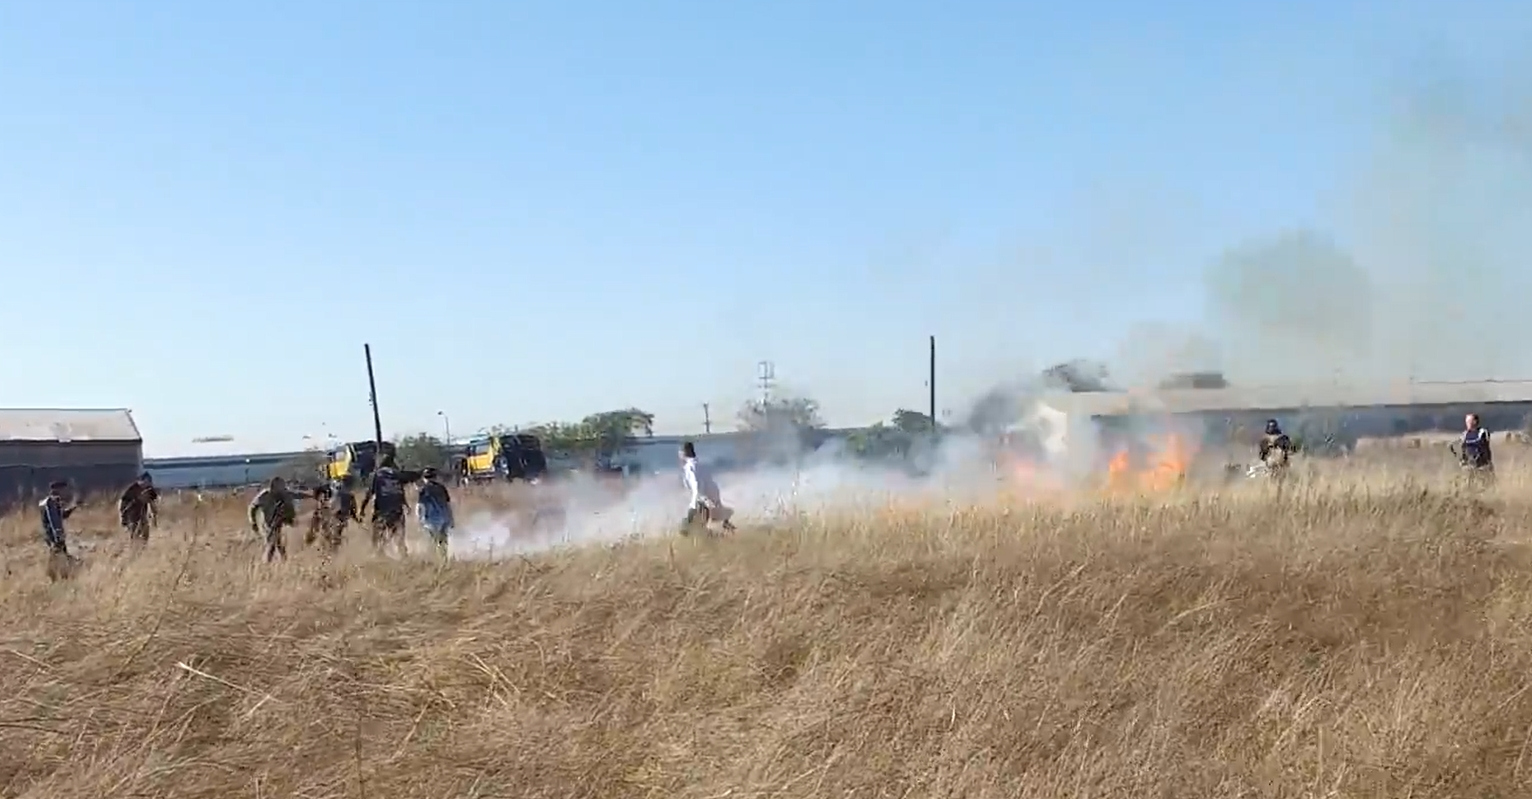
\includegraphics[width=0.6\linewidth]{images/fire_start} 

}

\caption{Beginning of a fire at Richmond Field Station, UC Berkeley}\label{fig:fire-start}
\end{figure}

\begin{figure}

{\centering 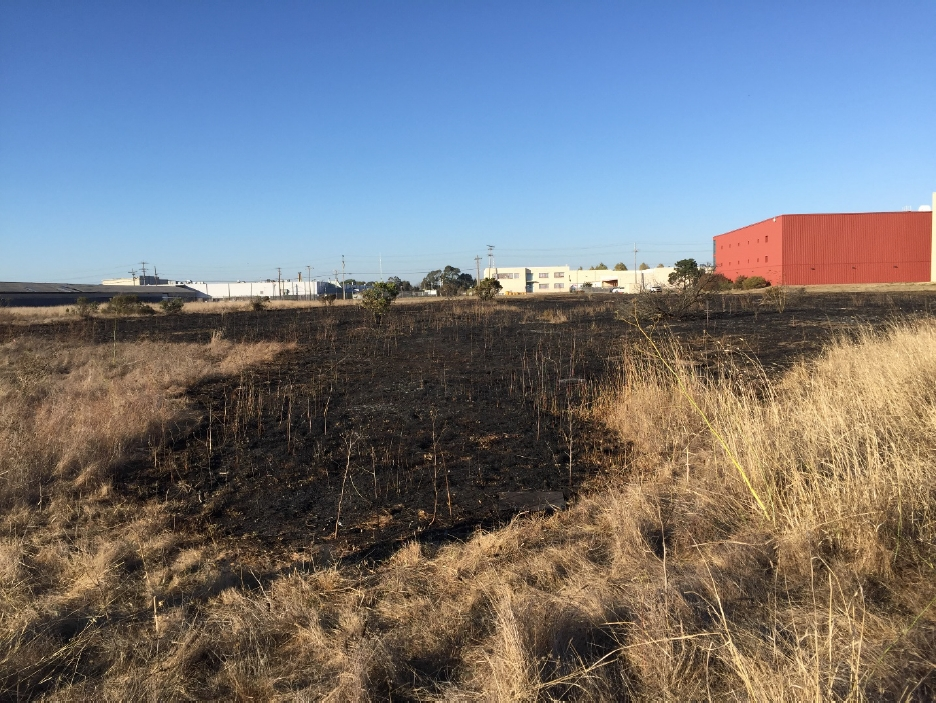
\includegraphics[width=0.6\linewidth]{images/fire_damage} 

}

\caption{Post fire damage from UAS accident at Richmond Field Station, UC Berkeley}\label{fig:fire-damage}
\end{figure}

The most common cause of UAS related fire is from misuse of \protect\hyperlink{LiPo}{LiPo} batteries. Special care should be taken when charging, discharging or storing \protect\hyperlink{LiPo}{LiPo} batteries. If the internal polymer cell of a \protect\hyperlink{LiPo}{LiPo} battery is exposed to air, a violent chemical reaction starts that could explode, but more commonly releases significant amounts of smoke and heat that can ignite other fire fuel sources. A \protect\hyperlink{LiPo}{LiPo} battery fire is typically caused by a physical puncture to the battery or from misuse, such as overcharging or electrical shorts.

In reviewing \protect\hyperlink{UASactivity}{UAS activity}, it is important that the \protect\hyperlink{RPIC}{RPIC} is aware of the relevant fire dangers and plans for fire safety. Consult the appropriate department (Fire, Field Safety, EH\&S) if there are concerns over fire risk. Minimize the potential for fire by monitoring where the UAS will be flying and ensure that if a fire was to occur, the \protect\hyperlink{RPIC}{RPIC} and any other persons, such as \protect\hyperlink{VO}{Visual Observers}, are prepared to respond appropriately.

Guidance for fire safety:

\begin{itemize}
\tightlist
\item
  Everyone should take a fire safety training course.
\item
  Avoid flying on high fire risk days.
\item
  Bring a fire extinguisher and a shovel/bucket of sand to field sites.
\item
  Ensure that a crew member has easy access to fire equipment.
\item
  Ensure that a crew member has easy access to reach any location where the \protect\hyperlink{UA}{Unmanned Aircraft} may crash.
\item
  Ensure that a crew member has the ability to report an emergency situation and can adequately provide directions for emergency personnel to reach the site.
\item
  When flying in high fire risk locations, use high quality, commercially available \protect\hyperlink{UA}{Unmanned Aircraft} with enclosed electronics.
\item
  Never fly a damaged or swollen battery.
\end{itemize}

\hypertarget{s-community-input}{%
\section{Community Input to Safety}\label{s-community-input}}

Another pathway that is recommended to improving UAS safety is to acknowledge the demand for \protect\hyperlink{UASactivity}{UAS activity} and engaging with the campus community to ensure there is a functional pathway to meet the demand. When the pathway is too restrictive, non-compliance increases and in turn decreases overall safety. Chapter \ref{ch-campus-groups} provides examples of campus UAS groups.

\hypertarget{ch-academic-use}{%
\chapter{Academic Use of UAS}\label{ch-academic-use}}

\hypertarget{uas-regulations-for-academic-use}{%
\section{UAS Regulations for Academic Use}\label{uas-regulations-for-academic-use}}

In Oct 2018, the FAA Reauthorization Act of 2018 was signed into law with two provisions significantly relevant for the University of California: Sec 349 - Exception for Limited Recreational Operations of Unmanned Aircraft and Sec 350 - Use of Unmanned Aircraft Systems at Institutions of Higher Education.

In Sec 350, Congress decreed that for the purposes of Sec 349, a recreational purpose shall include an unmanned aircraft system operated by and institution of higher education for educational or research purposes. The phrase `educational or research purposes' includes

\begin{itemize}
\tightlist
\item
  Instruction of students at the institution
\item
  Academic or research related uses of UAS that have been approved by the institution
\item
  Activities undertaken by the institution as part of research projects
\item
  Other academic activities approved by the institution
\end{itemize}

Given this wide definition, this provision is relevant to approximately 75\% of the University of California's UAS activity.

In Sec 349, Congress rewrote the statutes in the USC that was previously associated with `model aircraft' use, now referred to as `Recreational Operations.' To abide by the new `Recreational Operations' statute,
- The aircraft must be operated in accordance with or within the programming of a \protect\hyperlink{CBO}{Community-Based Organization} (CBO)
- The aircraft must be flown within \protect\hyperlink{VLOS}{VLOS}
- The aircraft must be operated in a manner that does not interfere with and gives way to any manned aircraft
- The operator must obtain prior approval from the FAA to operate within controlled airspace
- The aircraft may not fly more than 400 ft above ground level in uncontrolled airspace outside of designated `fixed-sites', and
- The operator must pass an aeronautical knowledge and safety test, and maintains proof of passage to be available to the FAA and law enforcement.

The new statutes can be interpreted as stricter than the previous `Model Aircraft' regulations, however, due to the inclusion of Sec 350, they offer a new and easier path forward for many University of California use. Previously, all research activity with UAS required a 14 CFR 107 Small Unmanned Aircraft System Remote Pilot Certificate (Drone License), which can be a challenging imposition in a 10 week quarter. The new regulations provide an alternative more suitable for introductory student UAS activity.

\begin{quote}
As of July 2019, the FAA has not finalized the implementation all aspects of Section 349. Currently, the aeronautical knowledge and safety exam has not been implemented. In the interim, the FAA is directing all `Recreational Operations' to abide by their interim rules as described here: \url{https://www.faa.gov/uas/recreational_fliers/}
\end{quote}

\begin{quote}
In the current interim rules, a UC student conducting academic activities may abide by the Recreational Operation regulations without a Drone License. Once the aeronautical knowledge and safety test has been established, all students wishing to abide by the Recreational Operation regulations must complete the test before flying.
\end{quote}

The application of the Policy still applies to the academic use of UAS, regardless of the regulations or statute that enables the \protect\hyperlink{UASactivity}{UAS activity}. All \protect\hyperlink{UASactivity}{UAS activity} subject to the Policy will require both a \protect\hyperlink{FR}{UAS Request Form} and a \protect\hyperlink{postflight}{UAS Post-Flight Report}, and be compliant with all applicable regulations. Depending on the specific \protect\hyperlink{UASactivity}{UAS activity}, the \protect\hyperlink{DLA}{Designated Local Authority} or \protect\hyperlink{LSP}{location specific policy or procedure} may additionally opt to issue open or standing approval under specific conditions that are deemed to be of low or minor risk on the condition of compliance with regulor submission of \protect\hyperlink{postflight}{Post-Flight Reports}.

\begin{figure}

{\centering 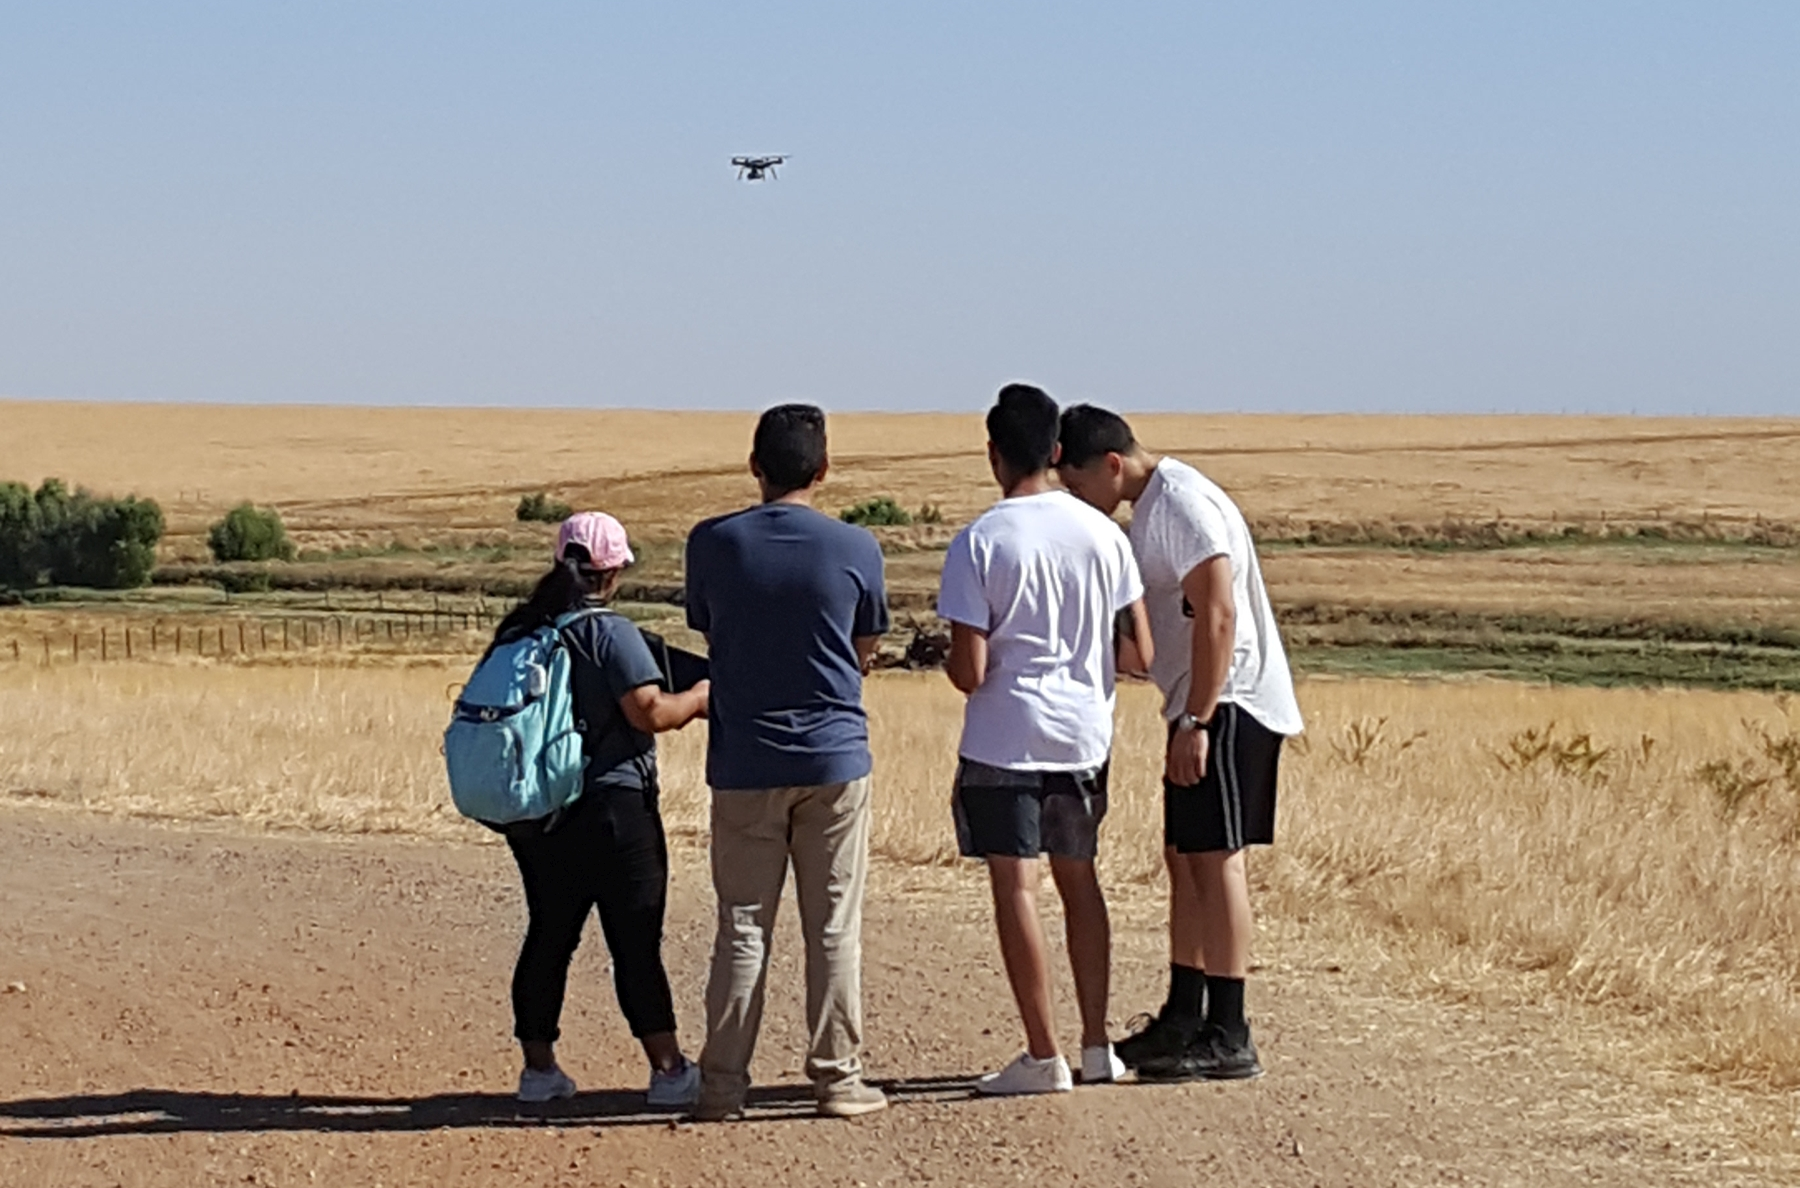
\includegraphics[width=0.7\linewidth]{images/students_flying} 

}

\caption{Students flying UC-owned UAS for coursework on a University Location}\label{fig:students-course}
\end{figure}

\hypertarget{frequently-asked-questions}{%
\section{Frequently Asked Questions}\label{frequently-asked-questions}}

\textbf{Which set of regulations do I fall under?}

For any academic related activity, it depends on whether your operations fit within the Recreational Operations exemption, otherwise you default to abiding by 14 CFR 107 regulations. Keep in mind that the Recreational Operations exemptions mandates compliance with a CBO's safety guidelines which may have stricter restrictions than 14 CFR 107. But if the purpose is for the University, but not academic (example: Media \& Communications, Facility Inspection), then you must abide by 14 CFR 107 regulations.

\textbf{When doing an academic activity, which set of regulations is better?}

There are advantages and disadvantages to both scenarios. In many cases, the new `Recreational Operations' may be the fastest path forward for simple, rural flight operations. At the current time, academic UAS activities that plan on flying in certain controlled airspace areas, over occupied structures, within 25 ft of another person, or outside of a reasonably controlled flying site, should proceed with 14 CFR 107 regulations.

\textbf{What are some of the airspace restrictions of `Recreational Operations'?}

Under `Recreational Operations,' \protect\hyperlink{RPIC}{RPICs} must obtain \protect\hyperlink{AA}{Airspace Authorization} similar to 14 CFR 107 operators either through (ref:LAANC) or (ref:DroneZone). However, unlike 14 CFR 107 operators, recreational RPICs are prohibited from requesting airspace altitudes that exceed the published altitude limit in the FAA's (ref:facility\_map). For example, at UC Santa Barbara, the Facility Map lists an allowable altitude of 0 ft AGL (effectively no flying) over the majority of campus. A licensed \protect\hyperlink{RPIC}{RPIC} operating under 14 CFR 107 may request and be granted special authorization to fly up to 100 ft AGL. However, an unlicensed \protect\hyperlink{RPIC}{RPIC} recreational operator would be prohibited from flying at all in the same location.

\textbf{What will the new Aeronautical Knowledge and Safety Test be like? How much will it cost?}

The FAA has not released details of the new test. However, it is anticipated that the test will be a shorter and simpler version of the 14 CFR 107 license exam, focusing on the bare minimum `rules of the road' and safety guidance. It is anticipated to take less than 1 hour for a novice, and would include embedded training, no prior studying necessary. No information regarding the cost has been announced, but is expected to be minimal, if any.

\textbf{What does the new regulations mean when it says `the programming of a Community-Based Organization'?}

The regulations do not require you to be a member of a \protect\hyperlink{CBO}{CBO} but that you abide by the rules and safety guidelines of a community-based organization. While not yet officially recognized, the \protect\hyperlink{AMA}{Academy of Model Aeronautics} is one of the largest CBOs and have an extensive safety history for those that abide by their rules and safety guidelines (located here: \url{https://www.modelaircraft.org/sites/default/files/100.pdf} ). These rules and safety guidelines often include prohibition on flying over people and buildings, limitations on suitable flying locations and specific standoff distances.

\textbf{What does the new regulations mean when it says ``The operator must obtain prior approval from the FAA to operate within controlled airspace''?}

The FAA is mandating that all controlled airspace access requests for recreational operations be routed through the Low Altitude Authorization Notification Capability system (LAANC) and not by calling the local airport tower. The LAANC system can provide instantaneous authorization via a 3rd party application such as Airmap, KittyHawk, or UASideKick for flight requests below a certain altitude depending on your location.

\textbf{I am planning to fly over a research site that is access controlled and the airspace is uncontrolled, do I need a Drone License?}

Typically not. This common scenario (such as in Figure \ref{fig:students-course}) will typically meet the necessary site requirements for Recreational Operations.

\textbf{I am planning to fly along the beach to monitor coastal erosion, do I need a Drone License?}

Unless the beach is to be closed to the public, this scenario will likely require a Drone License.

\textbf{I am planning on flying in the campus quad to test a flight controller, do I need a Drone License?}

If the airspace is uncontrolled (Class G), and the area within the campus quad is sufficiently cleared and closed to non-participants, then you do not need a Drone License. If you want to fly at UCI, UCSB or UCLA, then you will need to obtain an Airspce Authorization via LAANC.

\textbf{I do not have a Drone License, can I do a coursework assignment on the use of drones in building inspections?}

You may be able to do some flying without a drone license, however, you will not be allowed to fly over a building and must stay at least 25 ft from all non-participants, which may limit your ability to conduct effective analysis.

\textbf{I am a graduate student Teaching Asssistant and I would like to teach my students how to fly a drone? Do I need a license? Do the students need a license?}

If the site is sufficiently cleared and closed to non-participants, than everyone may have a chance to learn how to fly a drone without a drone license. However, additional safety precautions may be necessary.

\textbf{What is a fixed-site?}

A fixed-site is a location published by the FAA that recognizes that recreational activity may occur in that airspace. While the \protect\hyperlink{AMA}{Academy of Model Aeronautics} has obtained FAA recognition of fixed-sites, the FAA has not published information on the formation or requirements to have an area designated as one.

\hypertarget{personally-owned-uas-used-for-academic-research-or-coursework}{%
\section{Personally-owned UAS used for Academic Research or Coursework}\label{personally-owned-uas-used-for-academic-research-or-coursework}}

Some students, staff and faculty personally own UAS that they may wish to utilize for their respective activity.

Personally-owned UAS used for \protect\hyperlink{UB}{University Business} such as research or teaching are subject to the UC's UAS Policy, and as such a \protect\hyperlink{FR}{UAS Request Form} and a \protect\hyperlink{postflight}{UAS Post-Flight Report} must be completed. This use is allowed and may be provided free coverage under the UC's UAS liability insurance policy if it is properly documented and the \protect\hyperlink{UASactivity}{UAS activity} abides by the Policy. However, personally-owned UAS are not covered by the UC's Property Insurance policy - any damage to the UAS by theft, fire, in-transit or in-flight is not covered. Additionally, any UC-equipment attached to a personally-owned UAS is additionally not covered. It is strongly recommended that personal equipment is not used for \protect\hyperlink{UB}{University Business}

Personnally-owned UAS used for coursework, such as senior projects or homework assignments are not subject to the Policy unless operated on a \protect\hyperlink{UL}{University Location}. Additionally, they are not covered by either the UC's UAS liability insurance policy or the UC's Property Insurance policy. Students assume all risk and liability for their use.

\hypertarget{ch-common-considerations}{%
\chapter{Common UAS Policy Considerations}\label{ch-common-considerations}}

\hypertarget{indoor-use}{%
\section{Indoor Use}\label{indoor-use}}

The use of UAS of all sizes indoors is included within the scope of the Policy. Any UAS operated exclusively indoors is still considered legally a UAS, as an aircraft is defined as any contrivance invented, used, or designed to navigate, or fly in, the air\footnote{49 USC 40102}.

Though UAS that are operated exclusively indoors are exempt from FAA regulations, the Policy maintains oversight of indoor usage as their usage may still pose a safety risk, albeit easily mitigated.

Small UAS that weight less 0.55 lbs often pose little serious risk to persons, however, they may in rare situations cause property damage. One of the primary concerns of UAS of all sizes when operated indoors is damage to fire sprinklers. Mitigation may be accomplished by restricting usage to trained operators or by restricting usage within structures or implementing physical barriers to fragile items.

The \protect\hyperlink{DLA}{Designated Local Authority} or \protect\hyperlink{LSP}{location specific policy or procedure} may opt to issue specific restrictions or allowances on the use of UAS indoors. Specific flight information may not always be feasible, but should be reported when it is.

Example Statements for Indoor Use

\begin{itemize}
\tightlist
\item
  Student Clubs or classes must operate within a netted structure designed to prevent damage when operating indoors.
\item
  No flying within dorms.
\item
  Small UAS under 0.55 lbs may be operated indoors in a safe manner that minimizes risk to fire sprinklers.
\item
  A laboratory hazard assessment must be conducted prior to any indoor UAS usage.
\item
  Regular indoor \protect\hyperlink{UASactivity}{UAS activity} must submit estimated usage rates.
\end{itemize}

\hypertarget{recreational-uas-use}{%
\section{Recreational UAS Use}\label{recreational-uas-use}}

Recreational UAS, formerly known as `Model Aircraft' is a popular past-time since the dawn of modern aviation, and previously their use has largely been unregulated. However, in recent years, the regulatory landscape has undergone several changes that may be confusing. In 2012, Congress put into law the definition of Model Aircraft and the Special Rule for Model Aircraft in Public Law 112-95 (Section @ref\{ch-related-info\}). The Special Rule was codified in 14 CFR 101 with the publication of 14 CFR 107, but prevented the FAA from promulgating further regulations. This was repealed 6 years later in the FAA Reauthorization Act of 2018 which removed the legal distinction of `Model Aircraft,' and introduced new statutes within the United States Code under the authority of the FAA. As of this writing, the FAA has not yet promulgated regulations however, they are enforcing some of the new statutes.

In the current implementation, the \protect\hyperlink{RPIC}{RPIC} is exempt from 14 CFR 107 regulations (and \protect\hyperlink{RPC}{Remote Pilot Certificate} if the operator meets the required statutory conditions (See @ref() for details). In general, the UAS must be flown only for recreational purposes, must be flown with or within the programming of a \protect\hyperlink{CBO}{CBO}'s safety guidelines (such as the \protect\hyperlink{AMA}{Academy of Model Aeronautics}), must only be flown within \protect\hyperlink{VLOS}{VLOS}, must be flown in a manner that does not interfere with and gives way to any manned aircraft, must only be flown at altitudes less than 400 ft above the ground, and if in controlled airspace, the operator must obtain authorization. In most scenarios, recreational operations are more limited than licensed civil operations under 14 CFR 107.

Recreational UAS activity can be made safe and appropriate in large, open fields with limited opportunities for pedestrian intrusion. However, safety considerations arise when operating in small areas, or in the vicinity of people. It is important to note that under the \protect\hyperlink{AMA}{Academy of Model Aeronautics} safety code, recreational UAS must remain a minimum of 25 ft from all persons (or further depending on the context), with the exception of the \protect\hyperlink{RPIC}{RPIC}.

The use of recreational use of UAS is within the scope of the Policy to review. This enables the \protect\hyperlink{LSP}{location specific policy or procedure} or \protect\hyperlink{DLA}{Designated Local Authority} to issue restrictions or allowances on recreational UAS at a \protect\hyperlink{UL}{University Location}. This includes open or standing approvals in specific activities that are deemed to be of low or minor risk, when appropriate procedures are implemented and abided.

Some example recreational UAS policies or procedures statements that can be considered or utilized:

\begin{itemize}
\tightlist
\item
  A student club that wishes to hold a Recreational UAS club activity must submit safety documentation and reserve the appropriate space.
\item
  Recreational UAS activity is allowed at specific campus fields for any UC-affiliate who completes an online webinar that instructs on campus-specific policies and safety guidance.
\item
  Recreational UAS activity is prohibited within 100 ft of residential areas without prior approval.
\item
  Recreational UAS activity is prohibited during major campus events or ceremonies
\end{itemize}

It is recommended that the policies or procedures for recreational UAS include consultation with expected users and include student groups.

\hypertarget{non-university-business-use}{%
\section{Non-University Business Use}\label{non-university-business-use}}

All \protect\hyperlink{UASactivity}{UAS activity} on or within the property owned or managed by the UC must be approved before commencing. This includes when Non-University Business occurs at a \protect\hyperlink{UL}{University Location}.

Some common instances of Non-University Business Use

\begin{itemize}
\tightlist
\item
  \protect\hyperlink{rdparty}{3\textsuperscript{rd} Party} visitors to \protect\hyperlink{UL}{University Location}.
\item
  \protect\hyperlink{rdparty}{3\textsuperscript{rd} Party} hired by UC to perform a service.
\item
  A student or group of students providing a service.
\end{itemize}

The review process described in Chapter \ref{ch-review} remains the same. However, since they are not acting on behalf of the Regents of the University of California, they must obtain their own liability insurance and are responsible for obtaining any necessary authorization for regulatory compliance.

For departments or groups who may wish to use a UAS at a very infrequent rate, it may be more advisable to utilize an existing UC affiliated \protect\hyperlink{RPIC}{RPIC} rather than hiring a \protect\hyperlink{rdparty}{3\textsuperscript{rd} Party} operators.

A common scenario is found at a \protect\hyperlink{UL}{University Location} in controlled airspace (Non-Class G airspace). The \protect\hyperlink{SDA}{Systemwide Designated UAS Authority} has obtained \protect\hyperlink{AA}{Airspace Authorizations} for many such locations, however it is not transferable to non-University Business Use. For example, if a researcher hires a \protect\hyperlink{RPIC}{RPIC} for \protect\hyperlink{UASactivity}{UAS activity} at a research site within a military controlled airspace, the \protect\hyperlink{rdparty}{3\textsuperscript{rd} Party} \protect\hyperlink{RPIC}{RPIC} must obtain their own \protect\hyperlink{AA}{Airspace Authorization}. This also applies to students who perform a commercial service at a \protect\hyperlink{UL}{University Location}. Even though the student is a UC student, the student's purpose is not \protect\hyperlink{UB}{University Business} and thus falls into Non-University Business Use.

Compliance with FAA regulations have improved since the enactment of 14 CFR 107 regulations, however, be mindful that hired \protect\hyperlink{rdparty}{3\textsuperscript{rd} Party} operators are often unfamiliar with the cadence and activity of a university campus, especially around classrooms and residential dorms. The \protect\hyperlink{DLA}{Designated Local Authority} is often in the best position to advise \protect\hyperlink{rdparty}{3\textsuperscript{rd} Party} operators when areas may be safe or unsafe.

Liability insurance is another common issue for \protect\hyperlink{rdparty}{3\textsuperscript{rd} Party} operators. It is important to note that Aviation/UAS liability insurance is not a common rider for general or commercial liability policies, and without it, the insurance company will not pay out for any damages caused by a UAS. In most situations, Aviation/UAS liability insurance coverage must be purchased seperately. It is important for the Campus Risk Manager to vet or evaluate whether the \protect\hyperlink{rdparty}{3\textsuperscript{rd} Party} has the appropriate coverage.

\hypertarget{emergency-or-first-responder-use-of-uas}{%
\section{Emergency or First Responder Use of UAS}\label{emergency-or-first-responder-use-of-uas}}

The Policy states that the operation of UAS by emergency first responders may be exempt from the policy based on determination of emergency needs. First responders should refer to their internal department protocols. However, the \protect\hyperlink{SDA}{Systemwide Designated UAS Authority} is available to assist in the development of first responder protocols for UAS usage.

The use of UAS is on the rise nation-wide as their potential for saving lives are realized - providing aerial views for search \& rescue, monitoring for mudslides or other hazardous situations. First responders may operate under as a \protect\hyperlink{PAO}{PAO} (if a public agency, such as law enforcement) or under 14 CFR 107. All rules and regulations are applicable. Additional regulatory flexibility is provided through the \protect\hyperlink{FAA}{FAA}'s Special Governmental Interest (SGI) process (FAA Order JO 7200.23A).

\hypertarget{special-governmental-interest-process}{%
\subsection{Special Governmental Interest Process}\label{special-governmental-interest-process}}

Through its SGI process, the FAA may expedite the issuance to qualifying UAS operations of 1) addendums to pre-existing {[}COAs{]} or 2) \protect\hyperlink{AA}{Airspace Authorizations} and \protect\hyperlink{AW}{Airspace Waivers} to 14 CFR 107 operators.

The FAA may rapidly approve through its SGI process \protect\hyperlink{COA}{COA} addendums and 14 CFR 107 authorizations and waivers UAS operations that:

\begin{itemize}
\tightlist
\item
  Fly in airspace (including controlled airspace and disaster \protect\hyperlink{TFR}{TFRs}) and/or at altitudes not otherwise permitted.
\item
  Fly \protect\hyperlink{BVLOS}{BVLOS}.
\item
  Fly at night.
\end{itemize}

Obtaining approval through the SGI process

\begin{enumerate}
\def\labelenumi{\arabic{enumi}.}
\tightlist
\item
  You must already be an existing 14 CFR 107 \protect\hyperlink{RPIC}{RPIC} with a current certificate OR you must have an existing \protect\hyperlink{COA}{COA}. The \protect\hyperlink{FAA}{FAA} will not grant emergency approval for casual or recreational drone pilots.
\item
  Fill out the \href{https://www.faa.gov/uas/getting_started/emergency_approval/media/UAS-SGI_waiver_approval_request_form.docx}{Emergency Operation Request Form (MS Word)} and send to the FAA's System Operations Support Center (SOSC) at \href{mailto:9-ator-hq-sosc@faa.gov}{\nolinkurl{9-ator-hq-sosc@faa.gov}}.
\item
  If the proposed UAS flight is to be conducted within a disaster \protect\hyperlink{TFR}{TFR}, the \protect\hyperlink{FAA}{FAA}'s SOSC, as appropriate, may need to pre-coordinate the requested operation with a responsible Incident Commander or Unified Command (IC/UC) to ensure their activity will support or, at a minimum, not interfere with broader response and recover efforts.
\end{enumerate}

The \protect\hyperlink{FAA}{FAA} will then coordinate with the effected Air Traffic facilities to:

\begin{enumerate}
\def\labelenumi{\arabic{enumi}.}
\tightlist
\item
  Review your proposed operation and determine whether it meets the necessary criteria for emergency approval.
\item
  Implement any necessary mitigations to minimize impact on other air traffic operations.
\item
  Contact you within one hour or sooner regarding the status of your request or to request additional information.
\end{enumerate}

\textbf{If approved,} the \protect\hyperlink{FAA}{FAA} will add an amendment to your existing \protect\hyperlink{COA}{COA} or Remote Pilot Certificate that authorizes you to fly under certain conditions for the specified operation.

\textbf{If denied,} operators should NOT fly outside the provisions of their existing \protect\hyperlink{COA}{COA} or 14 CFR 107. Operators have the option to amend their requests.

\hypertarget{international-students-visiting-scholars-and-undocumented-students}{%
\section{International Students, Visiting Scholars and Undocumented Students}\label{international-students-visiting-scholars-and-undocumented-students}}

The UC attracts students, staff and faculty from all around the world. This unfortunately can complicate the already complex UAS regulatory environment. There are two issues: 1) obtaining a 14 CFR 107 Remote Pilot Certificate and 2) operating under 14 CFR 107. It is possible for it to be legal for a foreign national to obtain a 14 CFR 107 Remote Pilot Certificate but not be eligible to use it for a specific purpose.

\hypertarget{eligibility-for-a-14-cfr-107-remote-pilot-certificate}{%
\subsection{Eligibility for a 14 CFR 107 Remote Pilot Certificate}\label{eligibility-for-a-14-cfr-107-remote-pilot-certificate}}

The Remote Pilot Certificate does not require U.S. citizenship.

Requirements

\begin{itemize}
\tightlist
\item
  Be at least 16 years of age
\item
  Be able to read, speak and understand the English language. If the applicant is unable to meet one of these requirements due to medical reasons, the \protect\hyperlink{FAA}{FAA} may place such operation limitations on that applicant's certificate as are necessary for the safe operation of the small unmanned aircraft.
\item
  Not know or have reason to know that he or she has a physical or mental condition that would interfere with the safe operation of a small unmanned aircraft system.
\end{itemize}

However, to take the \protect\hyperlink{FAA}{FAA} Airman Knowledge Exam, the proponent must prove their identity with a valid photo ID that includes their date of birth, signature and physical, residential address.

For U.S. Citizens and U.S. Resident Aliens, this may be accomplished with one of the following:

\begin{itemize}
\tightlist
\item
  Driver Permit or License issued by a U.S. state or territory
\item
  U.S. Government Identification Card
\item
  U.S. Military Identification Card
\item
  Passport
\item
  Alien Residency Card
\end{itemize}

For Non-U.S. Citizens, this may be accomplished with one of the following:

\begin{itemize}
\tightlist
\item
  Passport and a Driver permit or license issued by a U.S. state or territory.
\item
  Passport and an Identification card issued by any governmental entity.
\end{itemize}

\hypertarget{foreign-nationals-operating-an-suas}{%
\subsection{Foreign Nationals operating an sUAS}\label{foreign-nationals-operating-an-suas}}

While a foreign national is permitted to obtain a Remote Pilot Certificate, there are additional federal regulations that apply, and in some cases, certain activity requires additional permitting or may be prohibited completely. Under federal law, an aircraft operated by a foreign national in civil airspace is generally considered a foreign registered aircraft and is subject to regulations found in \href{https://www.faa.gov/uas/resources/foreign_operators/}{14 CFR 375}.

It is important to note that this restriction applies only for UAS and sUAS for non-recreational activity. Any use under recreational operations, such as individual recreation, club recreation or approved academic activity, is not subject to 14 CFR 375 restrictions.

How this applies:

\begin{itemize}
\tightlist
\item
  An international student with a Remote Pilot Certificate may operate a UC-owned sUAS for specific \protect\hyperlink{UB}{University Business}.
\item
  An international student with a Remote Pilot Certificate may not operate a personally-owned sUAS for \protect\hyperlink{UB}{University Business} or for other non-recreational activity without at 14 CFR 375 permit.
\item
  An international student may conduct recreational UAS activity for personal recreation
\item
  An international student may conduct recreational UAS activity for a classroom homework assignment, senior project, or approved academic activity, including research.
\end{itemize}

\#\#\#Undocumented Students
The University of California is home to many undocumented students, including those enrolled in Deferred Action for Childhood Arrivals (DACA). The University of California is steadfast in ensuring the education of all students admitted into the UC regardless of their immigration status\footnote{\url{https://universityofcalifornia.edu/press-room/uc-president-napolitano-statement-decision-end-daca-program}}. This section addresses the UAS restrictions and opportunities for undocumented students.

Unfortunately, since the Remote Pilot Certificate is a federal certificate, it requires a federally recognized identification. Statewide initiatives such as AB60 Driver's Licenses are not valid as identification for the FAA Airman Knowledge Exam.

Students with a DACA identification card are eligible to take the FAA Airman Knowledge Exam. For the purposes of Part 107, they are not considered foreign nationals and may operate under Part 107.

It is important to note that there are three alternative solutions for undocumented students to utilize UAS in their education.

\begin{itemize}
\tightlist
\item
  Undocumented students are not restricted to operate recreational UAS operations. This applies to the use of UAS for individual recreation, club recreation or for approved academic activities such as coursework, senior projects or academic research.
\item
  Undocumented students are not restricted to operate UAS in indoor facilities, such as outdoor drone cages or inside UC buildings. Undocumented students may engage in UAS related research in any location where \protect\hyperlink{FAA}{FAA} regulations are not applicable.
\item
  For outdoor usage, if a licensed UAS operation is necessary, undocumented students may be in control of a UAS if and only if the student is under the direct supervision of a licensed \protect\hyperlink{RPIC}{RPIC} and the \protect\hyperlink{RPIC}{RPIC} has the ability to immediately take direct control of the flight of the sUAS.
\end{itemize}

\hypertarget{ch-services}{%
\chapter{Services Available}\label{ch-services}}

\hypertarget{sec-UCDrones}{%
\section{UC Drones Web Application}\label{sec-UCDrones}}

UC Risk and Safety Solutions launched an organizational tool called \protect\hyperlink{UCDrones}{UC Drones} to help track UC-owned \protect\hyperlink{UA}{Unmanned Aircraft}, review and approve \protect\hyperlink{UASactivity}{UAS activity} (Figure \ref{fig:UCDrones}. It can be found at \url{http://ehs.ucop.edu} as part of the UC Risk and Safety suite of web applications.

\begin{figure}

{\centering 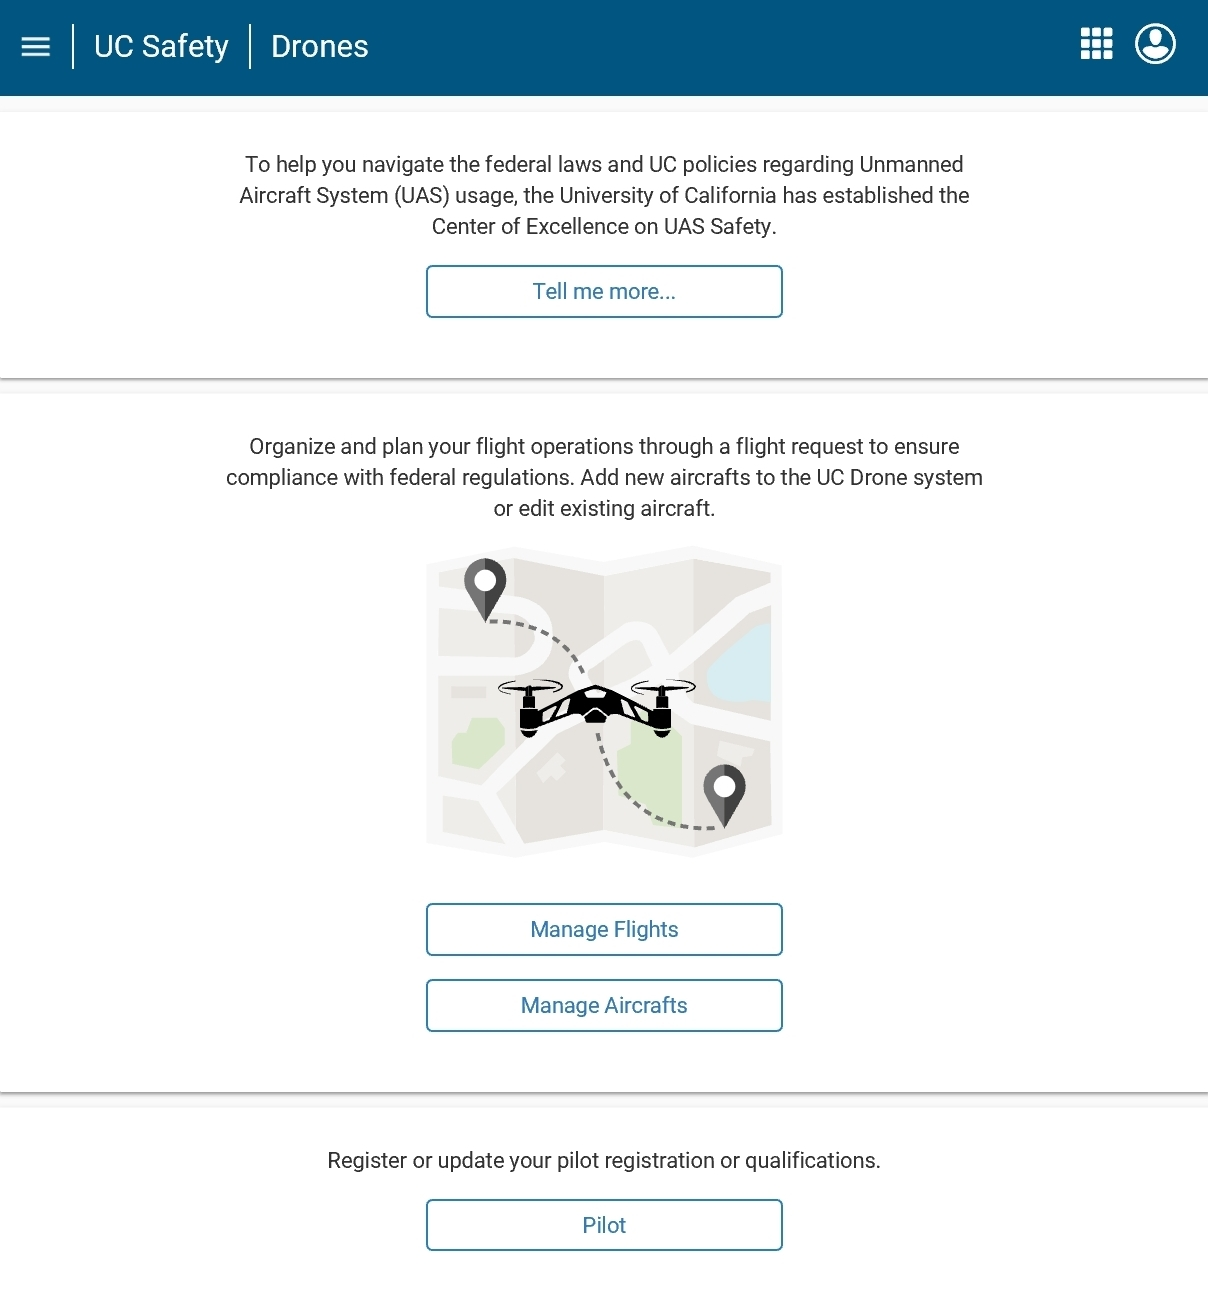
\includegraphics[width=0.6\linewidth]{images/UCDrones} 

}

\caption{UC Drones}\label{fig:UCDrones}
\end{figure}

The use of \protect\hyperlink{UCDrones}{UC Drones} is encouraged, but not mandatory. A \protect\hyperlink{UL}{University Location} may opt to utilize \protect\hyperlink{UCDrones}{UC Drones} or develop their own solution for the management of UAS records, flight authorizations and flight records.

A \protect\hyperlink{DLA}{Designated Local Authority} may utilize \protect\hyperlink{UCDrones}{UC Drones} as means to funnel UAS operation requests, provide notification, grant authorization and document flight activities. \protect\hyperlink{UCDrones}{UC Drones} is expected to continue to release additional features as requested. Future enhancement include automated risk assessments and approvals for low-risk activity, real-time weather and airspace assessments and integration with \protect\hyperlink{FAA}{FAA} systems.

\hypertarget{sec-FAA-filing}{%
\section{Filing of FAA Authorizations}\label{sec-FAA-filing}}

The \protect\hyperlink{SDA}{Systemwide Designated UAS Authority} is available to assist in the filing of \protect\hyperlink{FAA}{FAA} required authorizations. This includes

\begin{itemize}
\tightlist
\item
  \protect\hyperlink{AA}{Airspace Authorization} for \protect\hyperlink{UASactivity}{UAS activity} in controlled airspace
\item
  \protect\hyperlink{AW}{Airspace Waiver} for \protect\hyperlink{UASactivity}{UAS activity} not allowed with an \protect\hyperlink{AA}{Airspace Authorization}
\item
  Waiver under 14 CFR 107.200. Commonly includes authorizations for night-time operations, flight altitudes above 400 ft \protect\hyperlink{AGL}{AGL} or multiple aircraft.
\item
  \protect\hyperlink{PAO}{PAO} \protect\hyperlink{COA}{COA} for \protect\hyperlink{UASactivity}{UAS activity} that meets the criteria of a \protect\hyperlink{PAO}{PAO}
\item
  Registering of \protect\hyperlink{UA}{Unmanned Aircraft} used in foreign nations that require 14 CFR 47 registration.
\end{itemize}

\hypertarget{sec-training}{%
\section{UAS Training and Certification}\label{sec-training}}

The \protect\hyperlink{SDA}{Systemwide Designated UAS Authority} supports the development of local UAS training programs and support programs. Material may be provided upon request. In addition, the \protect\hyperlink{SDA}{Systemwide Designated UAS Authority} is developing specialized training and certification programs for uncommon scenarios.

\textbf{Current Training Modules Available}

\begin{itemize}
\tightlist
\item
  UC Night-flying Training
\item
  Flight Operations over People
\item
  Visual Observer
\item
  Advanced UAS Training
\end{itemize}

\hypertarget{ch-campus-groups}{%
\chapter{Campus Drone Groups}\label{ch-campus-groups}}

As campuses grow into their UAS usage, it may be advisable to develop and institute `drone' groups. Community involvement is an effective means to disseminate knowledge and establish a safety program. Below are some examples of groups - there are no requirements or restrictions for the formation of any of these groups or of any of the example tasks.

\hypertarget{uas-campus-policy-or-procedure-group}{%
\section{UAS Campus Policy or Procedure Group}\label{uas-campus-policy-or-procedure-group}}

The Policy allows for a \protect\hyperlink{UL}{University Location} to appoint a \protect\hyperlink{DLA}{Designated Local Authority}. As a \protect\hyperlink{UL}{University Location} may see fit and in accordance to their \protect\hyperlink{UL}{University Location} policy, the \protect\hyperlink{UL}{University Location} may organize a working group or committee to develop \protect\hyperlink{UL}{University Location} specific policy or procedures. See Chapter \ref{ch-campus-auth} for further information regarding \protect\hyperlink{UL}{University Location} jurisdiction and authority.

Example Tasks

\begin{itemize}
\tightlist
\item
  Develop or advise \protect\hyperlink{LSP}{location specific policy or procedure}.
\item
  Review efficiency and compliance of campus \protect\hyperlink{UASactivity}{UAS activity}.
\item
  Review high risk or other significant unique \protect\hyperlink{UASactivity}{UAS activity}.
\item
  Develop streamlined procedures for low-risk \protect\hyperlink{UASactivity}{UAS activity}.
\item
  Standards regarding privacy.
\end{itemize}

\hypertarget{uas-campus-safety-group}{%
\section{UAS Campus Safety Group}\label{uas-campus-safety-group}}

Another valuable group is a \protect\hyperlink{UL}{University Location} is a safety group. In contrast to a Policy or Procedure group, a safety group would provide safety training and assist in \protect\hyperlink{UASactivity}{UAS activity} development and planning.

Example Tasks

\begin{itemize}
\tightlist
\item
  Provide UAS training to the campus.
\item
  Develop Standard Operating Procedures for common \protect\hyperlink{UASactivity}{UAS activity}.
\item
  Promote UAS safety to the campus.
\item
  Identify and manage safe locations for \protect\hyperlink{UASactivity}{UAS activity}.
\end{itemize}

\hypertarget{uas-campus-service-or-advocacy-group}{%
\section{UAS Campus Service or Advocacy Group}\label{uas-campus-service-or-advocacy-group}}

Many UC students and researchers have significant experience in the use and operation of UAS. It would be advantageous to leverage this this knowledge and experience by providing opportunities for UAS users to interact on a regular basis with the campus. This may come in the form of a service center or other advocacy group.

Example Tasks

\begin{itemize}
\tightlist
\item
  Provide \protect\hyperlink{UASactivity}{UAS activity} as a service.
\item
  Encourage innovative \protect\hyperlink{UASactivity}{UAS activity}.
\item
  Organize or support \protect\hyperlink{UASactivity}{UAS activity} by student clubs.
\item
  Hold UAS-related events to provide networking and community building.
\end{itemize}

\hypertarget{ch-enforcement}{%
\chapter{Enforcement or Restrictions for UAS}\label{ch-enforcement}}

The growth of UAS on our UC campuses has also led to rising concerns over inappropriate UAS usage. This Chapter provides guidance on the enforcement of the Policy and campus responses.

\hypertarget{enforcement-and-safety}{%
\section{Enforcement and Safety}\label{enforcement-and-safety}}

It is important to note that while the Policy seeks to improve UAS safety by providing oversight, overuse of UAS restrictions may be counter productive.

In conjunction with positive means for advocating for UAS safety, there is a role for enforcement of the Policy. The decision to approve or deny \protect\hyperlink{UASactivity}{UAS activity} should not be taken lightly. The best outcome for a complicated scenario should be a discussion of safety concerns and mitigration strategies. However, there will be cases when a formal denial declaration is necessary and a template is provided in Chapter \ref{ch-example-denial}.

\hypertarget{appropriate-reasons-to-restrict-uas-usage}{%
\section{Appropriate Reasons to Restrict UAS usage}\label{appropriate-reasons-to-restrict-uas-usage}}

While the Policy states that the \protect\hyperlink{UASactivity}{UAS activity} must be reviewed for specific compliance issues, a \protect\hyperlink{DLA}{Designated Local Authority} may also review for impacts to \protect\hyperlink{UB}{University Business} and other local issues. Ultimately, there may be additional reasons to restrict UAS usage unrelated to legal compliance. Below are some recommendations for a non-exclusive list of appropriate reasons to restrict UAS usage as well as some reasons that may be overly cautious.

\textbf{Appropriate Reasons}

\begin{itemize}
\tightlist
\item
  Proximity to Medical Helipads
\item
  Privacy concerns within 100 ft distance
\item
  Expected heavy pedestrian or vehicular traffic at the date/time of \protect\hyperlink{UASactivity}{UAS activity}
\item
  Impacts to wildlife
\item
  Detrimental to University Business
\item
  Lack of planning or safety mitigations
\end{itemize}

\textbf{Overly Cautious Reasons}

\begin{itemize}
\tightlist
\item
  Privacy concerns at distances greater than 100 ft
\item
  Noise concerns at distances greater than 200 ft
\item
  Pedestrian safety when campus activity is non-existent
\item
  Requiring advanced training in low risk locations
\item
  Risk of damage to outdoor sports equipment or facilities with UAS under 4.4 lbs
\end{itemize}

\hypertarget{unauthorized-use-of-uas-on-a-university-location}{%
\section{Unauthorized use of UAS on a University Location}\label{unauthorized-use-of-uas-on-a-university-location}}

Depending on the situation, there are several different approaches. The primary response should be education rather than punishment. Below are four example situations and an appropriate response.

\begin{itemize}
\tightlist
\item
  If there's an immediate and evident safety threat (maliciously endangering others, reckless behavior, etc), call local law enforcement.
\item
  If the operation of a drone is impeding \protect\hyperlink{UB}{University Business} such as disrupting an event or preventing authorized \protect\hyperlink{UASactivity}{UAS activity}, ask the person to stop and to leave. If they refuse, then it may be considered trespass and contact local law enforcement.
\item
  If no one is at immediate risk, the \protect\hyperlink{UASactivity}{UAS activity} is not impeding \protect\hyperlink{UB}{University Business}, but the \protect\hyperlink{UASactivity}{UAS activity} is likely a violation of an applicable federal, state or local regulation, ask the operator to stop and point out the violation. If the operator persists, collect information, and report to the \protect\hyperlink{SDA}{Systemwide Designated UAS Authority}.
\item
  If the only violation is that the \protect\hyperlink{UASactivity}{UAS activity} was not requested or approved (everything is legal, safe and its not interrupting anything), ask them to stop, inform them of the policy, and the reason of the policy. Law enforcement action is not advisable, however, the situation may be documented and administrative action may be taken, if appropriate.
\end{itemize}

\hypertarget{common-arguments-and-potential-counters}{%
\section{Common Arguments and Potential Counters}\label{common-arguments-and-potential-counters}}

Occasionally a UAS operator may disagree with the review or potential enforcement action. In many cases, the disagreement may stem from a misunderstanding of regulations or miscommunication of policy. The following lists some common arguments and a response to clarify the underlying misunderstanding.

\textbf{Argument: Only the \protect\hyperlink{FAA}{FAA} may create airspace regulations}

The campus is not creating airspace regulations. It has a policy on where a person may or may not operate a UAS, model aircraft or drone. While on campus property, a person may not operate a UAS without prior approval. The \protect\hyperlink{FAA}{FAA} claims sole jurisdiction of the airspace and overflight\footnote{49 U.S.C. 40103(b)}, but laws and policies such as land-use, zone, privacy and trespass are not subject to Federal Regulation\footnote{pg. 42194, Federal Register, Vol. 81, No 124}.

\textbf{Argument: This area is open to the public, why can't I fly my drone here?}

While the University of California is a public agency, this does not mean that its property is not managed. The University has a responsibility to ensure the safety and security of everyone\footnote{UCOP Policy PACAOS-40.00 Policy on Use of University Properties}. In order to manage the property, the campus has established that a person may not operate a UAS without prior approval.

\textbf{Argument: I'm operating as a hobbyist, there are no regulations}

Hobbyist operators are subject to Exception for Recreational UAS statutes introduced by the FAA Reauthorization Act of 2018. In addition, UAS regulations do not supersede land-use, trespass or privacy regulations. The campus has put into policy that while on campus property, a person may not operate a UAS or drone without prior approval.

\textbf{Argument: This is a toy, not a Drone}

Congress has defined \protect\hyperlink{UA}{Unmanned Aircraft} as any aircraft that is operated without the possibility of direct human intervention from within or on the aircraft. This definition has no size or weight limit. While the operator may be using the \protect\hyperlink{UA}{Unmanned Aircraft} as a toy, it however is regulated as above. Even though Unmanned Aircraft under 0.55 lbs do not require registration, they are not exempt from regulation.

\textbf{Argument: I have legal authorization from the FAA to fly here}

A licensed sUAS operator may have permission to use the airspace, but the campus still has jurisdiction to create policy on where a person may or may not operate a drone on campus property. The \protect\hyperlink{FAA}{FAA} makes it clear that an \protect\hyperlink{AA}{Airspace Authorization} or \protect\hyperlink{AW}{Airspace Waiver} does not grant physical property access rights. Under `Standard Provisions' of an \protect\hyperlink{AA}{Airspace Authorization} or \protect\hyperlink{AW}{Airspace Waiver}, there is a line that states `Note - This certificate constitutes a waiver of those Federal Rules or regulations specifically referred to above. It does not constitute a waiver of any State law or local ordinance.'

\textbf{Argument: I'm not causing any problems}

The campus has the jurisdiction to determine what is appropriate use of its facilities\footnote{UCOP Policy PACAOS-40.00 Policy on Use of University Properties}. If a person is causing legitimate concerns on campus safety, campus security, privacy or interfering with \protect\hyperlink{UB}{University Business}, that person is not using campus facilities appropriately.

\hypertarget{ch-privacy}{%
\chapter{Best Practices for UAS Privacy}\label{ch-privacy}}

In the United States today, the use of UAS for both recreation and commercial use are becoming ever more prominent. UAS may be used for a variety of applications, including photography and videography. The capture and use of photographs and videos from a UAS platform raises new concerns on the rights, privacies, and permissions that involve both the operators of UAS and individuals that are uninvolved in the operation. The University of California recognizes the important value of privacy and strives to achieve an appropriate balance ensuring an appropriate level of privacy, nurturing an environment of openness, honoring its obligation as a public institution to remain transparent while safe guarding information about individuals.

\textbf{Best Practices}

\begin{itemize}
\tightlist
\item
  \textbf{Do Not} use a UAS to monitor or record activities where there is a reasonable expectation of privacy.
\item
  \textbf{Do Not} use a UAS for unapproved recordings of any campus events or performances, or for any unlawful purposes.
\item
  \textbf{Do Not} fly a UAS over private property without prior approval.
\item
  \textbf{Do Not} use a UAS to harass people or intentionally disrupt events
\item
  \textbf{Do Not} use a UAS for the specific purpose of persistent and continuous collection of identifiable data about individuals without the consent of the data subjects.
\item
  \textbf{Do Not} retain identifiable data longer than reasonably necessary to fulfill a purpose.
\item
  \textbf{Do Not} knowingly publicly disclose data collected with a UAS without undertaking a reasonable effort to obfuscate or de-identify identifiable data unless the data subjects provide specific consent to the disclosure.
\item
  \textbf{Do} make a reasonable effort to provide prior notice to individuals of the general timeframe and area that they may anticipate a UAS intentionally collecting data.
\item
  \textbf{Do} establish and make available a Privacy Policy for UAS data if the UAS may intentionally or unintentionally collected identifiable data. The policy should be appropriate to the size and complexity of the data collected.
\item
  \textbf{Do} be considerate of other people's concerns over privacy, security and safety.
\item
  \textbf{Do} contact the Office of Research Compliance and Integrity if identifiable data is to be used for human-subject research.
\item
  \textbf{Do} take steps to ensure the security of any identifiable data.
\end{itemize}

\hypertarget{ch-FAQs}{%
\chapter{Frequently Asked Questions}\label{ch-FAQs}}

This is a list of Frequently Asked Questions related to the Policy and its implementation.

\begin{quote}
A short list of Frequently Asked Questions for end-users can be found at: \url{https://www.ucop.edu/safety-and-loss-prevention/environmental/program-resources/unmanned-aircraft-systems-safety.html}
\end{quote}

\hypertarget{scope-of-the-policy}{%
\section{Scope of the Policy}\label{scope-of-the-policy}}

\begin{itemize}
\item
  \textbf{Why is oversight necessary?}

  There are many arguments for the UC to mandate oversight; not all of them may be applicable for every situation but collectively form sufficient justification. The UC has an obligation to be fully compliant with all applicable regulations. In some cases, there are specific regulatory compliance obligations to meet. In other cases, the UC's UAS insurance has compliance obligations. There are many concerns over the usage of UAS on-campus from a public safety and privacy perspective. In other cases, there are arguments that UC business use should be able to take priority over \protect\hyperlink{rdparty}{3\textsuperscript{rd} Party} use. None of these determinations can be made unless there is a mechanism to screen for issues. It must be noted that the Policy does not prohibit procedures to ensure an alternative means of compliance.
\item
  \textbf{The \protect\hyperlink{FAA}{FAA} has already created UAS regulations. Why is the Policy necessary?}

  The \protect\hyperlink{FAA}{FAA} has sole jurisdiction of the airspace and overflight, however this is also the extent of their jurisdiction. The \protect\hyperlink{FAA}{FAA} regulations do not address other regulatory compliance issues such as export control, privacy, trespass harassment of wildlife or other land-use issues. The \protect\hyperlink{FAA}{FAA} regulations also do not address the prioritization of \protect\hyperlink{UB}{University Business} or other campus policies on commercial use or filming. In addition, \protect\hyperlink{FAA}{FAA} regulations regarding UAS are in flux and may change with acts of Congress, court cases and through traditional rule making processes. Incorrect interpretations of UAS regulations is common. The Policy enables oversight to ensure compliance while regulations are in flux.
\item
  \textbf{Does this policy apply to balloons and/or rockets?}

  The policy does not apply to balloons or rockets.
\item
  \textbf{Does the policy apply to international \protect\hyperlink{UASactivity}{UAS activity}?}

  Yes, the policy applies to international \protect\hyperlink{UASactivity}{UAS activity}. The policy requires that \protect\hyperlink{UASactivity}{UAS activity} must comply with all applicable regulations; in the case of international locations, the applicable regulations would be the local regulations of the international site. To the extent that safety practices or best practices may differ internationally, the \protect\hyperlink{UASactivity}{UAS activity} should be reviewed on a case-by-case basis.
\item
  \textbf{Is possession of a Remote Pilot Certificate sufficient for approval for \protect\hyperlink{UASactivity}{UAS activity}?}

  The Remote Pilot Certificate is an indication that the \protect\hyperlink{RPIC}{RPIC} passed a knowledge exam. It does not attest to the quality of the \protect\hyperlink{RPIC}{RPIC}'s experience with flying UAS or the \protect\hyperlink{RPIC}{RPIC}'s knowledge of safety practices. By itself, the Remote Pilot Certificate is not sufficient in all cases. However, where \protect\hyperlink{UASactivity}{UAS activity} risk is mitigated through other means such as remote location, or while operating a low risk \protect\hyperlink{UA}{Unmanned Aircraft}, simply having earned the \protect\hyperlink{RPC}{Remote Pilot Certificate} may be sufficient.
\item
  \textbf{What would happen if there's a disagreement between the \protect\hyperlink{DLA}{Designated Local Authority} and the \protect\hyperlink{SDA}{Systemwide Designated UAS Authority}?}

  In most cases, if a \protect\hyperlink{DLA}{Designated Local Authority} is appointed, the \protect\hyperlink{DLA}{Designated Local Authority} would adjudicate the final ruling. If there is a question over regulatory compliance, the \protect\hyperlink{SDA}{Systemwide Designated UAS Authority} and General Counsel would adjudicate clarification over the regulatory compliance aspect.
\item
  \textbf{What are the consequences of failing to abide by policy?}

  Existing policies address non-compliance. On how enforcement action is to be handled (as directed at a system level) for policy violations, please refer to PACAOS 100.00 for students, PPSM 62-65 for staff, APM 015-016 for faculty, and APM 140,150 for non-senate academic appointees.
\end{itemize}

\hypertarget{requesting-a-uas-flight}{%
\section{Requesting a UAS Flight}\label{requesting-a-uas-flight}}

\begin{itemize}
\item
  \textbf{What information is required for a Flight Request?}

  The policy states that the request must provide sufficient information to complete the review requirements on `Compliance with applicable regulations and policies, impacts to public safety, impacts to privacy, impacts to civil rights and civil liberties and compliance with insurance requirements.' Of note, the policy does not mandate submitting a precise date/time of flight in all cases, but there are several cases where it may be necessary.
\item
  \textbf{Does the policy require a 14-day lead time per flight?}

  The policy does not require a 14-day lead time per flight. The policy requires that \protect\hyperlink{UASactivity}{UAS activity} requires prior approval (which must be reviewed within 14 days), but does not place a pre-defined requirement for advance notice nor does it limit the terms and conditions of an approval. As described in Chapter \ref{ch-review}, a researcher may be granted standing approval to operate a designated location under a set of agreed upon terms and conditions.
\item
  \textbf{Does the policy require each individual flight to go through an approval process?}

  No.~The Policy mandates that a \protect\hyperlink{FR}{UAS Request Form} be submitted and reviewed in advanced of \protect\hyperlink{UASactivity}{UAS activity}. This may cover one flight, a set of flights, or a years' worth of flight. Unfortunately, it is difficult to assign a definition of the scope of a UAS `activity' -- such a definition may be tied to regulatory issues, safety issues, or even scheduling issues.
\item
  \textbf{What if the weather is unsatisfactory during an approved `window?'}

  It is recommended that the terms of approval include procedures to address contingencies such as rescheduling. In situations where changes to a specified time window has no effect on coordination or safety, there may be no need to resubmit or require a second review. However, there may be situations where scheduling may be necessary.
\item
  \textbf{Is the \protect\hyperlink{AB}{UAS Advisory Board} needed to provide a blanket approval?}

  The \protect\hyperlink{AB}{UAS Advisory Board} is intended to address systemwide issues and policy exceptions rather than campus-level decisions. The Policy explicitly allows for a \protect\hyperlink{DLA}{Designated Local Authority} to grant recurrent or standing approvals.
\item
  \textbf{May a \protect\hyperlink{DLA}{Designated Local Authority} require only a \$1Mil aviation liability coverage for a 3rd party user?}

  It is recommended that all 3rd party \protect\hyperlink{UASactivity}{UAS activity} is covered under a \$5Mil aviation liability insurance policy. A local \protect\hyperlink{DLA}{Designated Local Authority} may opt to reduce the minimum coverage requirements with consultation from local Risk Services.
\item
  \textbf{I am an international student. What am I allowed to do?}

  An international student is eligible to obtain a Part 107 Remote Pilot Certificate. However, any aircraft operated by a foreign national is considered a foreign aircraft and is subject to 14 CFR 375 permitting requirements. There are a few exemptions - a common notable one is that if the UAS is registered to the Regents of the University of California, it is flown for \protect\hyperlink{UB}{University Business} and the operator is employed by the UC, then the operation is exempt from a 14 CFR 375 permit. The UC Center of Excellence on UAS Safety can assist in determining the exact requirements of the operation and whether a 14 CFR 375 permit is required.
\end{itemize}

\hypertarget{oversight-of-the-policy-and-future-policies}{%
\section{Oversight of the Policy and Future Policies}\label{oversight-of-the-policy-and-future-policies}}

\begin{itemize}
\item
  \textbf{What mechanisms are in place to monitor the Policy?}

  The Policy calls for a \protect\hyperlink{AB}{UAS Advisory Board} to continue the development of future UAS policies, evaluating the effectiveness of systemwide policies and safety metrics. The reporting and recording requirement of the policy is intended to be able to provide the \protect\hyperlink{AB}{UAS Advisory Board} with relevant performance information.
\item
  \textbf{What mechanisms are in place to ensure that the campuses develop effective and efficient processes and procedures?}

  The Policy mandates that the \protect\hyperlink{SDA}{Systemwide Designated UAS Authority} provide a forum to communicate and share UAS related information and best practices, and coordinate the development of University UAS policies through taskforces or working groups.
\item
  \textbf{Can this policy be changed or how would future policies be developed?}

  The Policy calls for a \protect\hyperlink{AB}{UAS Advisory Board} to continue the development of future UAS policies, evaluating the effectiveness of systemwide policies and safety metrics. The \protect\hyperlink{AB}{UAS Advisory Board} will be the starting point for recommendations for changes to the Policy and future policy development.
\item
  \textbf{What will the \protect\hyperlink{AB}{UAS Advisory Board} discuss?}

  The \protect\hyperlink{AB}{UAS Advisory Board} is expected to review the performance of the Policy and make recommendations for policy refinement and improvement. It may be tasked to generate a report on the status and use of UAS in the UC, address challenges related to new regulations on overflight of people or on the use of UAS delivery services to, from and within the UC. As UAS technology and regulations change, the \protect\hyperlink{AB}{UAS Advisory Board} is intended to provide a steering guide to keep the UC compliant and competitive.
\end{itemize}

\hypertarget{ch-risk-score}{%
\chapter{Risk Scoring for UC UAS activity}\label{ch-risk-score}}

This \protect\hyperlink{riskscore}{Risk Score} has been developed to gauge the level of risk and and recommend requirements to enable the proposed \protect\hyperlink{UASactivity}{UAS activity}. These are recommendations and guidelines, rather than strict requirements - please utilize your best judgement.

\textbf{Instructions:} Select the Risk Score that best matches the proposed. Significant variation of descriptions may indicate further information or modification to activity is required.

\begin{content-box}{green}

\textbf{Risk Level 1 - Minor Risk}

\textbf{Description:} Generally safe activity. UAS activity in an access controlled area with no airspace issues or hazards. RPIC has sufficient experience and the UAS is in working condition.

\textbf{Example:} Student researcher conducting UAS flights for environmental research in a UC NRS site in an area with no known hazards or environmental impacts.

\textbf{RPIC Experience:} RPIC has sufficient experience and is comfortable with the UAS. Specialized training or significant experience is not required.

\textbf{Unmanned Aircraft System:} Any commercial or well-tested UAS in working condition.

\textbf{Location:} Any location that is relatively secured by either access control or obscurity.

\textbf{Hazards:} Few if any visual obstructions. Acceptable level of risk to objects on the ground. No significant fire risks. No environmental impacts.

\textbf{Airspace:} Class G airspace with minimal if any airspace traffic.

\textbf{Recommend Safety Requirements:} No additional requirements.

\end{content-box}

\begin{content-box}{olive}

\textbf{Risk Level 2 - Low Risk}

\textbf{Description:} Some risks to location or property, but significant damage is remote or unlikely. In general, most flight activity would be Risk Level 2 unless the conditions for Risk Level 1 are met.

\textbf{Example:} New student learning to operate a UAS or flight operations in areas that are not completely access controlled.

\textbf{RPIC Experience:} RPIC has sufficient experience and is comfortable with the UAS. Specialized training or significant experience is not required.

\textbf{Unmanned Aircraft System:} Any commercial or well-tested UAS in working condition.

\textbf{Location:} Any location that is relatively secured by either access control or obscurity.

\textbf{Hazards:} Few if any visual obstructions. Acceptable level of risk to objects on the ground. No significant fire risks. No environmental impacts.

\textbf{Airspace:} Class G airspace with minimal if any airspace traffic.

\textbf{Recommend Safety Requirements:} No additional requirements.

\end{content-box}

\begin{content-box}{yellow}

\textbf{Risk Level 3 - Escalated Risk}

\textbf{Description:} Some risks to non-participants or other hazards, with some possibility of significant damage.

\textbf{Example:} On-campus UAS activity by campus media teams in somewhat segregated locations. Research activity near major highways or adjacent to suburban areas.

\textbf{RPIC Experience:} RPIC must have documented experience to allow any UAS activity in Risk Level 3 or higher.

\textbf{Unmanned Aircraft System:} Any commercial or well-tested UAS in working condition.

\textbf{Location:} May be in an unsecured location in the occasional proximity of non-participants.

\textbf{Hazards:} May include some ground hazards or visual obstructions.

\textbf{Airspace:} Class G airspace or in controlled airspace as permitted under FAA Facility Maps.

\textbf{Recommend Safety Requirements:} Visual observers are generally required for Risk Level 3 and above. May require the use of high-visibility reflective vests and/or communication protocols. May require a crowd safety plan.

\end{content-box}

\begin{content-box}{orange}

\textbf{Risk Level 4 - Moderate Risk}

\textbf{Description:} Poses risks to others and sensitive property. Significant hazards with potentially catastrophic results, including privacy or legal issues.

\textbf{Example:} UAS activity in dense urban locations or areas of significant aviation traffic. Filming of crowds or major events in close proximity to non-participants.

\textbf{RPIC Experience:} RPIC must have significant documented experience. May require additional or specialized training or experience.

\textbf{Unmanned Aircraft System:} Any commercial or well-tested UAS in working condition.

\textbf{Location:} May be in areas with operational areas in close proximity to non-participants.

\textbf{Hazards:} May have numerous obstructions or ground hazards.

\textbf{Airspace:} May require special airspace authorizations or waivers. Flight altitudes in excess of allowable flight altitudes as listed under FAA Facility Maps.

\textbf{Recommend Safety Requirements:} Visual observers and additional ground support crew may be necessary. Documented safety plans should be comprehensive to address a multitude of potential scenarios.

\end{content-box}

\begin{content-box}{red}

\textbf{Risk Level 5 - High Risk}

\textbf{Description:} Significant risks are involved and may require special exemptions and authorizations for safety issues from the FAA or other regulatory agencies.

\textbf{Example:} Flight operations over people or in military airspace.

\textbf{RPIC Experience:} RPIC has significant documented experience and meets any extra requirements.

\textbf{Unmanned Aircraft System:} May require additional safety features such as parachutes or transponders to meet exemption or authorization requirements.

\textbf{Location:} Any location.

\textbf{Hazards:} May have significant hazards.

\textbf{Airspace:} May include airspace with special restrictions.

\textbf{Recommend Safety Requirements:} Significant safety planning will be necessary.

\end{content-box}

\hypertarget{ch-risk-analysis}{%
\chapter{FAA Risk Hazard Analysis}\label{ch-risk-analysis}}

The FAA is regularly revising their UAS Risk and Hazard analysis scoring methods. A recent report published the following risk matrix (Figure \ref{fig:risk-matrix}). The FAA defines safety risk as the composite of predicted severity and likelihood of the potential effect of a hazard.

\begin{figure}

{\centering 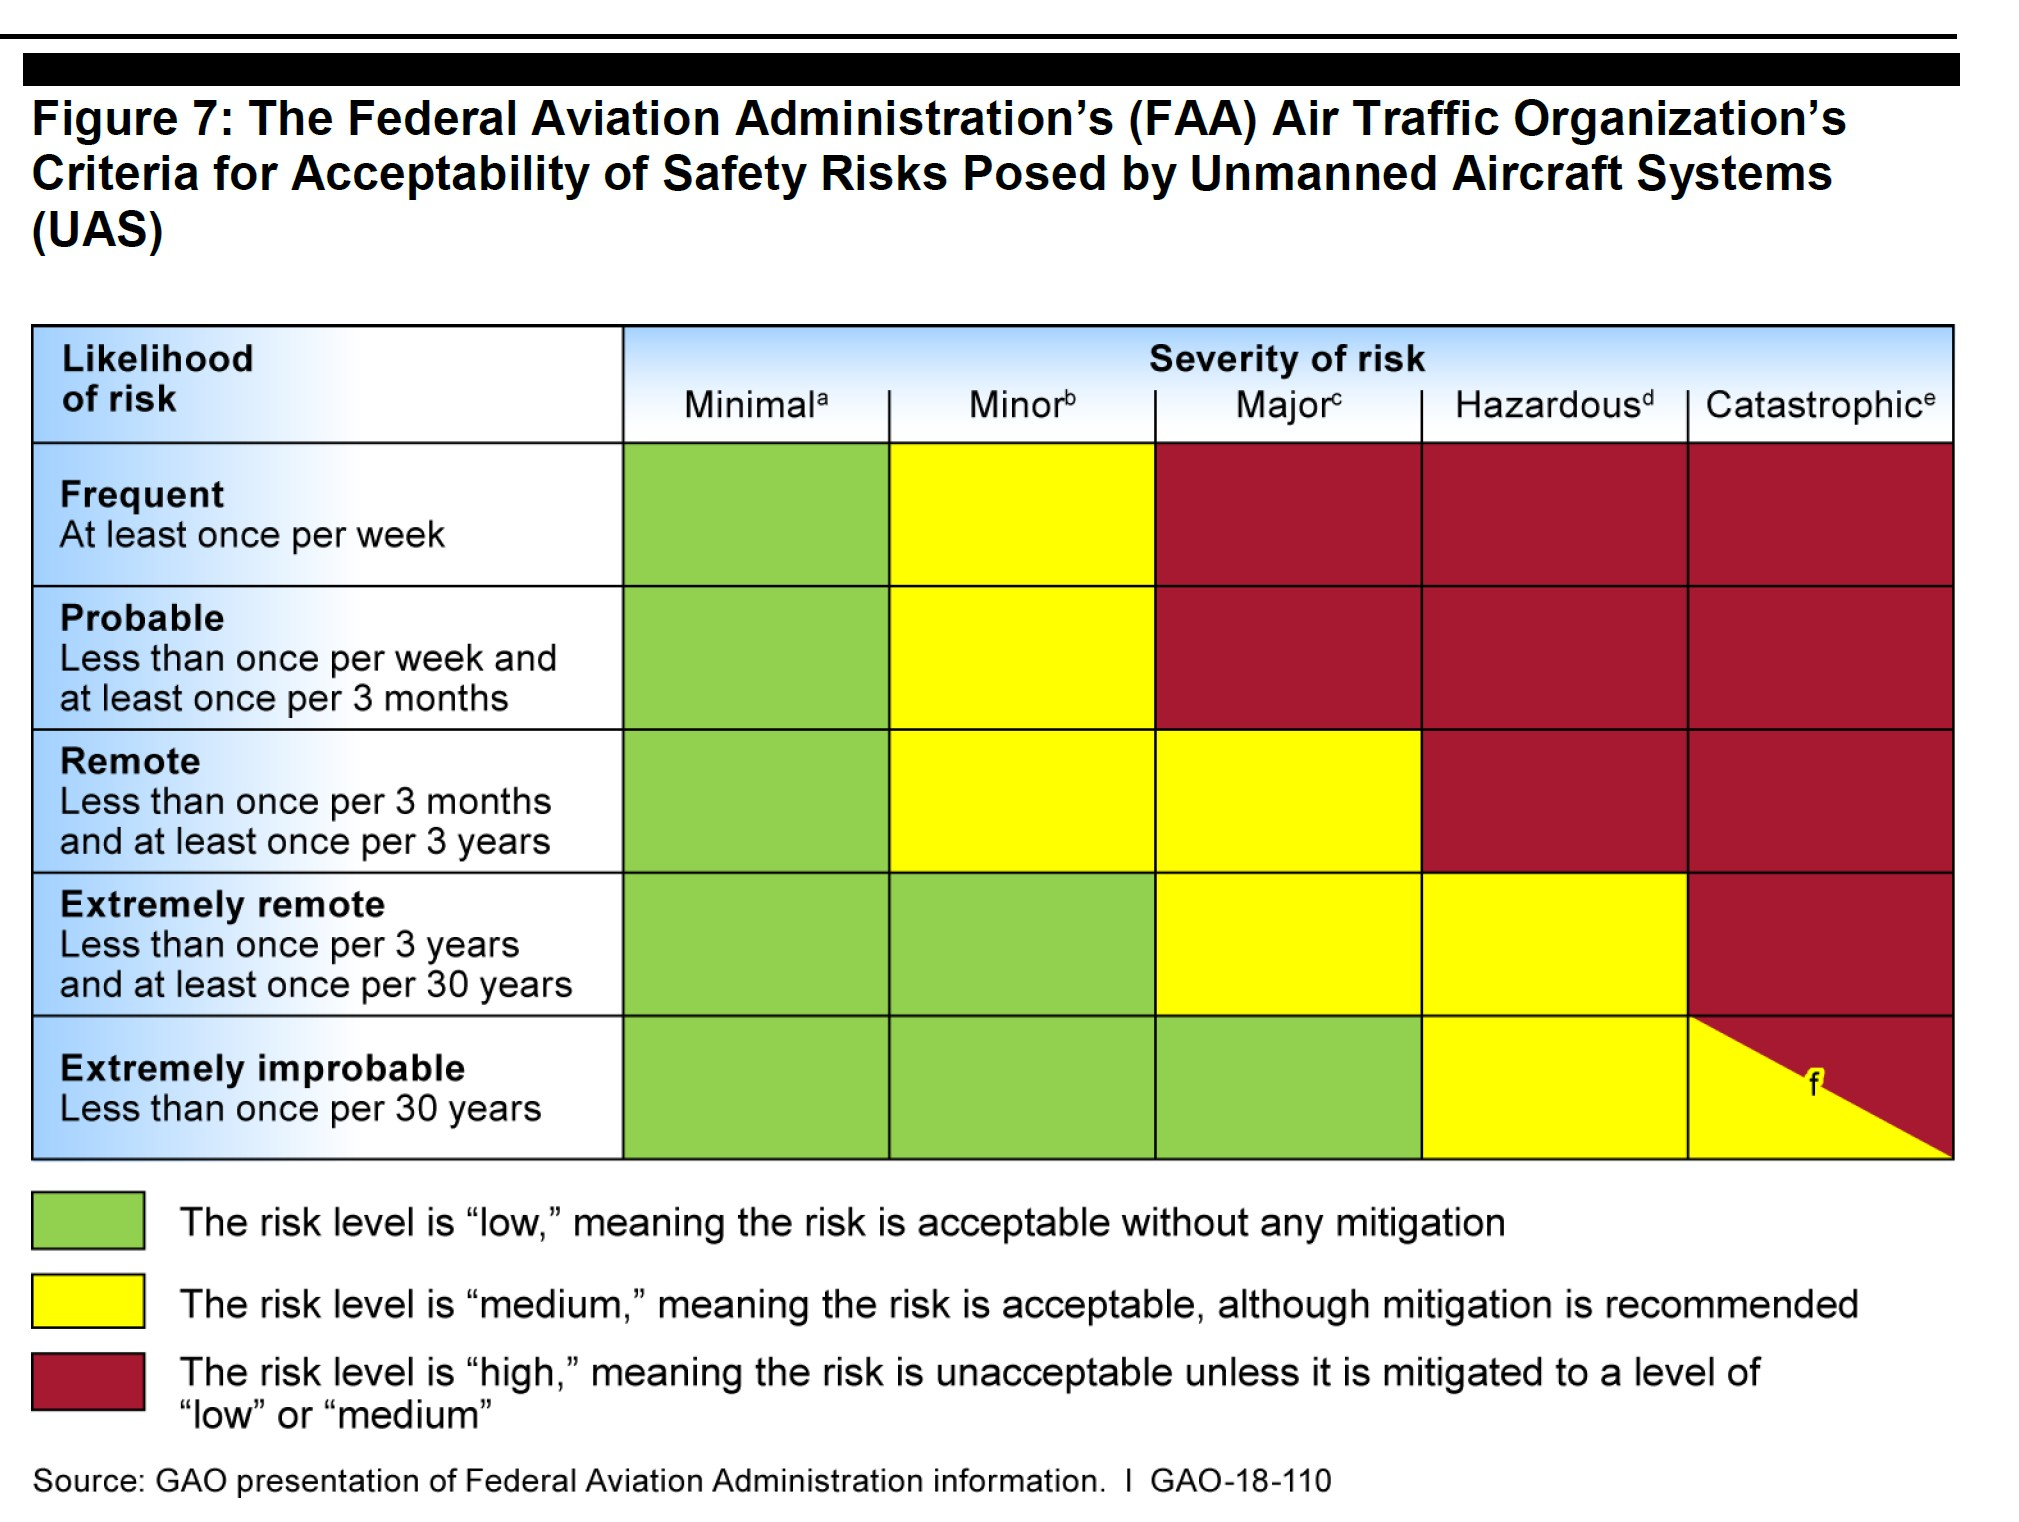
\includegraphics[width=0.8\linewidth]{images/Risk_Matrix} 

}

\caption{Recently Published Risk Matrix from the FAA}\label{fig:risk-matrix}
\end{figure}

\hypertarget{hazard-severity}{%
\section{Hazard Severity}\label{hazard-severity}}

The FAA defines severity as the consequence or impact of a hazard's effect or outcome in terms of degree of loss or harm.

\begin{itemize}
\item
  Minimal severity refers to outcomes in which a UAS causes discomfort to those on the ground.
\item
  Minor severity refers to outcomes in which a UAS causes non-serious injury to three or fewer people on the ground.
\item
  Major severity refers to outcomes in which

  \begin{itemize}
  \tightlist
  \item
    a UAS causes non-serious injury to more than three people on the ground;
  \item
    a UAS crew experiences a reduced ability to cope with adverse operating conditions to the extent that there would be a significant reduction in safety margins; or
  \item
    a UAS causes a manned aircraft to make an evasive maneuver, but the UAS and the manned aircraft remain greater than 500 feet apart.
  \end{itemize}
\item
  Hazardous severity refers to outcomes in which

  \begin{itemize}
  \tightlist
  \item
    the UAS crew is incapacitated;
  \item
    a UAS flies within 500 feet of a manned aircraft; or
  \item
    a UAS causes injury to persons other than the UAS crew.
  \end{itemize}
\item
  Catastrophic severity refers to outcomes in which

  \begin{itemize}
  \tightlist
  \item
    a UAS collides with a manned aircraft or
  \item
    a UAS causes a fatality or fatal injury to one or more persons other than the UAS crew.
  \end{itemize}
\end{itemize}

\hypertarget{likelihood}{%
\section{Likelihood}\label{likelihood}}

The FAA defines likelihood as the estimated probability or frequency in quantitative or qualitative terms of a hazard's effect or outcome.

\begin{itemize}
\tightlist
\item
  Frequent - at least once per week.
\item
  Probable - less than once per week and at least once per 3 months.
\item
  Remote - less than once per 3 months and at least once per 3 years.
\item
  Extremely Remote - less than once per 3 years and at least once per 30 years.
\item
  Extremely Improbable - less than once per 30 years.
\end{itemize}

\hypertarget{analysis}{%
\section{Analysis}\label{analysis}}

The Risk Matrix in Figure \ref{fig:risk-matrix} can be utilized to determine whether or not a particular hazard requires mitigation. It also provides insight to the FAA's safety approach.

Observations:

\begin{itemize}
\tightlist
\item
  The FAA labels a UAS-manned aircraft as a catastrophic incident and that it is only tolerable without mitigation if it occurs less frequently than once per 30 years.\\
\item
  The FAA labels equivalent risk severity for injury a spectator as a UAS flying within 500 ft of a manned aircraft.
\item
  Injuring a member (or three) of the UAS crew is considered a minor severity and any hazard that may cause it to happen more frequently than once per 3 years recommends mitigation.
\end{itemize}

\hypertarget{ch-request}{%
\chapter{Example Flight Request Information}\label{ch-request}}

Thank you for reaching out to us to use UAS on our campus. Before we can approve your usage, we must validate that the activity is legal, will be conducted safely and will not interfere with \protect\hyperlink{UB}{University Business}.

Please provide the following information, if applicable, or your contingency plan:

\begin{itemize}
\item
  \protect\hyperlink{RPC}{Remote Pilot Certificate} with sUAS rating, or other legal authorization
\item
  Aircraft Registrations
\item
  Certificate of Insurance
\item
  Proposed Flight plan, annotated map preferred
\item
  Safety plans (if appropriate)

  \begin{itemize}
  \tightlist
  \item
    Emergency Procedures
  \item
    Crew management
  \item
    Crowd control
  \end{itemize}
\end{itemize}

In general, the proposed operation should not be to fly over campus indiscriminately. The \protect\hyperlink{RPIC}{RPIC} should select specific flight routes or areas with clear visibility to intruding air traffic and intruding pedestrian traffic and designed such that risks can be effectively managed. Chapter \ref{ch-example-terms} provides a list of common terms of approval that may be utilized in order to approve \protect\hyperlink{UASactivity}{UAS activity}.

\hypertarget{ch-example-terms}{%
\chapter{Example Terms of Approval}\label{ch-example-terms}}

The Policy does not mandate specific terms for approval for \protect\hyperlink{UASactivity}{UAS activity}. However, there are many situations where special terms of approval should be required. Below includes a handful of common conditions found in Terms of Approvals from a wide range of \protect\hyperlink{UASactivity}{UAS activity} proposed in the past year.

\textbf{Notification Requirements}

\begin{itemize}
\tightlist
\item
  Must notify \protect\hyperlink{DLA}{Designated Local Authority} at least 24 hours in advance
\item
  Must coordinate with facility manager
\item
  No prior notification required
\item
  Must notify campus PD at least 72 hours in advance
\item
  Must check in with front office prior to flight
\item
  Must call airport manager at least 45 minutes before flight
\end{itemize}

\textbf{Communication Requirements}

\begin{itemize}
\tightlist
\item
  Constant communication not required
\item
  A supporting ground crew member must monitor an aviation radio
\item
  \protect\hyperlink{RPIC}{RPIC} must be reachable via radio during the event
\end{itemize}

\textbf{Operational Limitations}

\begin{itemize}
\tightlist
\item
  Flight altitude restricted to under 200 ft \protect\hyperlink{AGL}{AGL}
\item
  \protect\hyperlink{UA}{Unmanned Aircraft} must remain at least 50 ft away from any non-participants
\item
  \protect\hyperlink{UA}{Unmanned Aircraft} racing path must run parallel to the flight line
\item
  \protect\hyperlink{UA}{Unmanned Aircraft} may not fly over trees or buildings
\item
  \protect\hyperlink{UA}{Unmanned Aircraft} must stay below the tree line
\item
  \protect\hyperlink{UA}{Unmanned Aircraft} may not be flown for more than 7 minutes at a time
\item
  \protect\hyperlink{UA}{Unmanned Aircraft} may not be flown within 150 ft of a residential window
\end{itemize}

\textbf{Safety Enhancements}

\begin{itemize}
\tightlist
\item
  At least 2 \protect\hyperlink{VO}{Visual Observers} are required
\item
  All participants should wear a high visibility safety vest or conspicous professional attire.
\item
  Utilize additiona ground personnel for crowd control to ensure that non-participants do not enter the flight area.
\item
  A UC staff member must be onsite during all \protect\hyperlink{UASactivity}{UAS activity}.
\end{itemize}

\textbf{Currency Requirements}

\begin{itemize}
\tightlist
\item
  The \protect\hyperlink{RPIC}{RPIC} must have logged three launch and landings with a \protect\hyperlink{UA}{Unmanned Aircraft} of the same make/model within the past 90 days.
\item
  The \protect\hyperlink{RPIC}{RPIC} must have logged six night-time \protect\hyperlink{UASactivity}{UAS activity} within the past 90 days.
\item
  The \protect\hyperlink{RPIC}{RPIC} must have logged three launch and landings of a similar \protect\hyperlink{riskscore}{Risk Score} or higher within the past 90 days.
\end{itemize}

\textbf{Post Flight Reporting}

\begin{itemize}
\tightlist
\item
  \protect\hyperlink{RPIC}{RPIC} must submit a post-flight report within 2 days of the \protect\hyperlink{UASactivity}{UAS activity}.
\item
  \protect\hyperlink{RPIC}{RPIC} must submit a set of post-flight reports at the end of every month, no later than 5 business days after the end of the month.
\item
  Course Instructor must submit a proposal of indoor activities and expected usage in lieu of post-flight reporting.
\end{itemize}

\hypertarget{ch-example-denial}{%
\chapter{Example Denial Template}\label{ch-example-denial}}

Thank you for utilizing UC Drones to request a UAS flight. UAS flights are reviewed on a case-by-case basis for compliance with federal, state, and local laws as well as impacts on safety and privacy by the UC Center of Excellence on UAS Safety, Campus Risk Management, and University police. Unfortunately, we cannot allow this flight activity for one or more of the following reasons:

\textbf{LEGAL OR POLICY ISSUES}

\begin{itemize}
\tightlist
\item
  The proposed flight operations are prohibited by campus policies
\item
  The proposed pilot does not have the correct Federal Aviation Administration Pilot Certificate
\item
  The proposed pilot does not have the requisite Federal Aviation Administration Airspace Authorization or Airspace Waiver
\item
  The aircraft is not correctly registered as a non-model aircraft with the FAA while being used for non-recreational purposes
\item
  The proposed flight operation would violate FAA regulations without special authorization from the FAA

  \begin{itemize}
  \tightlist
  \item
    Night operations (14 CFR 107.29)
  \item
    Visual line of sight (14 CFR 107.31)
  \item
    Flight over people (14 CFR 107.39)
  \item
    Other:
  \end{itemize}
\item
  The proposed flight operation would violate FAA regulation. Cite all applicable:
\item
  The proposed flight operation would violate Public Law 112-95, Section 336 -- Special Rule for Model Aircraft. Cite all applicable:
\item
  The proposed pilot does not have sufficient aviation liability coverage.
\item
  Other, please describe:
\end{itemize}

\textbf{SAFETY ISSUES}

\begin{itemize}
\tightlist
\item
  The proponent did not provide evidence of insurance
\item
  The proponent did not provide a sufficient safety case for operating near non-participants
\item
  The proponent did not provide a sufficient safety case for operating near vehicular traffic
\item
  The proposed pilot has not demonstrated sufficient skill for the operation
\item
  The proposed flight altitude is unsuitable for the proposed flight location
\item
  The proposed flight location contains numerous hazards
\item
  Environmental conditions reduce the safety of the operation past acceptable levels
\item
  There are other flights in the area at a similar time
\item
  Other, please describe:
\end{itemize}

\textbf{PRIVACY ISSUES}

\begin{itemize}
\tightlist
\item
  The flight passes close by sensitive areas without proper precautions
\item
  The operation carelessly collects data from bystanders
\item
  The flight is in an area where people have a reasonable sense of privacy
\item
  There is a history of privacy violations from members involved in the operation
\item
  Other, please describe:
\end{itemize}

Rejection of a UAS operation is not limited to the list above, but serves to provide common cases for dismissal. Rejection may be a result of extenuating circumstances, compounding risks, or other factors that are not included on this list. This list may be subject to change in the future, due to changes in FAA law, campus policy, or local and state legislation. As such is important to consider these factors when submitting a flight request and attempt to address all non-listed concerns prior to submission.

\hypertarget{ch-policy-full-text}{%
\chapter{UAS Policy Full Text}\label{ch-policy-full-text}}

\hypertarget{policy-statement}{%
\section{Policy Statement}\label{policy-statement}}

The University recognizes that UAS and Small UAS offer great potential as tools for research and other educational functions as well as providing opportunities for recreational use and business pursuits across a diverse array of users and industries. The University also has an obligation to consider public safety, privacy, civil rights, and civil liberties issues related to the use of UAS.

This Policy establishes a \protect\hyperlink{SDA}{Systemwide Designated UAS Authority} and a \protect\hyperlink{AB}{UAS Advisory Board} to provide oversight of the use of UAS and to develop and implement policies and guidance for the use of UAS. Executive Officers may assign a \protect\hyperlink{DLA}{Designated Local Authority} and authorize the development and implementation of location specific policies and procedures at any \protect\hyperlink{UL}{University Location} within the Executive Officer's jurisdiction. A \protect\hyperlink{DLA}{Designated Local Authority} may be authorized to provide oversight at a \protect\hyperlink{UL}{University Location}.

It is the policy of the University that anyone who seeks to operate a University-owned UAS, a UAS for \protect\hyperlink{UB}{University Business} or on a \protect\hyperlink{UL}{University Location} must comply with the following:

\begin{itemize}
\tightlist
\item
  Have approval from the appropriate aviation agency and operate in compliance with all applicable regulations and rulings.
\item
  Receive approval in advance from the \protect\hyperlink{DLA}{Designated Local Authority} at a specific \protect\hyperlink{UL}{University Location} or \protect\hyperlink{SDA}{Systemwide Designated UAS Authority}.
\item
  Operate in a manner that ensures public safety, right to privacy, civil rights and civil liberties.
\item
  Maintain sufficient liability insurance coverage.
\end{itemize}

A University \protect\hyperlink{LSP}{location specific policy or procedure} may further define an approval process or processes that addresses recurrent, standing, conditional or other forms of approval that constitute written approval. Additional conditions or restrictions may be agreed upon and attached to the approval. A University \protect\hyperlink{LSP}{location specific policy or procedure} may additionally further define \protect\hyperlink{UASactivity}{UAS activity} reporting requirements.

Some exceptions from the provisions in this Policy may be made on a case by case basis after review and approval by the \protect\hyperlink{AB}{UAS Advisory Board}, which shall consider and balance relevant factors such as human health and safety, environmental concerns, privacy, the purpose of the proposed \protect\hyperlink{UASactivity}{UAS activity}, and operator experience. The justification for any such exceptions shall be documented in writing by the \protect\hyperlink{AB}{UAS Advisory Board}.

\hypertarget{complianceresponsibilities}{%
\section{Compliance/Responsibilities}\label{complianceresponsibilities}}

The goal of this Policy is to ensure that all UAS activities are conducted in a manner that ensures the protection of students, faculty, staff, visitors, the public, property, and the environment and complies with all applicable laws and regulations.
The following individuals have the particular responsibilities for implementing the principles and practices of this Policy.

\hypertarget{executive-officer-or-their-designees-are-responsible-for}{%
\subsection{Executive Officer or their designees are responsible for:}\label{executive-officer-or-their-designees-are-responsible-for}}

\begin{itemize}
\tightlist
\item
  Communicating the University's commitment to individual's rights safety, privacy, civil rights, and civil liberties.
\item
  Oversight of the interpretation and effective implementation of this Policy at University Locations within their jurisdiction.
\item
  Adopting procedures to ensure implementation of this UAS Policy.
\item
  Authorizing the development and implementation of University location specific policy or procedures, as applicable.
\item
  Assigning a \protect\hyperlink{DLA}{Designated Local Authority} as a point of contact who is responsible for developing, implementing, and enforcing \protect\hyperlink{UL}{University Location}-specific requirements, as applicable.
\end{itemize}

\hypertarget{the-university-of-california-office-of-the-president-ucop-environment-health-safety-ehs-executive-director-is-responsible-for}{%
\subsection{The University of California Office of the President (UCOP) Environment, Health \& Safety (EH\&S) Executive Director is responsible for:}\label{the-university-of-california-office-of-the-president-ucop-environment-health-safety-ehs-executive-director-is-responsible-for}}

\begin{itemize}
\tightlist
\item
  Providing Policy interpretation and responding to general inquiries regarding UAS Activities.
\item
  Enforcing the provisions of this Policy.
\item
  Assigning a \protect\hyperlink{SDA}{Systemwide Designated UAS Authority}.
\item
  Maintaining records of the results and decisions of the \protect\hyperlink{SDA}{Systemwide Designated UAS Authority}.
\item
  Making UAS records publically available as appropriate.
\item
  Appointing members to the \protect\hyperlink{AB}{UAS Advisory Board}.
\end{itemize}

\hypertarget{the-refsda-is-responsible-for}{%
\subsection{The \protect\hyperlink{SDA}{Systemwide Designated UAS Authority} is responsible for:}\label{the-refsda-is-responsible-for}}

\begin{itemize}
\tightlist
\item
  Providing UAS regulatory interpretation and assistance with compliance.
\item
  Ensuring Policy compliance with applicable laws and regulations.
\item
  Providing assistance with requests for UAS activities consistent with applicable laws and regulations and Policy requirements, unless a \protect\hyperlink{DLA}{Designated Local Authority} has been selected and delegated this task for specific University Locations.
\item
  Providing support in communication with regulatory authorities, and when appropriate, acting on behalf of University faculty and staff as a point of contact to the applicable aviation authority for UAS registration and flight operations.
\item
  Providing a central repository for all applicable regulations and policies, including international, federal, state and local regulations, and UC \protect\hyperlink{LSP}{location specific policy or procedure} and other agency policies, as appropriate.
\item
  Maintaining a record of \protect\hyperlink{UASactivity}{UAS activity} covered under this Policy.
\item
  Implementing effective mechanisms for reporting in order to remain in compliance with applicable laws and policies.
\item
  Providing a forum to communicate and share UAS-related information and best practices.
\item
  Coordinating the development of University UAS policies through task forces/working groups.
\end{itemize}

\hypertarget{the-refab-is-responsible-for}{%
\subsection{The \protect\hyperlink{AB}{UAS Advisory Board} is responsible for:}\label{the-refab-is-responsible-for}}

\begin{itemize}
\tightlist
\item
  Reviewing exceptions from this Policy on a case-by-case basis, subject to the requirements in Section III, above.
\item
  Assisting in the development of systemwide UAS policies.
\item
  Reviewing and commenting on proposed policies and long-term goals.
\item
  Evaluating the effectiveness of systemwide UAS policies and safety metrics.
\item
  Ensuring that systemwide UAS policies remain consistent with applicable privacy best practices.
\end{itemize}

\hypertarget{a-refdla-if-assigned-by-an-executive-officer-or-hisher-designee-is-responsible-for}{%
\subsection{A \protect\hyperlink{DLA}{Designated Local Authority} (if assigned by an Executive Officer or his/her designee) is responsible for:}\label{a-refdla-if-assigned-by-an-executive-officer-or-hisher-designee-is-responsible-for}}

\begin{itemize}
\tightlist
\item
  Developing \protect\hyperlink{LSP}{location specific policy or procedure} that meet or exceed the requirements of this Policy.
\item
  Providing assistance with requests for UAS activity consistent with applicable laws and regulations and University Location-specific policies or procedures.
\item
  Reviewing and approving applications for operation of UAS within the \protect\hyperlink{DLA}{Designated Local Authority}'s jurisdiction.
\item
  Notifying the applicant if the flight authorization request is approved, denied, or if the flight authorization request will require further information or appropriate aviation agency authorization.
\item
  Maintaining a record of approval requests and decisions, which shall be submitted to the \protect\hyperlink{SDA}{Systemwide Designated UAS Authority} upon request.
\item
  Maintaining a record of all UAS flights at University Locations within the \protect\hyperlink{DLA}{Designated Local Authority}'s jurisdiction, which record shall be submitted to the \protect\hyperlink{SDA}{Systemwide Designated UAS Authority} upon request.
\end{itemize}

\hypertarget{operators-of-uas-are-responsible-for}{%
\subsection{Operators of UAS are responsible for:}\label{operators-of-uas-are-responsible-for}}

\begin{itemize}
\tightlist
\item
  Requesting and obtaining all proper approvals prior to operating a UAS at any \protect\hyperlink{UL}{University Location} or for any \protect\hyperlink{UB}{University Business}.
\item
  Following the requirements of this Policy and all applicable laws and regulations.
\item
  Maintaining a safe UAS operating environment.
\item
  Following applicable University UAS privacy best practices.
\item
  Reporting \protect\hyperlink{UASactivity}{UAS activity} to the \protect\hyperlink{DLA}{Designated Local Authority} or \protect\hyperlink{SDA}{Systemwide Designated UAS Authority}.
\item
  Immediately reporting any accident that results in injury or property damage to the \protect\hyperlink{DLA}{Designated Local Authority} or \protect\hyperlink{SDA}{Systemwide Designated UAS Authority}.
\end{itemize}

\hypertarget{required-procedures}{%
\section{Required Procedures}\label{required-procedures}}

This Policy sets minimum systemwide requirements for operating UAS. The requirements below must be followed at all University Locations. Individual campuses, medical centers, Agriculture and Natural Resources locations, and Lawrence Berkeley National Laboratory, through their respective \protect\hyperlink{DLA}{Designated Local Authorities}, may also develop policies and procedures as long as they meet or exceed the requirements of this Policy.
The operation of UAS by emergency first responders may be exempt from this Policy based on determination of emergency needs. During such operations, the emergency responders will follow their internal department protocols.

\hypertarget{general-procedures}{%
\subsection{General Procedures}\label{general-procedures}}

\begin{itemize}
\tightlist
\item
  All persons seeking to operate a University-Owned UAS, a UAS for \protect\hyperlink{UB}{University Business}, or at \protect\hyperlink{UL}{University Location} must first submit a completed \protect\hyperlink{FR}{UAS Request Form} to the \protect\hyperlink{DLA}{Designated Local Authority} or \protect\hyperlink{SDA}{Systemwide Designated UAS Authority} in advance of any \protect\hyperlink{UASactivity}{UAS activity}.
\item
  The \protect\hyperlink{DLA}{Designated Local Authority} or \protect\hyperlink{SDA}{Systemwide Designated UAS Authority} will review and process the request and notify the applicant if the request is approved, denied, or will require further information no later than two weeks after submission of an application.
\item
  The request must be reviewed for

  \begin{itemize}
  \tightlist
  \item
    Compliance with applicable regulations and policies
  \item
    Impacts to public safety
  \item
    Impacts to privacy
  \item
    Impacts to civil rights and civil liberties
  \item
    Compliance with insurance requirements
  \end{itemize}
\item
  Once approved, the operator must follow the requirements of this Policy, any conditions required by the approval, and all applicable laws and regulations.
\item
  A copy of the approval must be in the possession of the operator at all times during the activity and, upon request, must be presented to any University official or representative with jurisdiction over the activity.
\item
  The operator must follow University privacy best practices at all times, including, but not limited to:
\item
  UAS may not be used to monitor or record activities where there is a reasonable expectation of privacy.
\item
  UAS must not be used for unapproved recordings of any campus events or performances, or for any unlawful purpose.
\item
  The operator must provide a post-flight report of \protect\hyperlink{UASactivity}{UAS activity} to the \protect\hyperlink{DLA}{Designated Local Authority} or \protect\hyperlink{SDA}{Systemwide Designated UAS Authority} as soon as possible.

  \begin{itemize}
  \tightlist
  \item
    Any accident that results in injury or property damage must be reported immediately.
  \end{itemize}
\end{itemize}

\hypertarget{registration-of-uas}{%
\subsection{Registration of UAS}\label{registration-of-uas}}

\begin{itemize}
\tightlist
\item
  All UC-owned UAS must be registered in accordance with all applicable laws, regulations, and requirements.
\item
  Registration documents for UC-owned UAS must be submitted to the \protect\hyperlink{DLA}{Designated Local Authority} or \protect\hyperlink{SDA}{Systemwide Designated UAS Authority} and must reflect the following ownership data:
\end{itemize}

\begin{quote}
The Regents of the University of California\\
(University Location Address)
\end{quote}

\begin{itemize}
\tightlist
\item
  Registration documents for all UAS used for \protect\hyperlink{UB}{University Business} must be submitted to the \protect\hyperlink{DLA}{Designated Local Authority} or \protect\hyperlink{SDA}{Systemwide Designated UAS Authority}.
\end{itemize}

\hypertarget{liability-insurance}{%
\subsection{Liability Insurance}\label{liability-insurance}}

\begin{itemize}
\tightlist
\item
  All \protect\hyperlink{UASactivity}{UAS activity} covered under this Policy must have aviation liability coverage.
\item
  Any 3rd Party or Non-\protect\hyperlink{UB}{University Business} \protect\hyperlink{UASactivity}{UAS activity} must additionally include a written agreement that indemnifies and holds the University harmless from any claims or harm to individuals, damage to University property, and any other claims, liabilities, and potential penalties.
\item
  Recreational users, at the discretion of the \protect\hyperlink{DLA}{Designated Local Authority}, may be exempt from the liability insurance requirement if the \protect\hyperlink{DLA}{Designated Local Authority} determines that the proposed recreational use poses no risk to the health and safety of persons, property, or the environment and that the cost of liability insurance would pose an undue hardship to the recreational user.
\end{itemize}

\hypertarget{export-control}{%
\subsection{Export Control}\label{export-control}}

\begin{itemize}
\tightlist
\item
  All \protect\hyperlink{UASactivity}{UAS activity} for \protect\hyperlink{UB}{University Business} in foreign nations or by foreign nationals must follow export control regulations and the UC Export Control Policy.
\item
  All \protect\hyperlink{UASactivity}{UAS activity} involving the export of a UAS internationally or use of an export-controlled UAS must be reviewed by the appropriate export control officer.
\end{itemize}

\hypertarget{ch-UAS-regs-details}{%
\chapter{UAS Regulations in Detail}\label{ch-UAS-regs-details}}

\hypertarget{s-part107}{%
\section{14 CFR 107 - SMALL UNMANNED AIRCRAFT SYSTEMS}\label{s-part107}}

The introduction of 14 CFR 107 enabled a wide range of small UAS usage under a set of defined limitations. A Compliance List for 14 CFR 107 is provided below.

\hypertarget{operator-requirements}{%
\subsection{Operator Requirements}\label{operator-requirements}}

\begin{itemize}
\item
  A person operating an sUAS must either

  \begin{itemize}
  \tightlist
  \item
    hold a \protect\hyperlink{RPC}{Remote Pilot Certificate} with an sUAS rating
  \item
    or be under the direct supervision of a person who does hold a \protect\hyperlink{RPC}{Remote Pilot Certificate} (\protect\hyperlink{RPIC}{RPIC}).
  \end{itemize}
\item
  A person may not operate an sUAS if he or she knows or has reason to know of any physical or mental condition that would interfere with the safe operation of an sUAS.
\item
  Foreign nationals are allowed to operate under Part 107 if they satisfy the requirements of 14 CFR 375. Typical allowances:

  \begin{itemize}
  \tightlist
  \item
    Non-commercial operations
  \item
    Recreational activity
  \item
    Specific research activities
  \item
    Foreign nationals from Canada or Mexico (Order 97-7-3, FAA)
  \end{itemize}
\end{itemize}

\hypertarget{aircraft-requirements-ss-aircraft}{%
\subsection{Aircraft Requirements \{ss-aircraft\}}\label{aircraft-requirements-ss-aircraft}}

\begin{itemize}
\tightlist
\item
  Unmanned aircraft must weigh less than 55 lbs. (25 kg).
\item
  Unmanned aircraft must be registered with either a `N' number or an `FA' number (Under 14 CFR 47 or 48).
\item
  Unmanned aircraft must be inspected prior to flight by the remote pilot in command.
\end{itemize}

\hypertarget{airspace-requirements}{%
\subsection{Airspace Requirements}\label{airspace-requirements}}

\begin{itemize}
\tightlist
\item
  Operations in Class G airspace are allowed without Air Traffic Control permission.
\item
  Operations in Class B, C, D and E airspace are allowed with an \protect\hyperlink{AA}{Airspace Authorization} or \protect\hyperlink{AW}{Airspace Waiver}. Operating limitations are specified within a \protect\hyperlink{COA}{COA} (Form 7711) provided by the \protect\hyperlink{FAA}{FAA}.
\end{itemize}

\hypertarget{operating-limitations}{%
\subsection{Operating Limitations}\label{operating-limitations}}

\begin{itemize}
\tightlist
\item
  \protect\hyperlink{VLOS}{VLOS} only.
\end{itemize}

\begin{quote}
Note: The unmanned aircraft must always remain within \protect\hyperlink{VLOS}{VLOS} of the remote pilot in command and the person manipulating the flight controls of the sUAS, even if they are not directly looking at it at every instance.
\end{quote}

\begin{itemize}
\tightlist
\item
  At all times the sUAS must remain close enough to the \protect\hyperlink{RPIC}{RPIC} and the person manipulating the flight controls of the sUAS for those people to be capable of seeing the aircraft with vision unaided by any device other than corrective lenses.
\end{itemize}

\begin{quote}
Note: First-Person View cameras do not satisfy \protect\hyperlink{VLOS}{VLOS} or visual contact regulations, but may be used.
\end{quote}

\begin{itemize}
\tightlist
\item
  An sUAS may not operate over any persons not directly participating in the operation, not under a covered structure, and not inside a covered stationary vehicle.
\end{itemize}

\begin{quote}
Note: Prior notice and/or consent is not sufficient.
\end{quote}

\begin{itemize}
\tightlist
\item
  Daylight-only operations, or civil twilight (30 minutes before official sunrise to 30 minutes after official sunset, local time) with appropriate anti-collision lighting.
\item
  Maximum groundspeed of 100 mph (87 knots).
\item
  Maximum altitude of 400 feet AGL or, if higher than 400 feet AGL, remain within 400 feet of a structure.
\item
  Minimum weather visibility of 3 miles from control station.
\item
  No person may act as a \protect\hyperlink{RPIC}{RPIC} or \protect\hyperlink{VO}{Visual Observer} for more than one unmanned aircraft operation at one time.
\item
  No operations from a moving aircraft.
\item
  No operations from a moving vehicle unless the operation is over a sparsely populated area.
\item
  No careless or reckless operations.
\item
  No carriage of hazardous materials.
\item
  External load operations are allowed if the object being carried by the unmanned aircraft is securely attached and does not adversely affect the flight characteristics or controllability of the aircraft.
\item
  Transportation of property for compensation or hire allowed provided that-

  \begin{itemize}
  \tightlist
  \item
    The aircraft, including its attached systems, payload and cargo weigh less than 55 pounds total;
  \item
    The flight is conducted within visual line of sight and not from a moving vehicle or aircraft; and
  \item
    The flight occurs wholly within the bounds of a State and does not involve transport between (1) Hawaii and another place in Hawaii through airspace outside Hawaii; (2) the District of Columbia and another place in the District of Columbia; or (3) a territory or possession of the United States and another place in the same territory or possession.
  \end{itemize}
\end{itemize}

\hypertarget{s-recreation}{%
\section{Exception for Limited Recreational Operations of Unmanned Aircraft}\label{s-recreation}}

A person may operate a small UAS without specific certification or operating authority from the FAA if the operation adheres to all of the following limitations:

\begin{itemize}
\tightlist
\item
  The aircraft is flown strictly for recreational purposes.
\item
  The aircraft is operated in accordance with or within the programming of a community-based organization's set of safety guidelines that are developed in coordination with the Federal Aviation Administration.
\item
  The aircraft is flown within the visual line of sight of the person operating the aircraft or a visual observer co-located and in direct communication with the operator.
\item
  The aircraft is operated in a manner that does not interfere with and gives way to any manned aircraft.
\item
  In Class B, Class C, or Class D airspace or within the lateral boundaries of the surface area of Class E airspace designated for an airport, the operator obtains prior authorization from the Administrator or designee before operating and complies with all airspace restrictions and prohibitions.
\item
  In Class G airspace, the aircraft is flown from the surface to not more than 400 feet above ground level and complies with all airspace restrictions and prohibitions.
\item
  The operator has passed an aeronautical knowledge and safety test described in subsection (g) and maintains proof of test passage to be made available to the Administrator or law enforcement upon request.
\item
  The aircraft is registered and marked in accordance with chapter 441 of this title and proof of registration is made available to the Administrator or a designee of the Administrator or law enforcement upon request.
\end{itemize}

\hypertarget{definition-of-hobby-or-recreational-use}{%
\subsection{Definition of Hobby or Recreational Use}\label{definition-of-hobby-or-recreational-use}}

Hobby or recreational use is defined as

\begin{itemize}
\tightlist
\item
  Operated for fun or outside of one's regular occupation
\item
  Operated in furtherance of one's education at an accredited educational institution
\end{itemize}

Activities that do not qualify for Model Aircraft Regulations

\begin{itemize}
\tightlist
\item
  Commercial activity with compensation
\item
  Commercial activity without compensation
\item
  Activity in furtherance of a business
\end{itemize}

\hypertarget{use-of-unmanned-aircraft-systems-at-institutions-of-higher-education}{%
\subsection{Use of Unmanned Aircraft Systems at Institutions of Higher Education}\label{use-of-unmanned-aircraft-systems-at-institutions-of-higher-education}}

For the purposes of the exception for limited recreational operations of unmanned aircraft, a `recreational purpose' shall include an unmanned aircraft system operated by an institution of higher education for educational or research purposes.

Educational or Research purposes includes

\begin{itemize}
\tightlist
\item
  Instruction of students at the institution;
\item
  Academic or research related uses of unmanned aircraft systems that have been approved by the institution, including Federal Research;
\item
  Activities undertaken by the institution as part of research projects, including research projects sponsored by the Federal Government; and
\item
  Other academic activities approved by the institution
\end{itemize}

\hypertarget{definition-of-community-based-organization-set-of-safety-guidelines}{%
\subsection{Definition of Community-based organization set of safety guidelines}\label{definition-of-community-based-organization-set-of-safety-guidelines}}

A Community-Based Organization means a membership-based association entity that

\begin{itemize}
\tightlist
\item
  is described in section 501(c)(3) of the Internal Revenue Code of 1986;
\item
  is exempt from tax under section 501(a) of the Internal Revenue Code of 1986;
\item
  the mission of which is demonstrably the furtherance of model aviation;
\item
  provides a comprehensive set of safety guidelines for all aspects of model aviation addressing the assembly and operation of model aircraft and that emphasize safe aeromodelling operations within the national airspace system and the protection and safety of individuals and property on the ground, and may provide a comprehensive set of safety rules and programming for the operation of unmanned aircraft that have the advanced flight capabilities enabling active, sustained, and controlled navigation of the aircraft beyond visual line of sight of the operator;
\item
  provides programming and support for any local charter organizations, affiliates, or clubs; and
\item
  provides assistance and support in the development and operation of locally designated model aircraft flying sites.
\end{itemize}

The FAA has interpreted this statement as community-based organizations would include groups such as the \protect\hyperlink{AMA}{Academy of Model Aeronautics} and others that meet the statuary definition.

\hypertarget{s-safety-code}{%
\section{Representative Safety Code}\label{s-safety-code}}

Reprinted from \protect\hyperlink{AMA}{Academy of Model Aeronautics} Safety Code: \url{https://www.modelaircraft.org/files/105.pdf}

\begin{content-box}{green}

\textbf{Academy of Model Aeronautics}\\
National Model Aircraft Safety Code\\
Effective January 1, 2018

A model aircraft is a non-human-carrying device capable of sustained flight within visual line of sight of the pilot or spotter(s). It may not exceed limitations of this code and is intended exclusively for sport, recreation, education and/or competition. All model flights must be conducted in accordance with this safety code and related AMA guidelines, any additional rules specific to the flying site, as well as all applicable laws and regulations.
As an AMA member I agree:

\begin{itemize}
\tightlist
\item
  I will not fly a model aircraft in a careless or reckless manner.
\item
  I will not interfere with and will yield the right of way to all human-carrying aircraft using AMA's See and Avoid Guidance and a spotter when appropriate.
\item
  I will not operate any model aircraft while I am under the influence of alcohol or any drug that could adversely affect my ability to safely control the model.
\item
  I will avoid flying directly over unprotected people, moving vehicles, and occupied structures.
\item
  I will fly Free Flight (FF) and Control Line (CL) models in compliance with AMA's safety programming.
\item
  I will maintain visual contact of an RC model aircraft without enhancement other than corrective lenses prescribed to me. When using an advanced flight system, such as an autopilot, or flying First-Person View (FPV), I will comply with AMA's Advanced Flight System programming.
\item
  I will only fly models weighing more than 55 pounds, including fuel, if certified through AMA's Large Model Airplane Program.
\item
  I will only fly a turbine-powered model aircraft in compliance with AMA's Gas Turbine Program.
\item
  I will not fly a powered model outdoors closer than 25 feet to any individual, except for myself or my helper(s) located at the flightline, unless I am taking off and landing, or as otherwise provided in AMA's Competition Regulation.
\item
  I will use an established safety line to separate all model aircraft operations from spectators and bystanders.
\end{itemize}

\end{content-box}

Additional information can be found in the \protect\hyperlink{AMA}{Academy of Model Aeronautics} Safety Handbook: \url{http://www.modelaircraft.org/files/100.pdf}

\hypertarget{ch-resources}{%
\chapter{Additional Resources}\label{ch-resources}}

\hypertarget{faa-resources}{%
\section{FAA Resources}\label{faa-resources}}

\begin{figure}

{\centering 
\includegraphics[width=0.6\linewidth]{images/FAA_logo} 

}

\caption{Federal Aviation Administration}\label{fig:faa-logo}
\end{figure}

FAA Website: \url{http://www.faa.gov}

Recreational Flyers \& Modeler Community-Based Organizations: \url{https://www.faa.gov/uas/recreational_fliers/}

Certificated Remote Pilots including Commercial Operators: \url{https://www.faa.gov/uas/commercial_operators/}

Educational Users: \url{https://www.faa.gov/uas/educational_users/}

Policy Document Library: \url{https://www.faa.gov/uas/resources/policy_library/}

\hypertarget{uc-center-of-excellence-on-uas-safety}{%
\section{UC Center of Excellence on UAS Safety}\label{uc-center-of-excellence-on-uas-safety}}

\begin{center}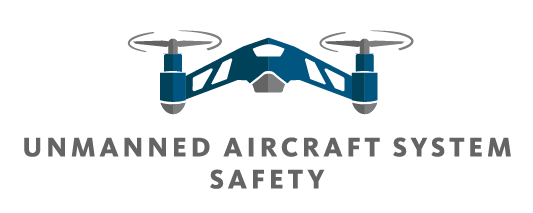
\includegraphics[width=0.5\linewidth]{images/COE_logo} \end{center}

Website: \url{https://www.ucop.edu/safety-and-loss-prevention/environmental/program-resources/unmanned-aircraft-systems-safety.html}

UC Drones Web Application: \url{http://ehs.ucop.edu/drones}

UC Drones Document Library: \url{https://ucdrones.github.io/}

\hypertarget{regulations}{%
\section{Regulations}\label{regulations}}

United States Code

Public Law

\begin{itemize}
\tightlist
\item
  Public Law 112-95, Title III, Subtitle B- Unmanned Aircraft Systems - Section 331-336: \url{https://www.faa.gov/uas/programs_partnerships/uas_arctic/media/Sec_331_336_UAS.pdf}
\item
  Public Law 114-90, Title II, Subtitle B - UAS Safety: \url{https://www.faa.gov/uas/resources/uas_regulations_policy/media/Pages-from-PLAW-114publ190.pdf}
\end{itemize}

Code of Federal Regulations

\begin{itemize}
\tightlist
\item
  14 CFR 1 - DEFINITIONS, CIVIL AIRCRAFT
\item
  14 CFR 47 - AIRCRAFT REGISTRATION
\item
  14 CFR 48 - REGISTRATION AND MARKING REQUIREMENTS FOR SMALL UNMANNED AIRCRAFT
\item
  14 CFR 91 - GENERAL OPERATING AND FLIGHT RULES
\item
  14 CFR 101 - MOORED BALLOONS, KITES, AMATEUR ROCKETS, UNMANNED FREE BALLOONS, AND CERTAIN MODEL AIRCRAFT
\item
  14 CFR 107 - SMALL UNMANNED AIRCRAFT SYSTEMS
\end{itemize}

\hypertarget{glossary}{%
\chapter{Glossary}\label{glossary}}

\hypertarget{AGL}{%
\subsubsection*{Above Ground Level}\label{AGL}}
\addcontentsline{toc}{subsubsection}{Above Ground Level}

The term \protect\hyperlink{AGL}{Above Ground Level} refers to the height measured with respect to the underlying ground surface.





\hypertarget{AMA}{%
\subsubsection*{Academy of Model Aeronautics}\label{AMA}}
\addcontentsline{toc}{subsubsection}{Academy of Model Aeronautics}

The Academy of Model Aeronautics (AMA) is an model aviation association.



\hypertarget{aircraft}{%
\subsubsection*{Aircraft}\label{aircraft}}
\addcontentsline{toc}{subsubsection}{Aircraft}

An aircraft is defined as a device that is used or intended to be used for flight in the air.



\hypertarget{AA}{%
\subsubsection*{Airspace Authorization}\label{AA}}
\addcontentsline{toc}{subsubsection}{Airspace Authorization}

The term \protect\hyperlink{AA}{Airspace Authorization} means a short term or temporary authorization granted by the \protect\hyperlink{FAA}{FAA} to a specific organization or person to operate within controlled airspace. An `Airspace Authorization' may be granted with a \protect\hyperlink{COA}{COA} or through (ref:LAANC).





\hypertarget{AW}{%
\subsubsection*{Airspace Waiver}\label{AW}}
\addcontentsline{toc}{subsubsection}{Airspace Waiver}

The term \protect\hyperlink{AW}{Airspace Waiver} means a long term authorization granted by the \protect\hyperlink{FAA}{FAA} to a specific organization or person to operate within controlled airspace. An `Airspace Waiver' is granted with a \protect\hyperlink{COA}{COA}.





\hypertarget{BVLOS}{%
\subsubsection*{Beyond Visual Line of Sight}\label{BVLOS}}
\addcontentsline{toc}{subsubsection}{Beyond Visual Line of Sight}

The term \protect\hyperlink{BVLOS}{Beyond Visual Line of Sight} means that a person is operating a UAS beyond the definition of \protect\hyperlink{VLOS}{Visual Line of Sight}.





\hypertarget{currency}{%
\subsubsection*{Currency}\label{currency}}
\addcontentsline{toc}{subsubsection}{Currency}

The term \protect\hyperlink{currency}{currency} means to demonstrate that one's skills and flight experience are `current' or up-to-date. Currency may be defined with respect to a category, class or type of aircraft and is defined with respect to a specific time-interval.



\hypertarget{COA}{%
\subsubsection*{Certificate of Waiver or Authorization}\label{COA}}
\addcontentsline{toc}{subsubsection}{Certificate of Waiver or Authorization}

The term \protect\hyperlink{COA}{Certificate of Waiver or Authorization (COA)} means an authorization issued by the Air Traffic Organization, a division of the Federal Aviation Administration (FAA), for UAS operations. A COA is filed on FAA Form 7711.





\hypertarget{CBO}{%
\subsubsection*{Community-Based Organization}\label{CBO}}
\addcontentsline{toc}{subsubsection}{Community-Based Organization}

The term \protect\hyperlink{CBO}{Community-Based Organization} means a membership-based association entity that (1) is described in Section 501(c)(3) of the IRS Code of 1986; (2) is exempt from tax under section 501(a) of the IRS Code of 1986; (3) the mission of which is demonstrably the furtherance of model aviation; (4) provides a comprehensive set of safety guidelines for all aspects of model aviation addressing the assembly and operation of model aircraft and that emphasize safe aeromodelling operations within the national airspace system and the protection and safety of individuals and property on the ground, and may provide a comprehensive set of safety rules and programming for the operation of unmanned aircraft that have the advanced flight capabilities enabling active, sustained, and controlled navigation of the aircraft beyond visual line of sight of the operator; (5) provides programming and support for any local charter organizations, affiliates, or clubs; and (6) provides assistance and support in the development and operation of locally designated model aircraft flying sites. At this point, the FAA has not released an advisory circular that identifies the criteria and process required for recognition of community-based organizations.





\hypertarget{DLA}{%
\subsubsection*{Designated Local Authority}\label{DLA}}
\addcontentsline{toc}{subsubsection}{Designated Local Authority}

The \protect\hyperlink{DLA}{Designated Local Authority} is a single-point of contact or committee appointed by an \protect\hyperlink{EO}{Executive Officer} at an individual \protect\hyperlink{UL}{University Location} to oversee the development, implementation, and enforcement of any University Location-specific UAS related policies and procedures.





\hypertarget{drone}{%
\subsubsection*{Drone}\label{drone}}
\addcontentsline{toc}{subsubsection}{Drone}

The term \protect\hyperlink{drone}{drone} is a colloquial or common synonymous with \protect\hyperlink{UAS}{Unmanned Aircraft System}.



\hypertarget{EO}{%
\subsubsection*{Executive Officer}\label{EO}}
\addcontentsline{toc}{subsubsection}{Executive Officer}

The \protect\hyperlink{EO}{Executive Officer} means any of the University of California's Chancellors, Medical Center Chief Executive Officers, Director of Lawrence Berkeley National Laboratory, and Vice President for Agriculture and Natural Resources.



\hypertarget{FAA}{%
\subsubsection*{Federal Aviation Administration}\label{FAA}}
\addcontentsline{toc}{subsubsection}{Federal Aviation Administration}

The \protect\hyperlink{FAA}{Federal Aviation Administration} is a division of the United States Department of Transportation that inspects and rates civilian aircraft and pilots, enforces the rules of air safety, and installs and maintains air-navigation and traffic-control facilities.





\hypertarget{LiPo}{%
\subsubsection*{Lithium Polymer}\label{LiPo}}
\addcontentsline{toc}{subsubsection}{Lithium Polymer}

The term \protect\hyperlink{LiPo}{LiPo} refers to the regular use Lithium Polymer batteries within UAS. These are now common in most electronics due to their light weight and high energy capacity. However, unlike other batteries, they need special care for charging, discharging and storage.



\hypertarget{LSP}{%
\subsubsection*{Location Specific Policy or Procedure}\label{LSP}}
\addcontentsline{toc}{subsubsection}{Location Specific Policy or Procedure}

The term \protect\hyperlink{LSP}{location specific policy or procedure} means a policy or procedure, or a set of policies or procedures, established at a \protect\hyperlink{UL}{University Location}. The policy or procedure must include a review as described in Chapter \ref{ch-review}, but may be flexible to address a diverse set of \protect\hyperlink{UASactivity}{UAS activity}.





\hypertarget{NAS}{%
\subsubsection*{National Airspace System}\label{NAS}}
\addcontentsline{toc}{subsubsection}{National Airspace System}

The term \protect\hyperlink{NAS}{National Airspace System} (NAS) means the common network of U.S. airspace, including all navigable airspace from the ground up, excluding regions under military jurisdiction. The NAS additionally does not include inside of buildings or enclosed structures.





\hypertarget{NTSB}{%
\subsubsection*{National Traffic Safety Board}\label{NTSB}}
\addcontentsline{toc}{subsubsection}{National Traffic Safety Board}

The \protect\hyperlink{NTSB}{National Traffic Safety Board} is an independent U.S. government investigative agency responsible for civil transportation accident investigation, including aviation and UAS accidents.



\hypertarget{PA}{%
\subsubsection*{Public Aircraft}\label{PA}}
\addcontentsline{toc}{subsubsection}{Public Aircraft}

The term \protect\hyperlink{PA}{Public Aircraft} means an aircraft owned and operated by the government of a State, the District of Columbia, or a territory or possession of the United States or a political subdivision of one of these governments, except when the aircraft is operated for commercial purposes.



\hypertarget{PAO}{%
\subsubsection*{Public Agency Operation}\label{PAO}}
\addcontentsline{toc}{subsubsection}{Public Agency Operation}

The term \protect\hyperlink{PAO}{PAO} means an operation conducted by a \protect\hyperlink{PA}{Public Aircraft} that is used for a governmental function as defined by Title 49 USC 40125(a)(2). Specific \protect\hyperlink{UASactivity}{UAS activity} within the UC may be eligible for PAO status. Whether an operation qualifies as a PAO is determined on a flight-by-flight basis.





\hypertarget{RPC}{%
\subsubsection*{Remote Pilot Certificate}\label{RPC}}
\addcontentsline{toc}{subsubsection}{Remote Pilot Certificate}

The term \protect\hyperlink{RPC}{Remote Pilot Certificate} means a certificate issued by the \protect\hyperlink{FAA}{FAA} that certifies that the owner of the certificate has sufficient aerospace knowledge to operate an \protect\hyperlink{UA}{Unmanned Aircraft} within the \protect\hyperlink{NAS}{National Airspace System}. It may also be referred to as a `Drone License.'



\hypertarget{RPIC}{%
\subsubsection*{Remote Pilot in Command}\label{RPIC}}
\addcontentsline{toc}{subsubsection}{Remote Pilot in Command}

The term \protect\hyperlink{RPIC}{RPIC} means the person who as the final authority and responsibility for the operation and safety of an \protect\hyperlink{UAS}{UAS} operation. This may or may not be the person operating the \protect\hyperlink{UA}{Unmanned Aircraft}. A person may manipulate the controls of a unmanned aircraft under the direct and immediate supervision of an \protect\hyperlink{RPIC}{RPIC}.







\hypertarget{riskscore}{%
\subsubsection*{Risk Score}\label{riskscore}}
\addcontentsline{toc}{subsubsection}{Risk Score}

For the purposes of this document, the term \protect\hyperlink{riskscore}{Risk Score} refers to a customized Risk Score between 1-5 that communicates an approximately level of risk; ranging from minor to severe (potential to cause injury or significant property damage). See Section () for a description of the \protect\hyperlink{riskscore}{Risk Score} and scoring matrix.



\hypertarget{sUAS}{%
\subsubsection*{Small Unmanned Aircraft System}\label{sUAS}}
\addcontentsline{toc}{subsubsection}{Small Unmanned Aircraft System}

The term \protect\hyperlink{sUAS}{Small Unmanned Aircraft System} means an \protect\hyperlink{UA}{Unmanned Aircraft} weighing less than 55 lbs. and associated elements that are required to operate safely and efficiently in the national airspace system.





\hypertarget{SDA}{%
\subsubsection*{Systemwide Designated UAS Authority}\label{SDA}}
\addcontentsline{toc}{subsubsection}{Systemwide Designated UAS Authority}

The term \protect\hyperlink{SDA}{Systemwide Designated UAS Authority} refers to the authority appointed by the University of California Office of the President (UCOP) Environment, Health \& Safety (EH\&S) Executive Director. The responsibilities of the \protect\hyperlink{SDA}{Systemwide Designated UAS Authority} include providing interpretation of \protect\hyperlink{UAS}{UAS} regulations, developing \protect\hyperlink{UAS}{UAS} policies and procedures, maintaining records of all \protect\hyperlink{UASactivity}{UAS activity} and ensuring regulatory compliance.



\hypertarget{TFR}{%
\subsubsection*{Temporary Flight Restriction}\label{TFR}}
\addcontentsline{toc}{subsubsection}{Temporary Flight Restriction}







\hypertarget{postflight}{%
\subsubsection*{UAS Post-Flight Report}\label{postflight}}
\addcontentsline{toc}{subsubsection}{UAS Post-Flight Report}

The term \protect\hyperlink{postflight}{UAS Post-Flight Report} refers to a documented submission of a record of \protect\hyperlink{UASactivity}{UAS activity}. More information on \protect\hyperlink{postflight}{Post-Flight Reports} can be found in Chapter \ref{ch-reporting}.







\hypertarget{FR}{%
\subsubsection*{UAS Request Form}\label{FR}}
\addcontentsline{toc}{subsubsection}{UAS Request Form}

The term \protect\hyperlink{FR}{UAS Request Form} or \protect\hyperlink{FR}{Flight Request} refers to a documented request to operate a UAS pursuant to this Policy. The Policy does not mandate a specific form or system as long as the minimum review criteria is met. See Chapter \ref{ch-review} for further details.





\hypertarget{UCDrones}{%
\subsubsection*{UC Drones}\label{UCDrones}}
\addcontentsline{toc}{subsubsection}{UC Drones}

UC Drones is an online application developed by UC Risk and Safety Solutions that enables users to submit UAS requests and document UAS activity. The \protect\hyperlink{SDA}{Systemwide Designated UAS Authority} and the \protect\hyperlink{DLA}{Designated Local Authorities} may utilize UC Drones to review UAS activity.



\hypertarget{ANR}{%
\subsubsection*{UC Agriculture and Natural Resources}\label{ANR}}
\addcontentsline{toc}{subsubsection}{UC Agriculture and Natural Resources}

The \protect\hyperlink{ANR}{UC Division of Agriculture and Natural Resources} (UC ANR) is a division of the University of California system that connects the power of UC research in agriculture, natural resources, nutrition, and youth development with local communities. UC ANR statewide programs includes 4-H, Cooperative Extensions, Master Gardener Program, and includes a system of Research and Extension Centers across California.



\hypertarget{NRS}{%
\subsubsection*{UC Natural Reserve System}\label{NRS}}
\addcontentsline{toc}{subsubsection}{UC Natural Reserve System}

The \protect\hyperlink{NRS}{UC Natural Reserve System} (UC NRS) is a system of protected ecosystems owned or managed by the University of California that is used for research, education, and public service. The reserves include examples of most of California's major habitat types, from grasslands and deserts to coastal wetlands and conifer forests. With more than 40 sites encompassing some 756,000 acres and growing, the UC NRS is the largest university-administered reserve system in the world.



\hypertarget{UB}{%
\subsubsection*{University Business}\label{UB}}
\addcontentsline{toc}{subsubsection}{University Business}

The term \protect\hyperlink{UB}{University Business} means the official activities of a University that contribute to any one of the University's major functions of teaching, research, patient care, or public service, or to any other non-recreational University purpose.



\hypertarget{UL}{%
\subsubsection*{University Location}\label{UL}}
\addcontentsline{toc}{subsubsection}{University Location}

Any property or building that is owned or leased by the University where University business or activities take place.



\hypertarget{UA}{%
\subsubsection*{Unmanned Aircraft}\label{UA}}
\addcontentsline{toc}{subsubsection}{Unmanned Aircraft}

The term \protect\hyperlink{UA}{Unmanned Aircraft} means an aircraft that is operated without the possibility of direct human intervention from within or on the aircraft. This definition includes aircraft of all sizes.





\hypertarget{UAS}{%
\subsubsection*{Unmanned Aircraft System}\label{UAS}}
\addcontentsline{toc}{subsubsection}{Unmanned Aircraft System}

The term \protect\hyperlink{UAS}{Unmanned Aircraft System} means an \protect\hyperlink{UA}{Unmanned Aircraft} and associated elements (including communication links and the components that control the unmanned aircraft) that are required for the pilot in command to operate safely and efficiently in the national airspace system. For the purposes of this Policy, this includes unmanned aircraft of all sizes and includes unmanned aircraft operated indoors, in military airspace or in foreign airspace systems.







\hypertarget{UASactivity}{%
\subsubsection*{UAS Activity}\label{UASactivity}}
\addcontentsline{toc}{subsubsection}{UAS Activity}

The term \protect\hyperlink{UASactivity}{UAS activity} refers to the act of flying for a defined purposed. It may be used to represent a single flight, a set of flights within a single day, a set of flights across multiple days, and may encompass multiple locations.



\hypertarget{AB}{%
\subsubsection*{UAS Advisory Board}\label{AB}}
\addcontentsline{toc}{subsubsection}{UAS Advisory Board}

The \protect\hyperlink{AB}{UAS Advisory Board} is created by the Policy for the purposes of reviewing and developing future \protect\hyperlink{UAS}{UAS} policies.



\hypertarget{VLOS}{%
\subsubsection*{Visual Line of Sight}\label{VLOS}}
\addcontentsline{toc}{subsubsection}{Visual Line of Sight}

The term \protect\hyperlink{VLOS}{Visual Line of Sight} means that a person is able to 1) know the \protect\hyperlink{UA}{Unmanned Aircraft}'s location, 2) determine the \protect\hyperlink{UA}{Unmanned Aircraft}'s attitude, altitude and direction of flight, 3) observe the airspace for other air traffic or hazards, and 4) determine that the \protect\hyperlink{UA}{Unmanned Aircraft} does not endanger the life or property of another.





\hypertarget{VO}{%
\subsubsection*{Visual Observer}\label{VO}}
\addcontentsline{toc}{subsubsection}{Visual Observer}

The term \protect\hyperlink{VO}{Visual Observer} means a person who is designated by the RPIC to assist the RPIC and the person manipulating the flight controls of the UAS to see and avoid other air traffic or objects aloft or on the ground.





\hypertarget{rdparty}{%
\subsubsection*{\texorpdfstring{3\textsuperscript{rd} Party}{3rd Party}}\label{rdparty}}
\addcontentsline{toc}{subsubsection}{3\textsuperscript{rd} Party}

For the purposes of this document, a \protect\hyperlink{rdparty}{3\textsuperscript{rd} Party} is defined as any person who is conducting \protect\hyperlink{UB}{University Business} but is not affiliated with the UC or any person not conducting \protect\hyperlink{UB}{University Business}.



  \bibliography{book.bib,packages.bib}

\end{document}
